\documentclass[12pt]{extarticle}
\usepackage[paperwidth=18in,paperheight=8.5in]{geometry}
\usepackage{amsmath}
\usepackage{hyperref}
\usepackage{multirow}
\usepackage{pdfpages}
\usepackage[utf8]{inputenc}
\title{Kaon mixing: chiral and continuum extrapolations}
\author{R Mukherjee}
\date{\today}
\begin{document}
\maketitle
\tableofcontents
\clearpage
\begin{figure}
\centering
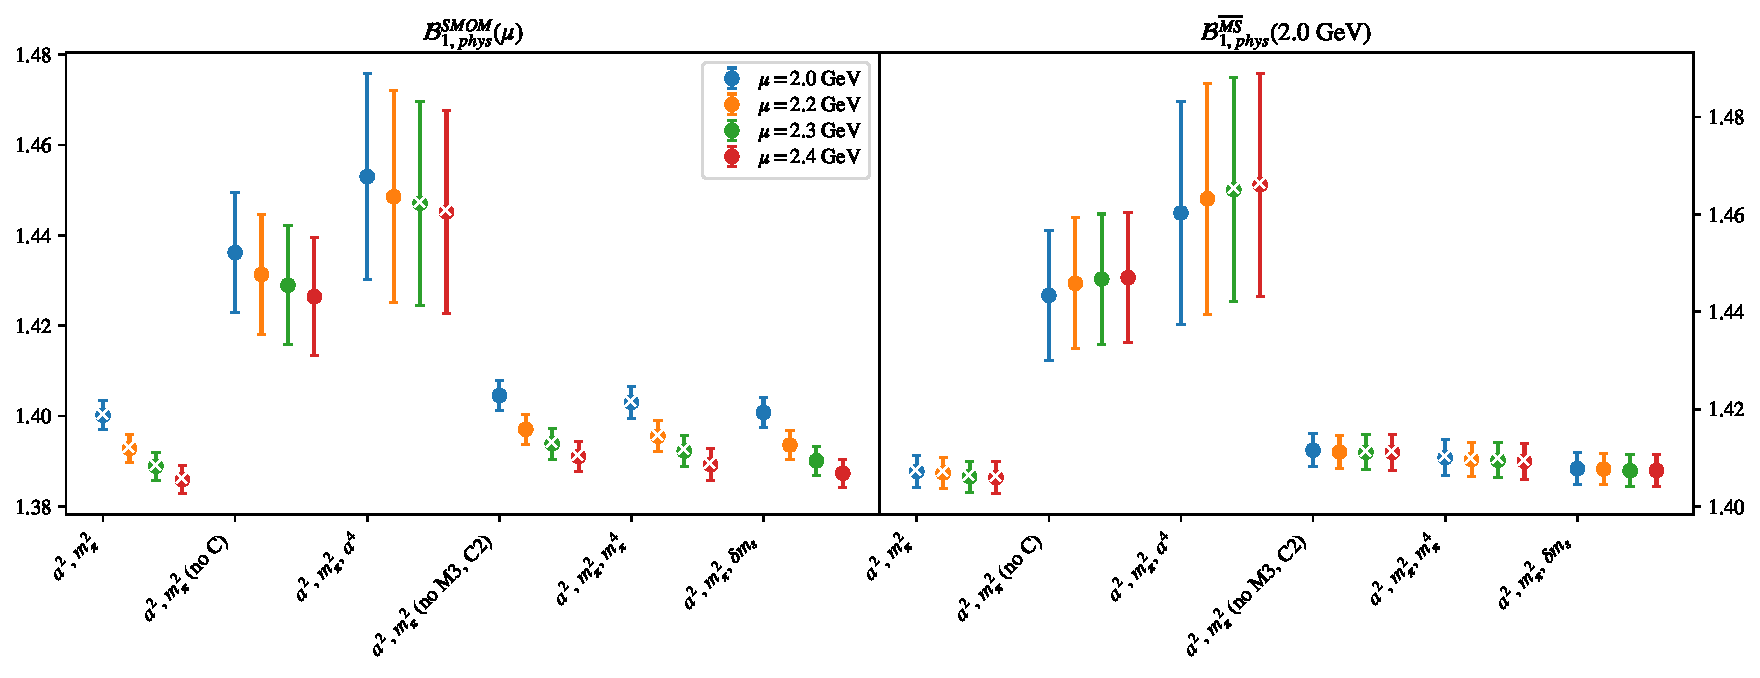
\includegraphics[page=1, width=1.1\textwidth]{VVpAA/NPR/fit_summary_bag.pdf}
\caption{$\mathcal{B}_{1}$\\(left) $\mathcal{B}_{phys}$ in RI/SMOM scheme from fit variations (fits with $p$-value $<0.05$ marked with ``$\times$"). \\(right) $\mathcal{B}_{phys}$ in $\overline{MS}$ computed using $\mathcal{B}^{\overline{MS}} = R^{\overline{MS}\leftarrow SMOM}(2.0)\sigma_{npt}(2.0,\mu) \mathcal{B}^{SMOM}(\mu)$.}
\end{figure}
\clearpage
\begin{figure}
\centering
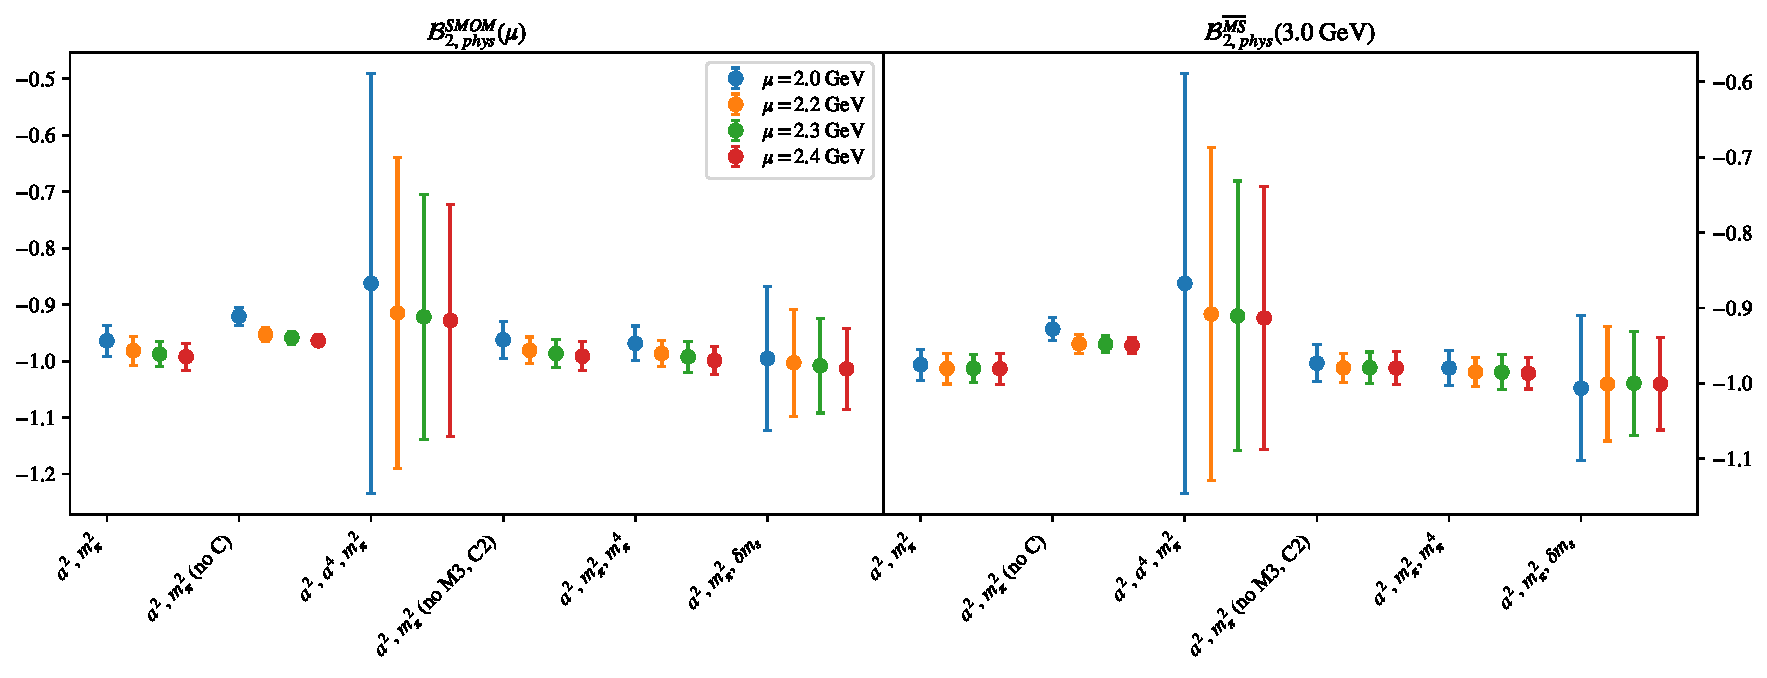
\includegraphics[page=1, width=1.1\textwidth]{VVmAA/NPR/fit_summary_bag.pdf}
\caption{$\mathcal{B}_{2}$\\(left) $\mathcal{B}_{phys}$ in RI/SMOM scheme from fit variations (fits with $p$-value $<0.05$ marked with ``$\times$"). \\(right) $\mathcal{B}_{phys}$ in $\overline{MS}$ computed using $\mathcal{B}^{\overline{MS}} = R^{\overline{MS}\leftarrow SMOM}(3.0)\sigma_{npt}(3.0,\mu) \mathcal{B}^{SMOM}(\mu)$.}
\end{figure}
\clearpage
\begin{figure}
\centering
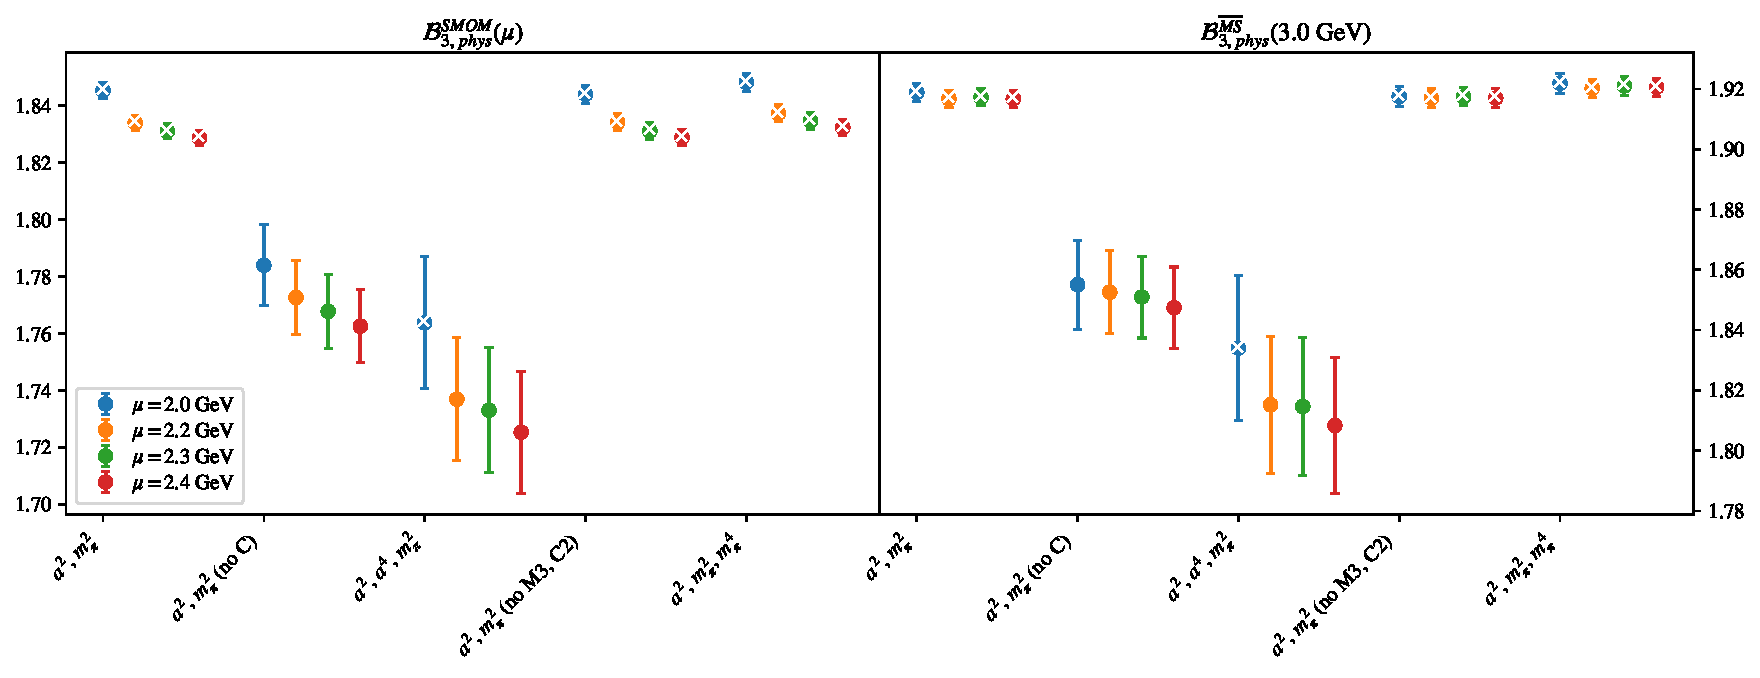
\includegraphics[page=1, width=1.1\textwidth]{SSmPP/NPR/fit_summary_bag.pdf}
\caption{$\mathcal{B}_{3}$\\(left) $\mathcal{B}_{phys}$ in RI/SMOM scheme from fit variations (fits with $p$-value $<0.05$ marked with ``$\times$"). \\(right) $\mathcal{B}_{phys}$ in $\overline{MS}$ computed using $\mathcal{B}^{\overline{MS}} = R^{\overline{MS}\leftarrow SMOM}(3.0)\sigma_{npt}(3.0,\mu) \mathcal{B}^{SMOM}(\mu)$.}
\end{figure}
\clearpage
\begin{figure}
\centering
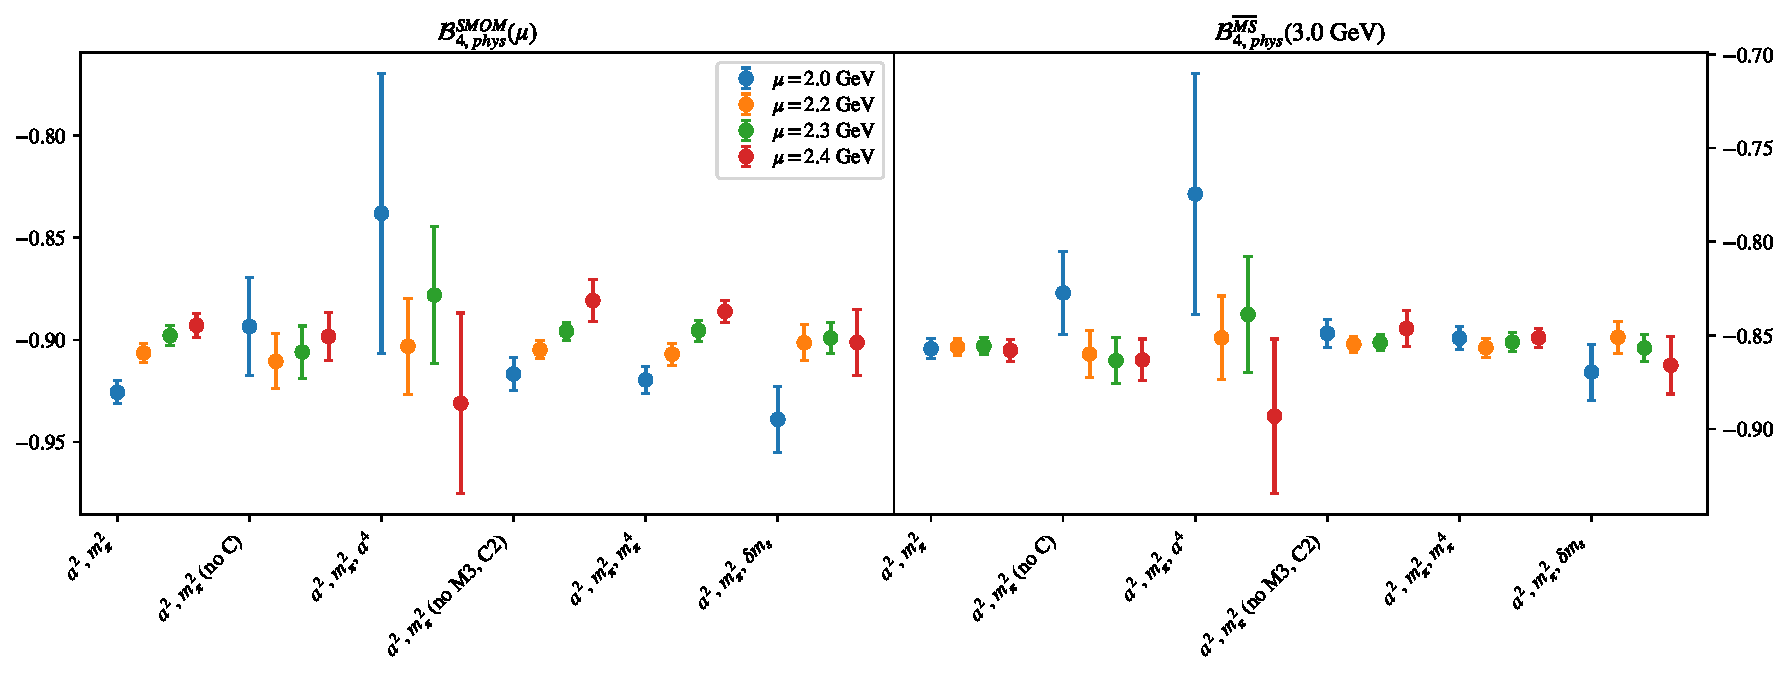
\includegraphics[page=1, width=1.1\textwidth]{SSpPP/NPR/fit_summary_bag.pdf}
\caption{$\mathcal{B}_{4}$\\(left) $\mathcal{B}_{phys}$ in RI/SMOM scheme from fit variations (fits with $p$-value $<0.05$ marked with ``$\times$"). \\(right) $\mathcal{B}_{phys}$ in $\overline{MS}$ computed using $\mathcal{B}^{\overline{MS}} = R^{\overline{MS}\leftarrow SMOM}(3.0)\sigma_{npt}(3.0,\mu) \mathcal{B}^{SMOM}(\mu)$.}
\end{figure}
\clearpage
\begin{figure}
\centering
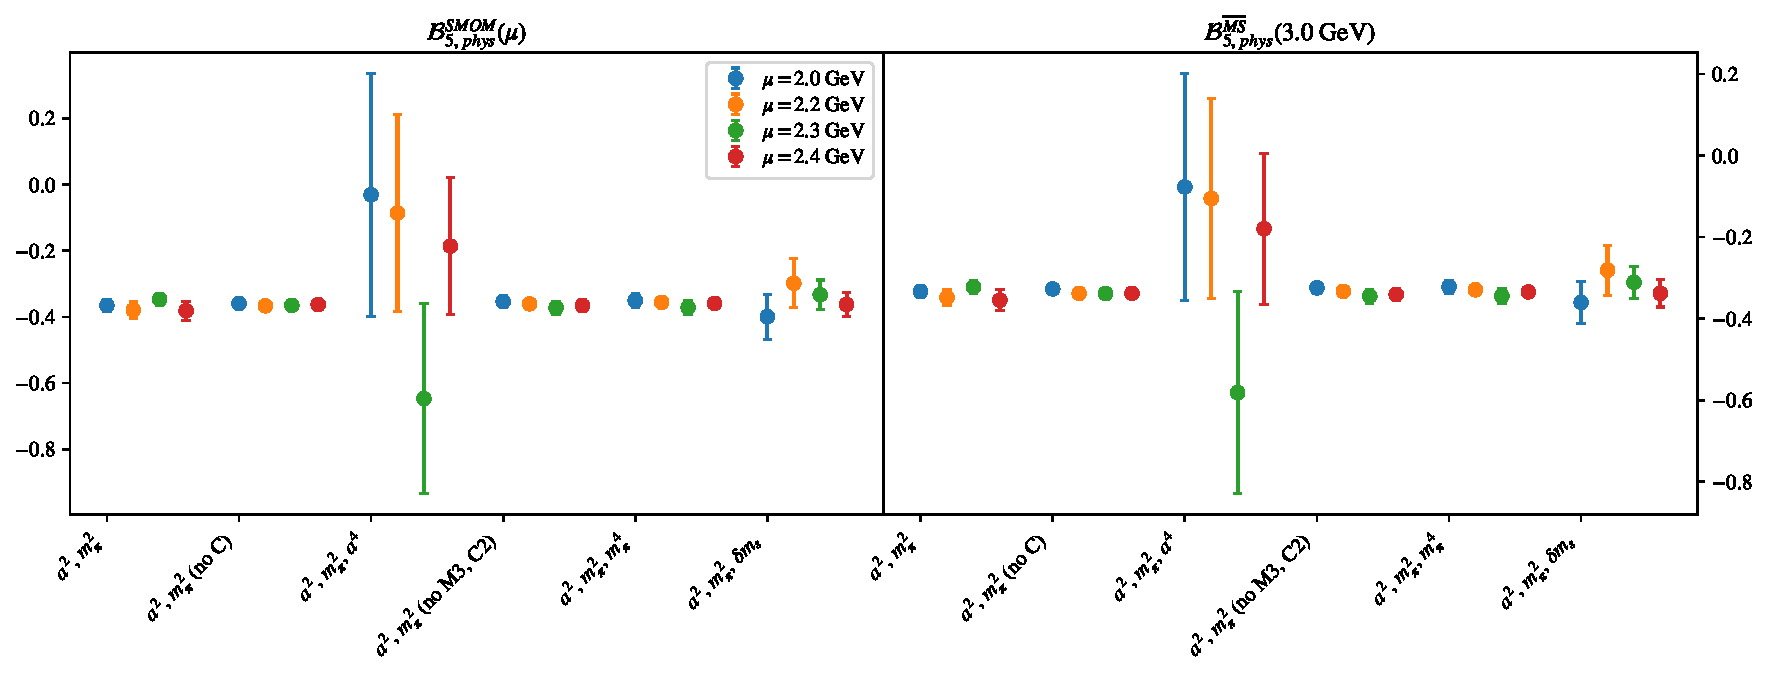
\includegraphics[page=1, width=1.1\textwidth]{TT/NPR/fit_summary_bag.pdf}
\caption{$\mathcal{B}_{5}$\\(left) $\mathcal{B}_{phys}$ in RI/SMOM scheme from fit variations (fits with $p$-value $<0.05$ marked with ``$\times$"). \\(right) $\mathcal{B}_{phys}$ in $\overline{MS}$ computed using $\mathcal{B}^{\overline{MS}} = R^{\overline{MS}\leftarrow SMOM}(3.0)\sigma_{npt}(3.0,\mu) \mathcal{B}^{SMOM}(\mu)$.}
\end{figure}
\clearpage
\section{$\mathcal{B}_1$}
\begin{table}[h!]
\begin{center}
\begin{tabular}{|c|c|c|c|c|c|c|}
\hline
$\mu$ (GeV) & $a^2$, $m_\pi^2$& $a^2$, $m_\pi^2$ (no C)& $a^2$, $m_\pi^2$, $a^4$& $a^2$, $m_\pi^2$ (no M3, C2)& $a^2$, $m_\pi^2$, $m_\pi^4$& $a^2$, $m_\pi^2$, $\delta m_s$\\
\hline
2.0& \hyperlink{VVpAA/NPR/a2m2_20.pdf.1}{\textbf{1.393(11)}: 0.988 (0.423)} & \hyperlink{VVpAA/NPR/a2m2noC_20.pdf.1}{\textbf{1.414(13)}: 0.974 (0.378)} & \hyperlink{VVpAA/NPR/a2a4m2_20.pdf.1}{\textbf{1.445(31)}: 0.872 (0.48)} & \hyperlink{VVpAA/NPR/a2m2mcut_20.pdf.1}{\textbf{1.4034(79)}: 0.254 (0.859)} & \hyperlink{VVpAA/NPR/a2m2m4_20.pdf.1}{\textbf{1.417(12)}: 0.617 (0.65)} & \hyperlink{VVpAA/NPR/a2m2delm_20.pdf.1}{\textbf{1.3979(89)}: 0.821 (0.511)}\\
2.2& \hyperlink{VVpAA/NPR/a2m2_22.pdf.1}{\textbf{1.3962(63)}: 1.179 (0.317)} & \hyperlink{VVpAA/NPR/a2m2noC_22.pdf.1}{\textbf{1.409(13)}: 1.022 (0.36)} & \hyperlink{VVpAA/NPR/a2a4m2_22.pdf.1}{\textbf{1.431(25)}: 1.084 (0.362)} & \hyperlink{VVpAA/NPR/a2m2mcut_22.pdf.1}{\textbf{1.3993(57)}: 0.52 (0.668)} & \hyperlink{VVpAA/NPR/a2m2m4_22.pdf.1}{\textbf{1.3937(87)}: 0.948 (0.435)} & \hyperlink{VVpAA/NPR/a2m2delm_22.pdf.1}{\textbf{1.3960(89)}: 0.948 (0.435)}\\
2.3& \hyperlink{VVpAA/NPR/a2m2_23.pdf.1}{\textbf{1.3916(62)}: 1.313 (0.255)} & \hyperlink{VVpAA/NPR/a2m2noC_23.pdf.1}{\textbf{1.408(13)}: 1.047 (0.351)} & \hyperlink{VVpAA/NPR/a2a4m2_23.pdf.1}{\textbf{1.424(25)}: 1.097 (0.356)} & \hyperlink{VVpAA/NPR/a2m2mcut_23.pdf.1}{\textbf{1.388(10)}: 0.678 (0.566)} & \hyperlink{VVpAA/NPR/a2m2m4_23.pdf.1}{\textbf{1.3968(63)}: 1.121 (0.344)} & \hyperlink{VVpAA/NPR/a2m2delm_23.pdf.1}{\textbf{1.3876(75)}: 0.91 (0.457)}\\
2.4& \hyperlink{VVpAA/NPR/a2m2_24.pdf.1}{\textbf{1.3953(80)}: 1.245 (0.285)} & \hyperlink{VVpAA/NPR/a2m2noC_24.pdf.1}{\textbf{1.406(13)}: 1.073 (0.342)} & \hyperlink{VVpAA/NPR/a2a4m2_24.pdf.1}{\textbf{1.420(26)}: 1.011 (0.4)} & \hyperlink{VVpAA/NPR/a2m2mcut_24.pdf.1}{\textbf{1.3990(75)}: 0.689 (0.559)} & \hyperlink{VVpAA/NPR/a2m2m4_24.pdf.1}{\textbf{1.3987(80)}: 1.133 (0.339)} & \hyperlink{VVpAA/NPR/a2m2delm_24.pdf.1}{\textbf{1.3776(97)}: 1.004 (0.404)}\\
\hline
\end{tabular}
\caption{Physical point value from chiral and continuum extrapolation at renormalisation scale $\mu$. Entries are \textbf{value(error)}: $\chi^2/\text{DOF}$ ($p$-value).}
\end{center}
\end{table}
\begin{table}[h!]
\begin{center}
\begin{tabular}{|c c|c|c|c|c|c|c|}
\hline
$\mu$ (GeV) &  & $a^2$, $m_\pi^2$& $a^2$, $m_\pi^2$ (no C)& $a^2$, $m_\pi^2$, $a^4$& $a^2$, $m_\pi^2$ (no M3, C2)& $a^2$, $m_\pi^2$, $m_\pi^4$& $a^2$, $m_\pi^2$, $\delta m_s$\\
\hline
\multirow{3}{0.5in}{2.0} & $\alpha$ & 0.140(45)& 0.057(58)& -0.2(23)& 0.115(36)& 0.057(45)& 0.123(33)\\
 & $\beta$ & 0.00248(25)& 0.00243(32)& 0.00249(25)& 0.00208(40)& 0.0& 0.00260(28)\\
 & $\gamma$ &  &  & 0.74(56)&  & 0.00021(10)& -0.002(28)\\
\hline
\multirow{3}{0.5in}{2.2} & $\alpha$ & 0.106(24)& 0.049(57)& -0.1(16)& 0.102(24)& 0.124(36)& 0.100(34)\\
 & $\beta$ & 0.00248(24)& 0.00242(32)& 0.00249(23)& 0.00206(39)& 0.001& 0.00259(23)\\
 & $\gamma$ &  &  & 0.50(35)&  & 0.000154(95)& -0.002(29)\\
\hline
\multirow{3}{0.5in}{2.3} & $\alpha$ & 0.111(24)& 0.039(56)& -0.1(16)& 0.131(43)& 0.101(24)& 0.125(28)\\
 & $\beta$ & 0.00247(24)& 0.00241(32)& 0.00251(25)& 0.00202(38)& 0.001& 0.00263(25)\\
 & $\gamma$ &  &  & 0.53(34)&  & 0.000175(91)& -0.003(28)\\
\hline
\multirow{3}{0.5in}{2.4} & $\alpha$ & 0.082(34)& 0.039(56)& -0.09& 0.080(26)& 0.076(30)& 0.140(31)\\
 & $\beta$ & 0.00244(23)& 0.00241(32)& 0.00248(22)& 0.00204(39)& 0.00062(99)& 0.00275(28)\\
 & $\gamma$ &  &  & 0.37(39)&  & 0.000170(89)& -0.007(40)\\
\hline
\end{tabular}
\caption{Fit values of coefficients in $Q = Q_{phys} + \mathbf{\alpha} a^2 + \mathbf{\beta}\left(\frac{m_\pi^2}{f_\pi^2}-\frac{m_{\pi,PDG}^2}{f_\pi^2}\right) + \gamma(\ldots)$}
\end{center}
\end{table}
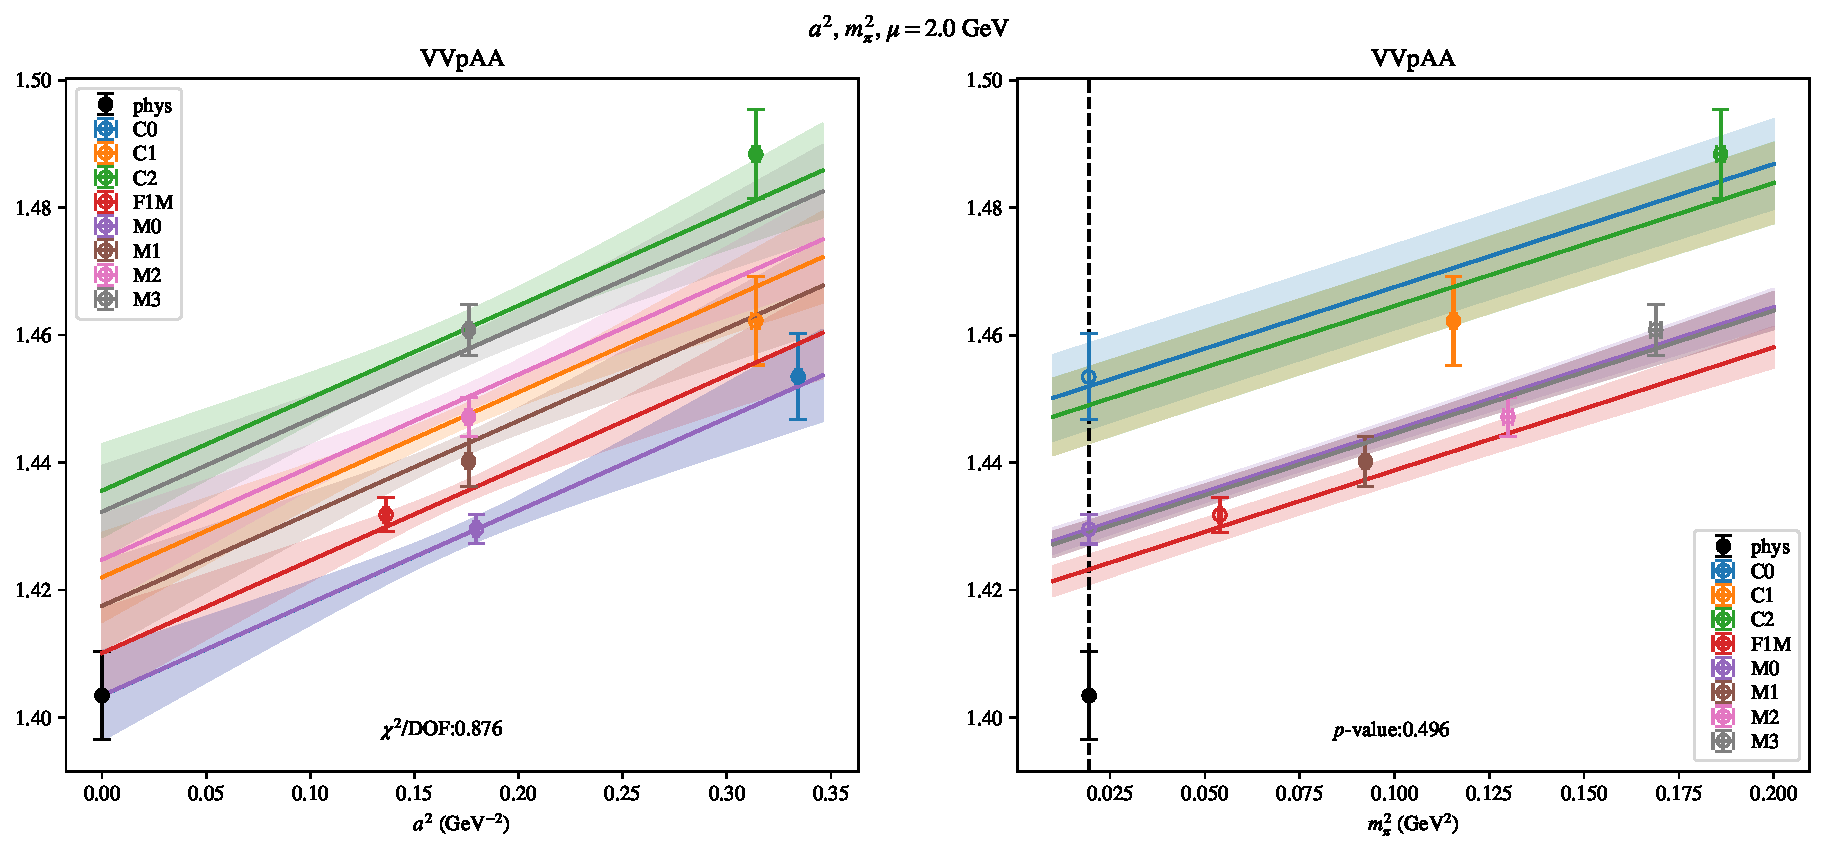
\includepdf[link, pages=-]{VVpAA/NPR/a2m2_20.pdf}
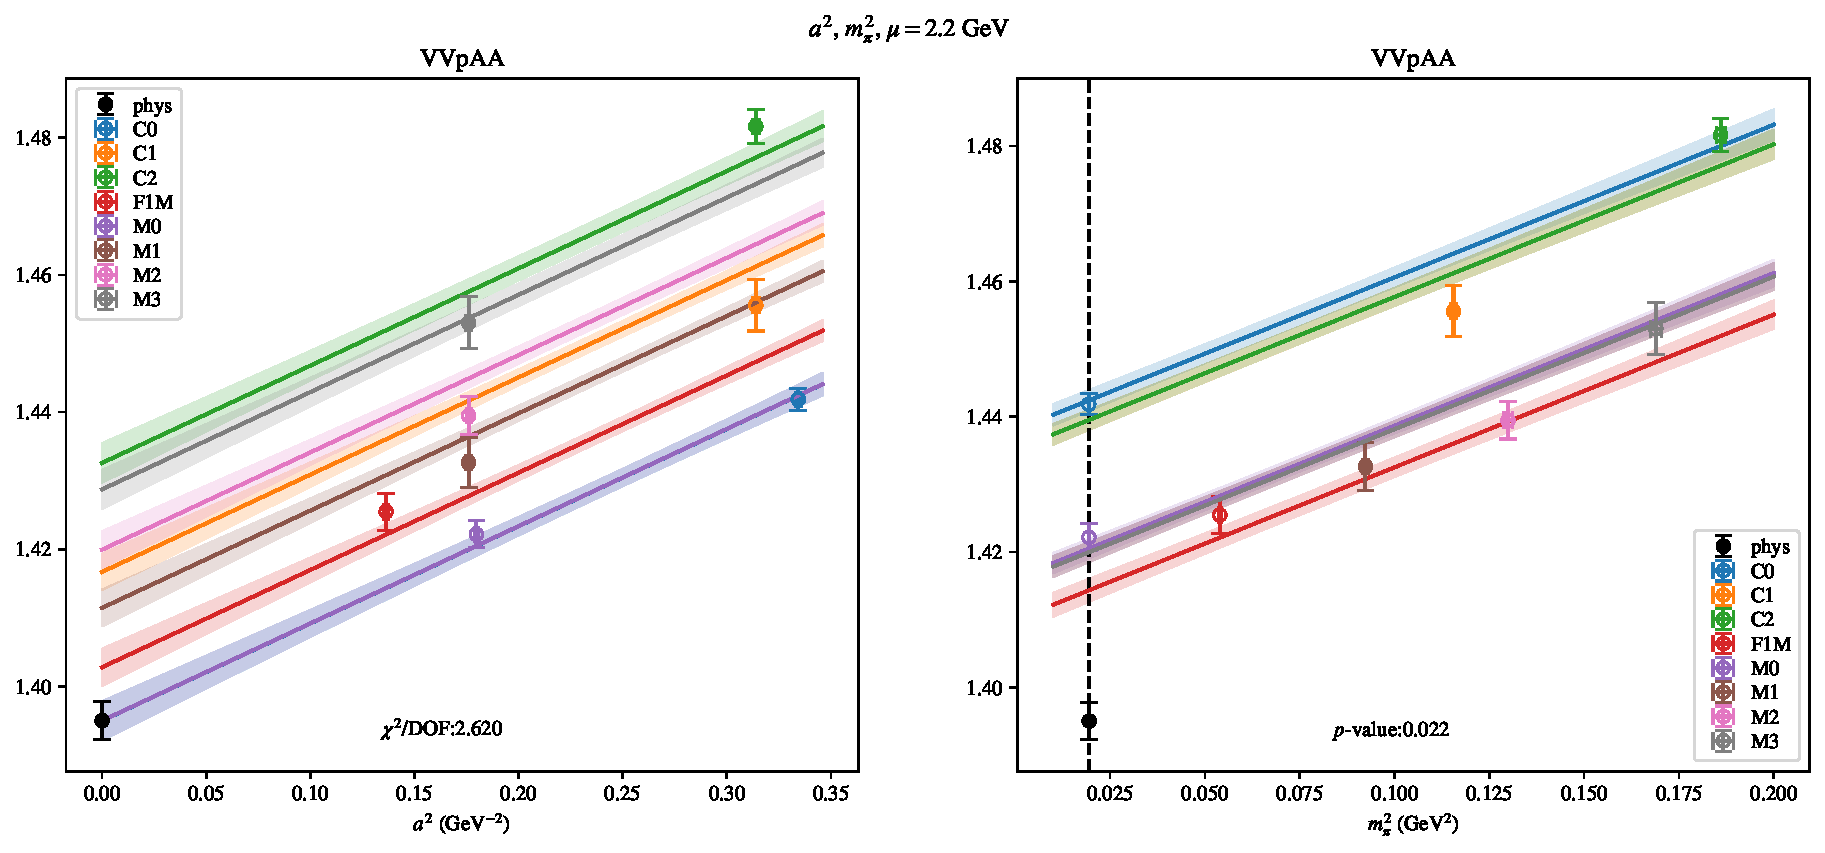
\includepdf[link, pages=-]{VVpAA/NPR/a2m2_22.pdf}
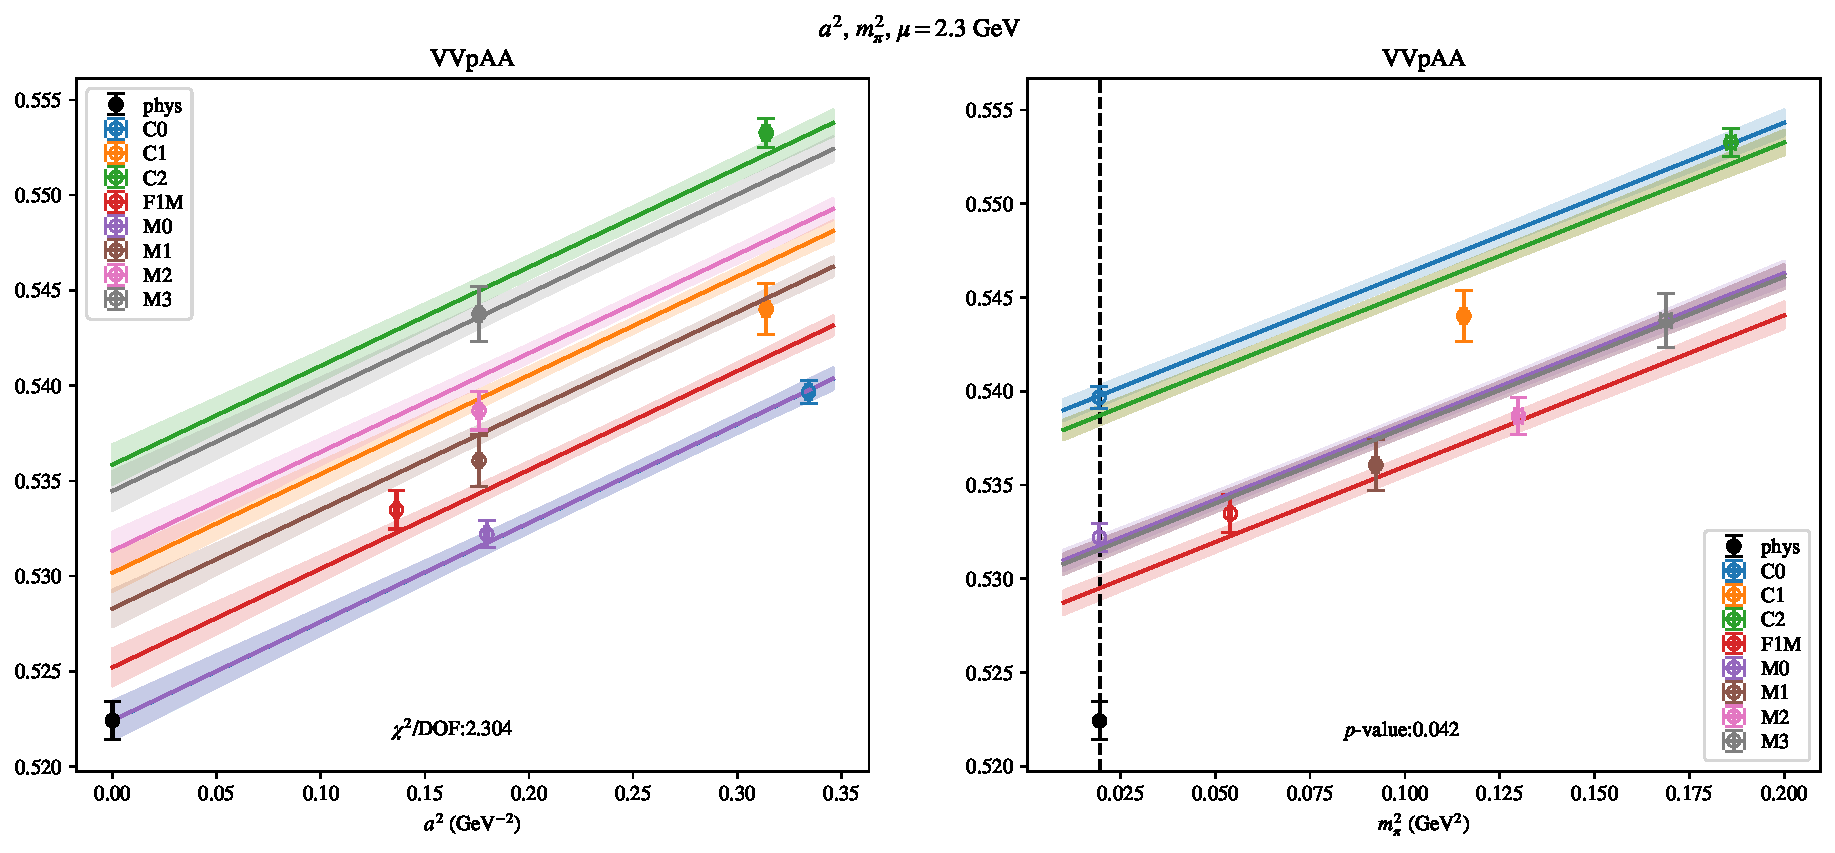
\includepdf[link, pages=-]{VVpAA/NPR/a2m2_23.pdf}
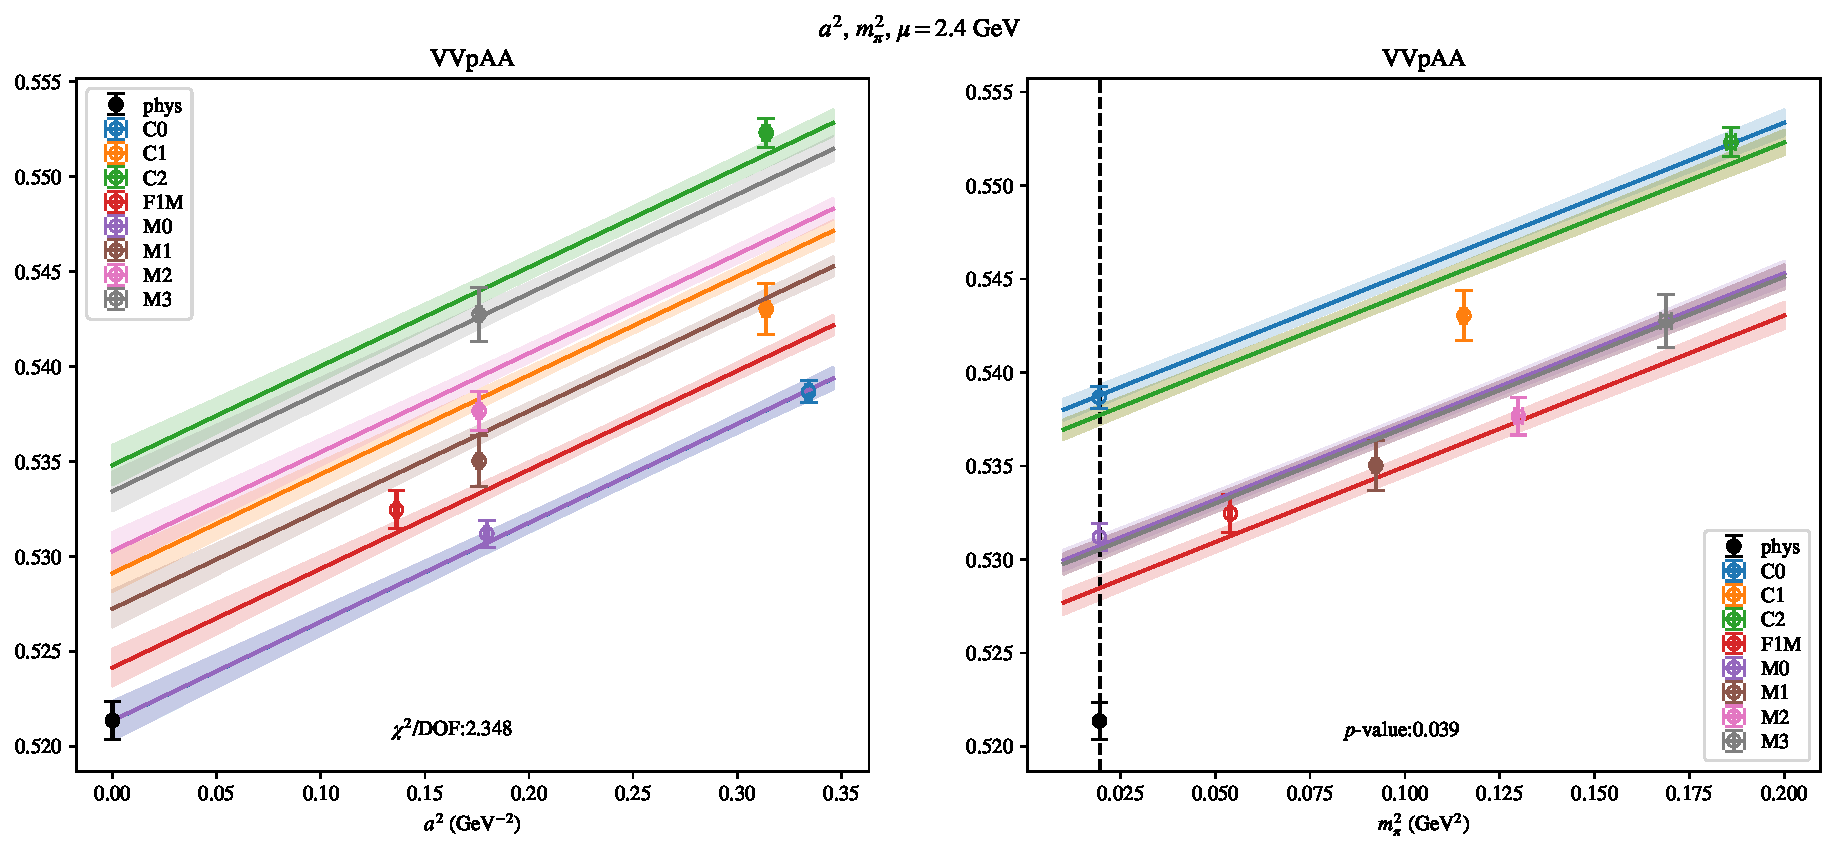
\includepdf[link, pages=-]{VVpAA/NPR/a2m2_24.pdf}
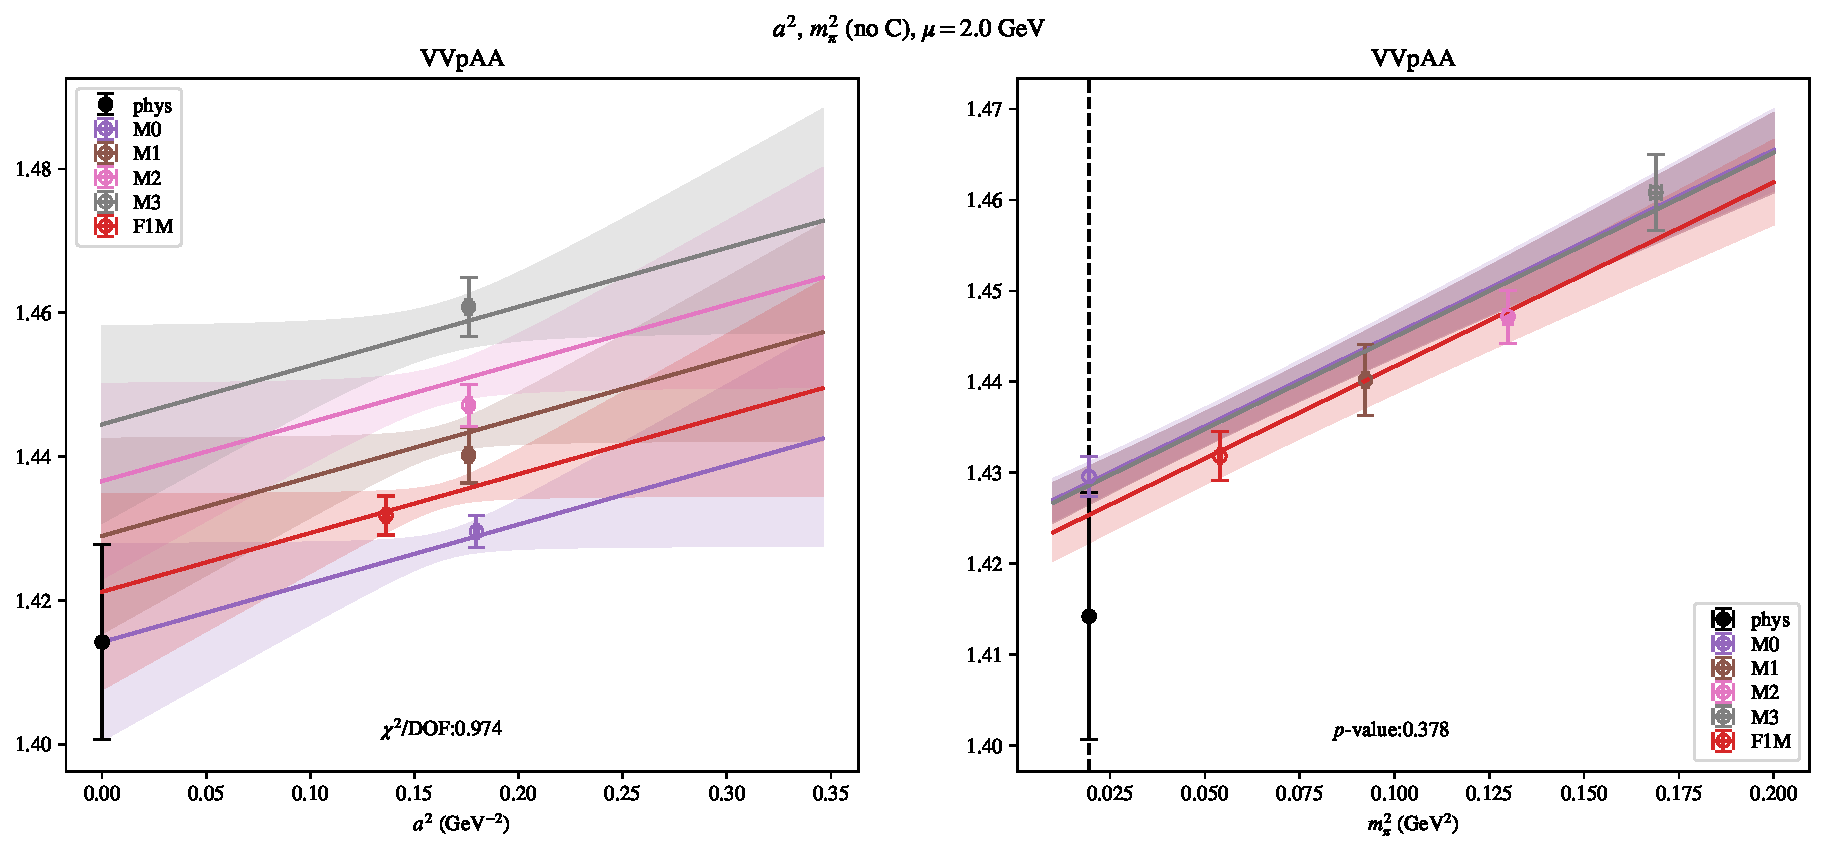
\includepdf[link, pages=-]{VVpAA/NPR/a2m2noC_20.pdf}
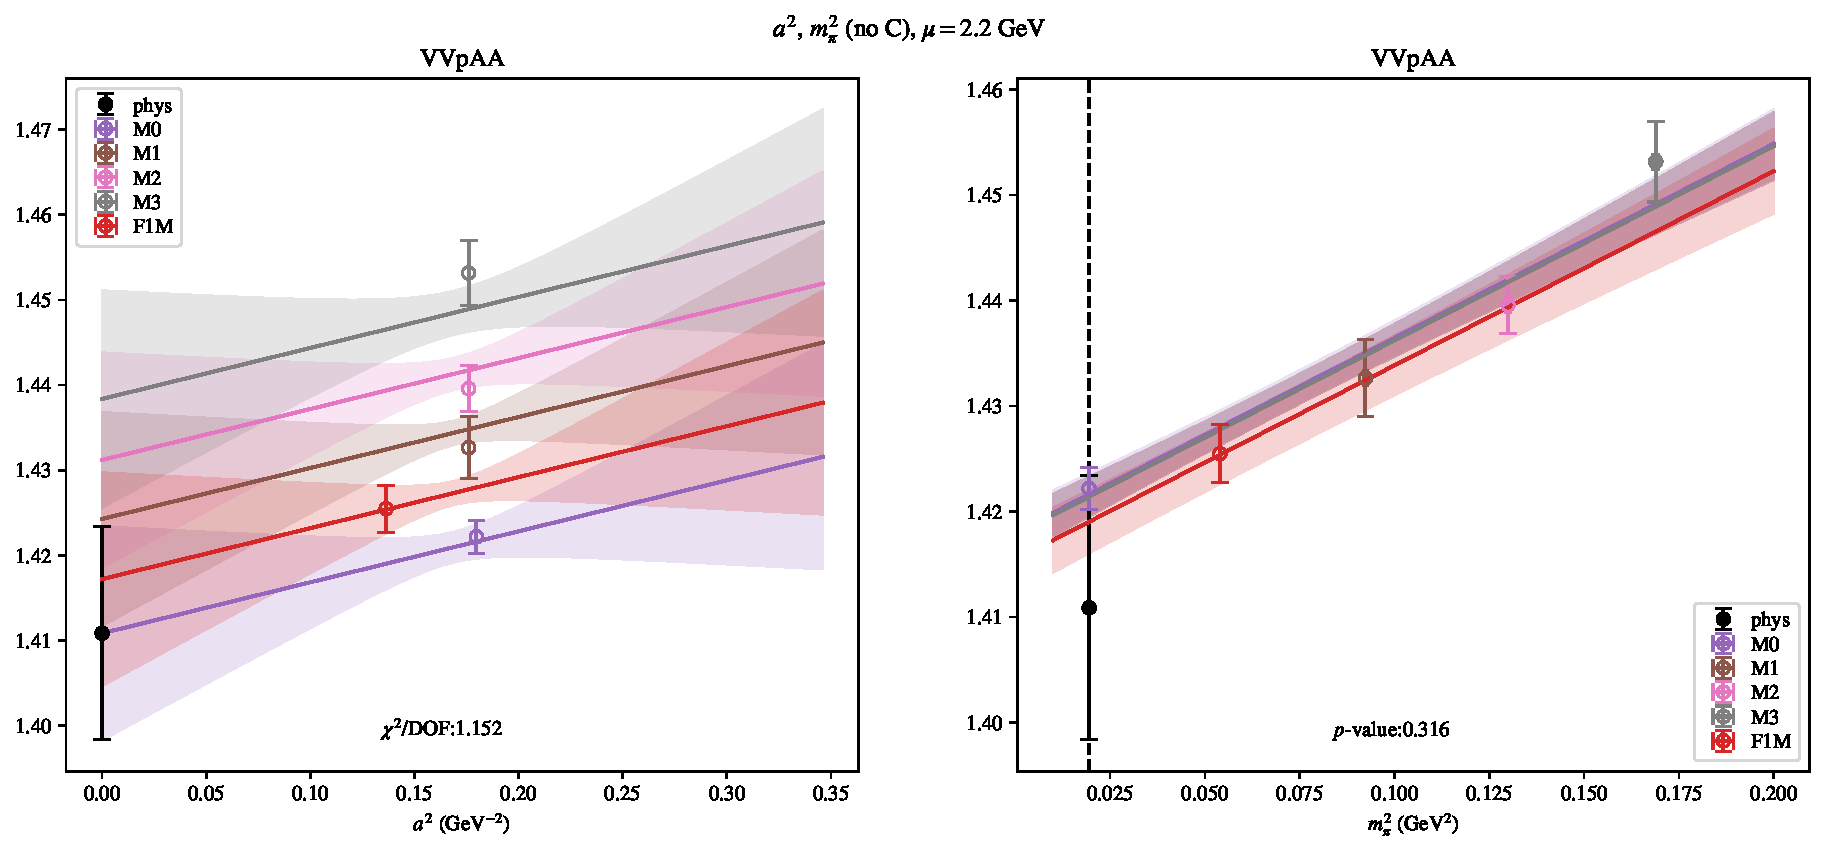
\includepdf[link, pages=-]{VVpAA/NPR/a2m2noC_22.pdf}
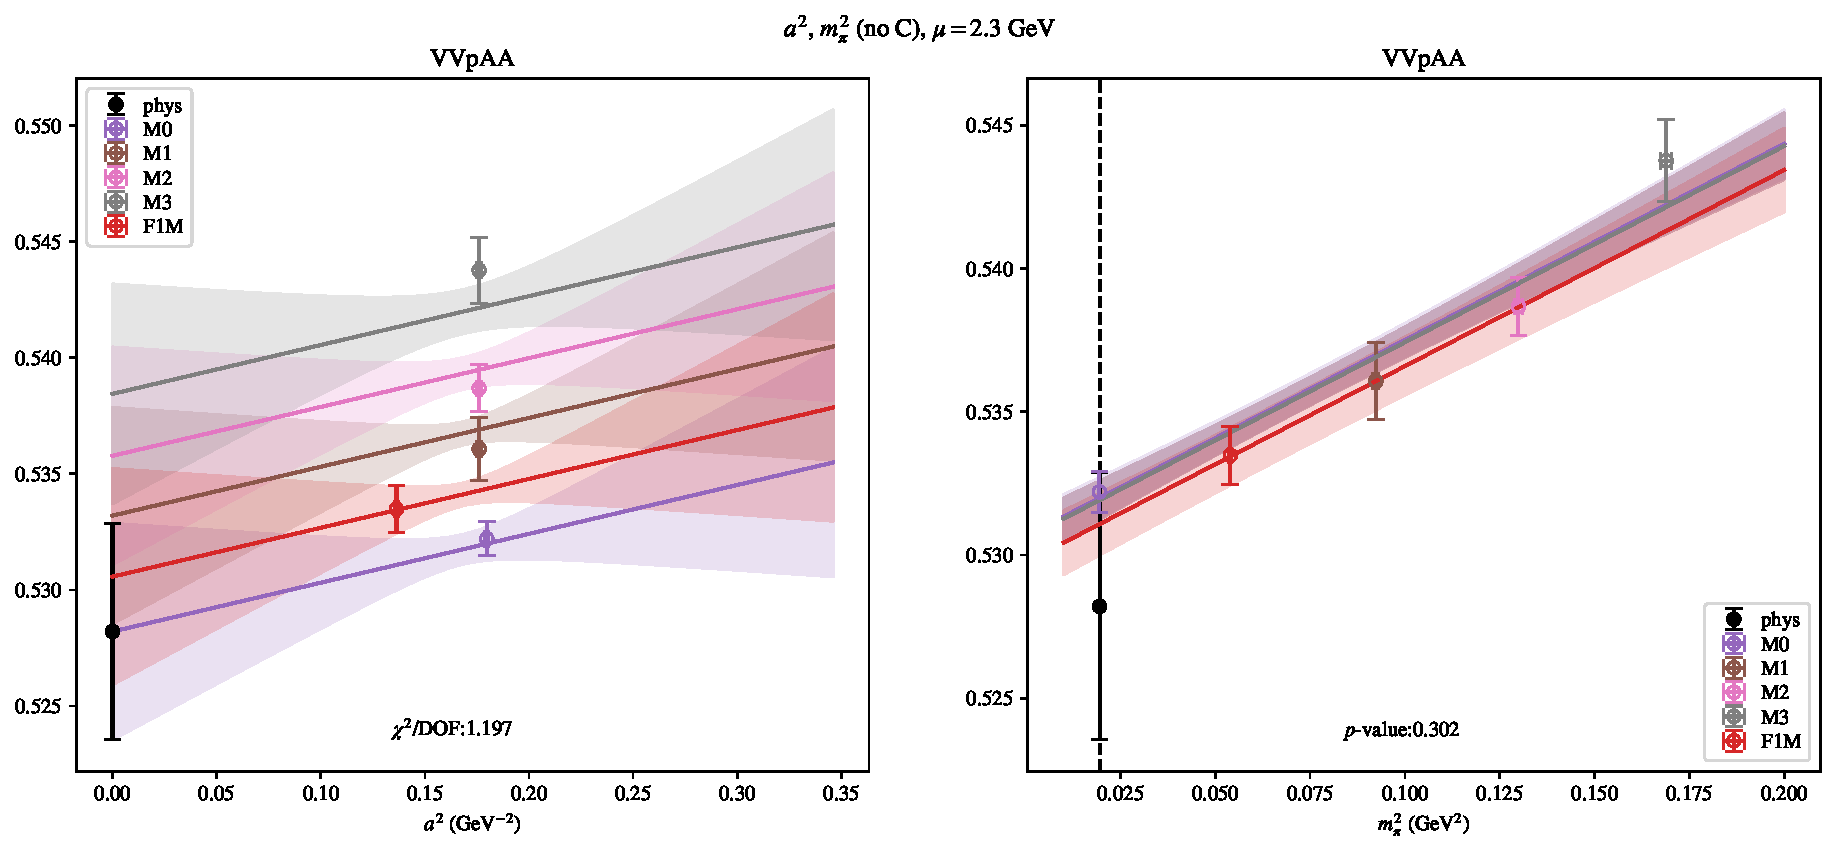
\includepdf[link, pages=-]{VVpAA/NPR/a2m2noC_23.pdf}
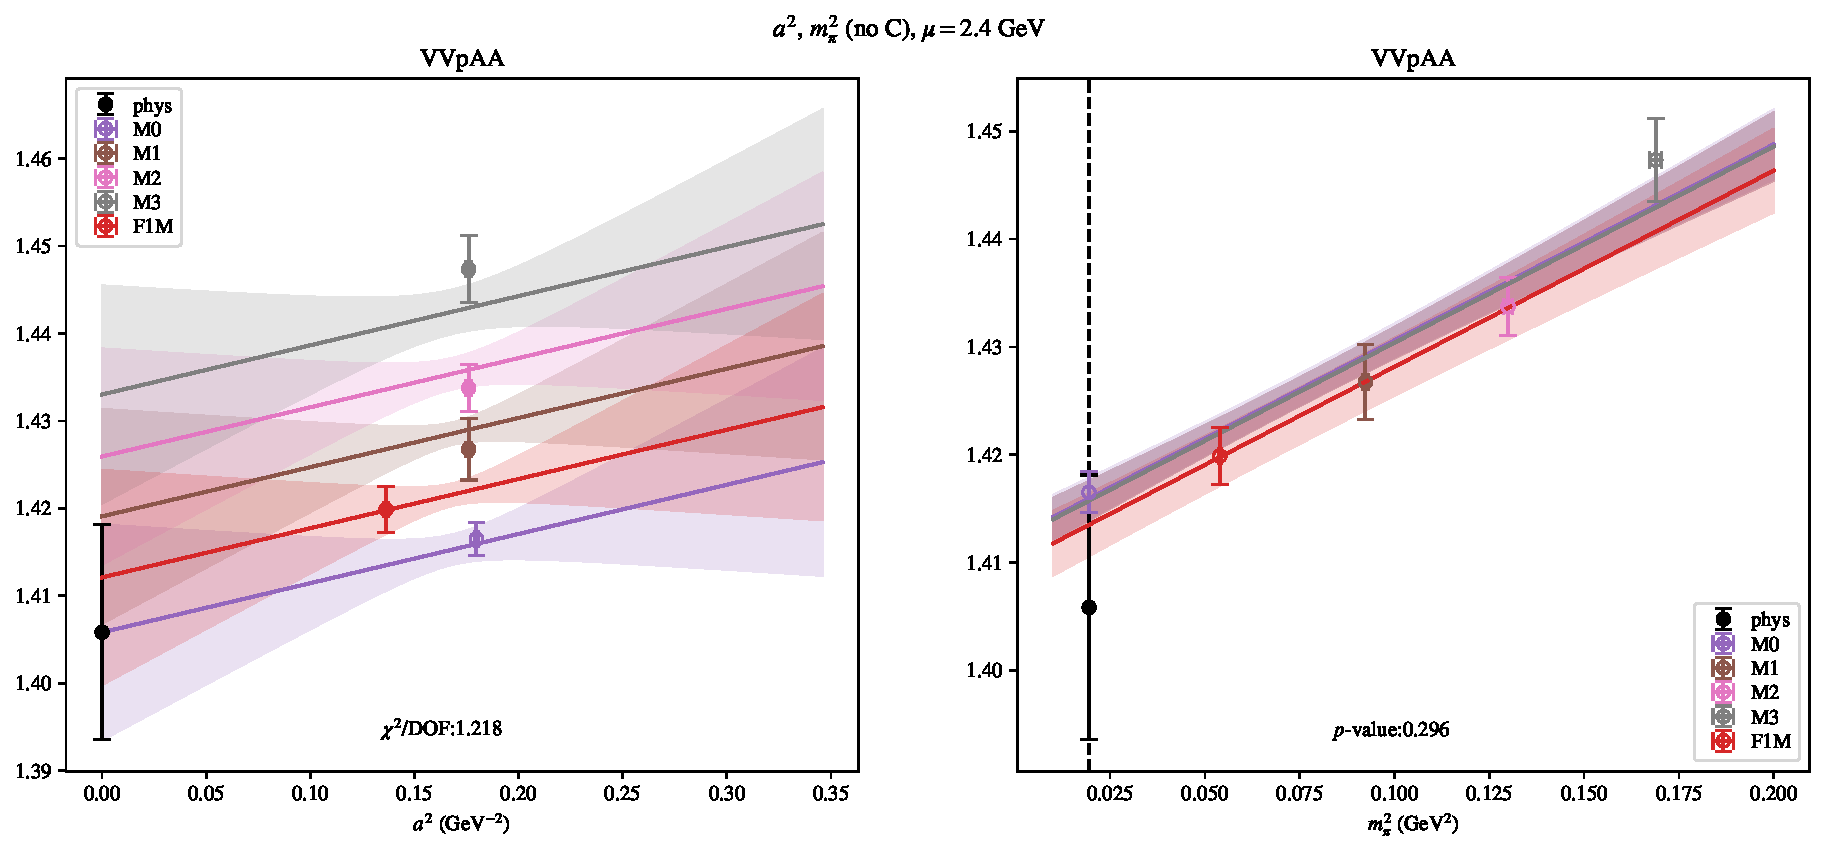
\includepdf[link, pages=-]{VVpAA/NPR/a2m2noC_24.pdf}
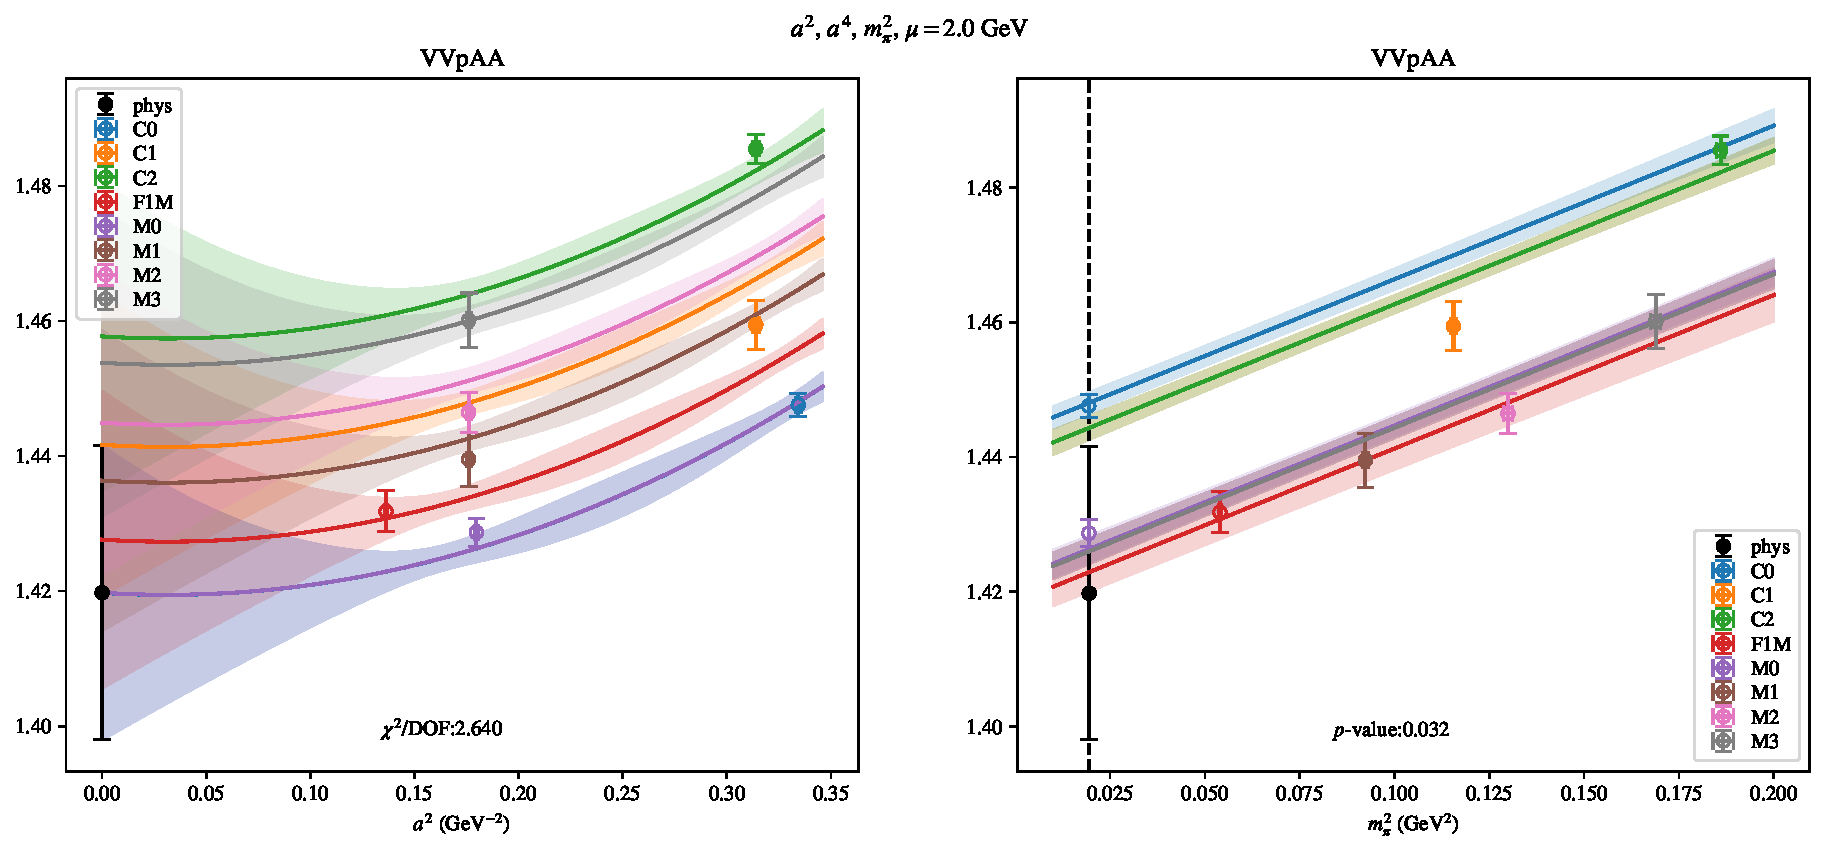
\includepdf[link, pages=-]{VVpAA/NPR/a2a4m2_20.pdf}
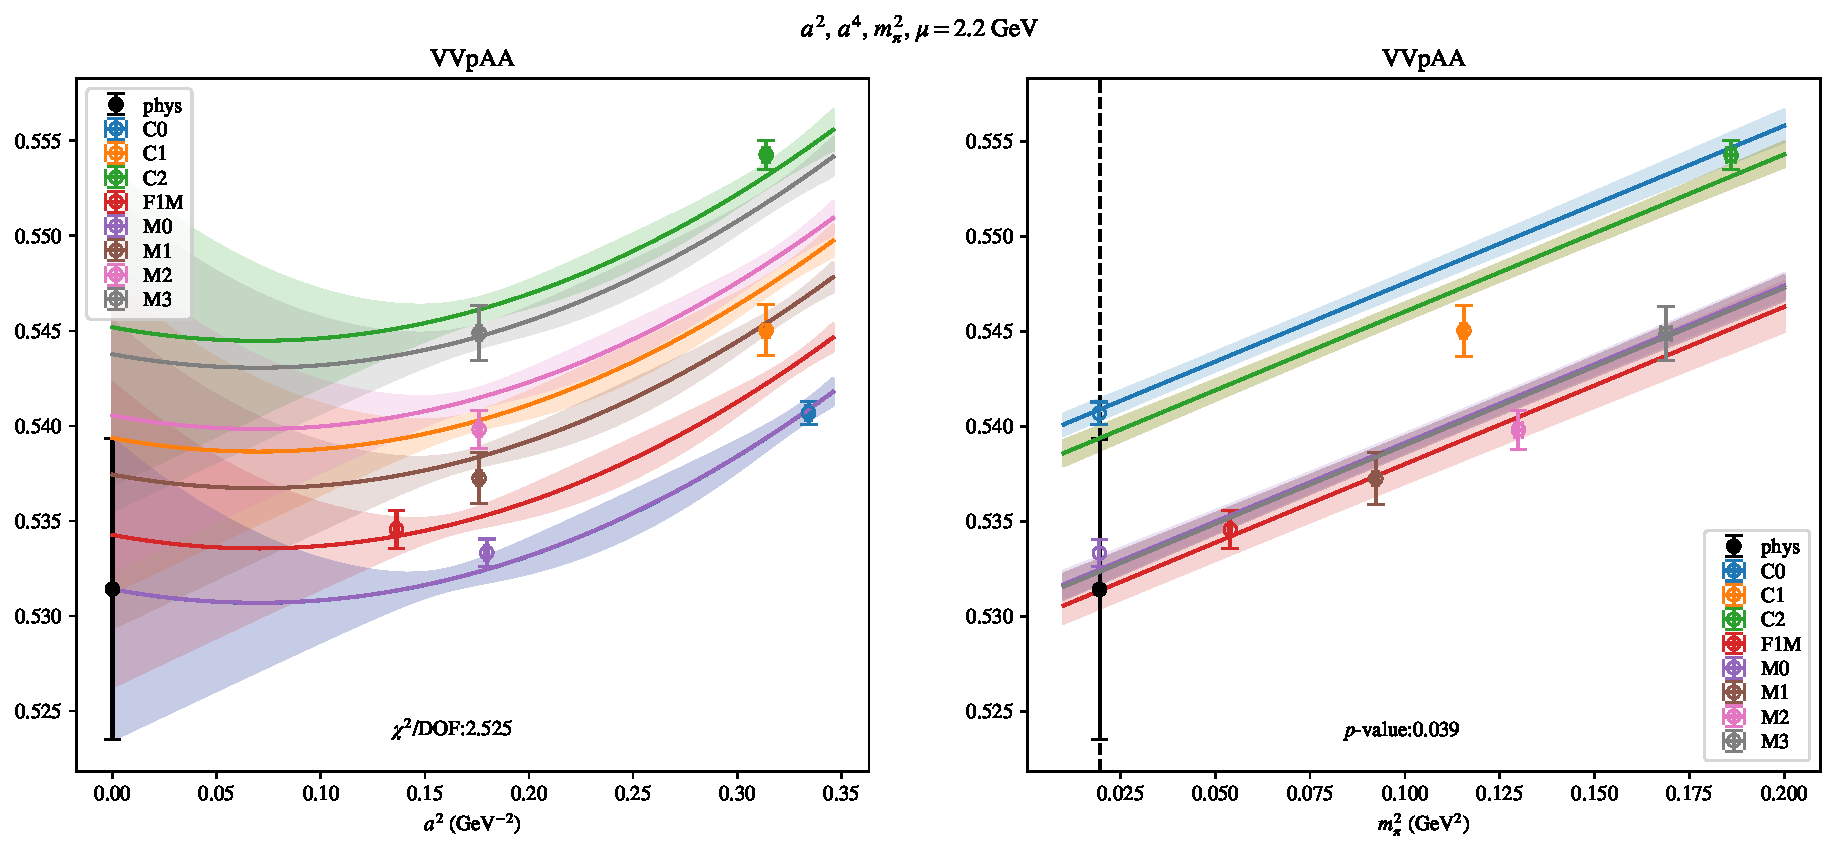
\includepdf[link, pages=-]{VVpAA/NPR/a2a4m2_22.pdf}
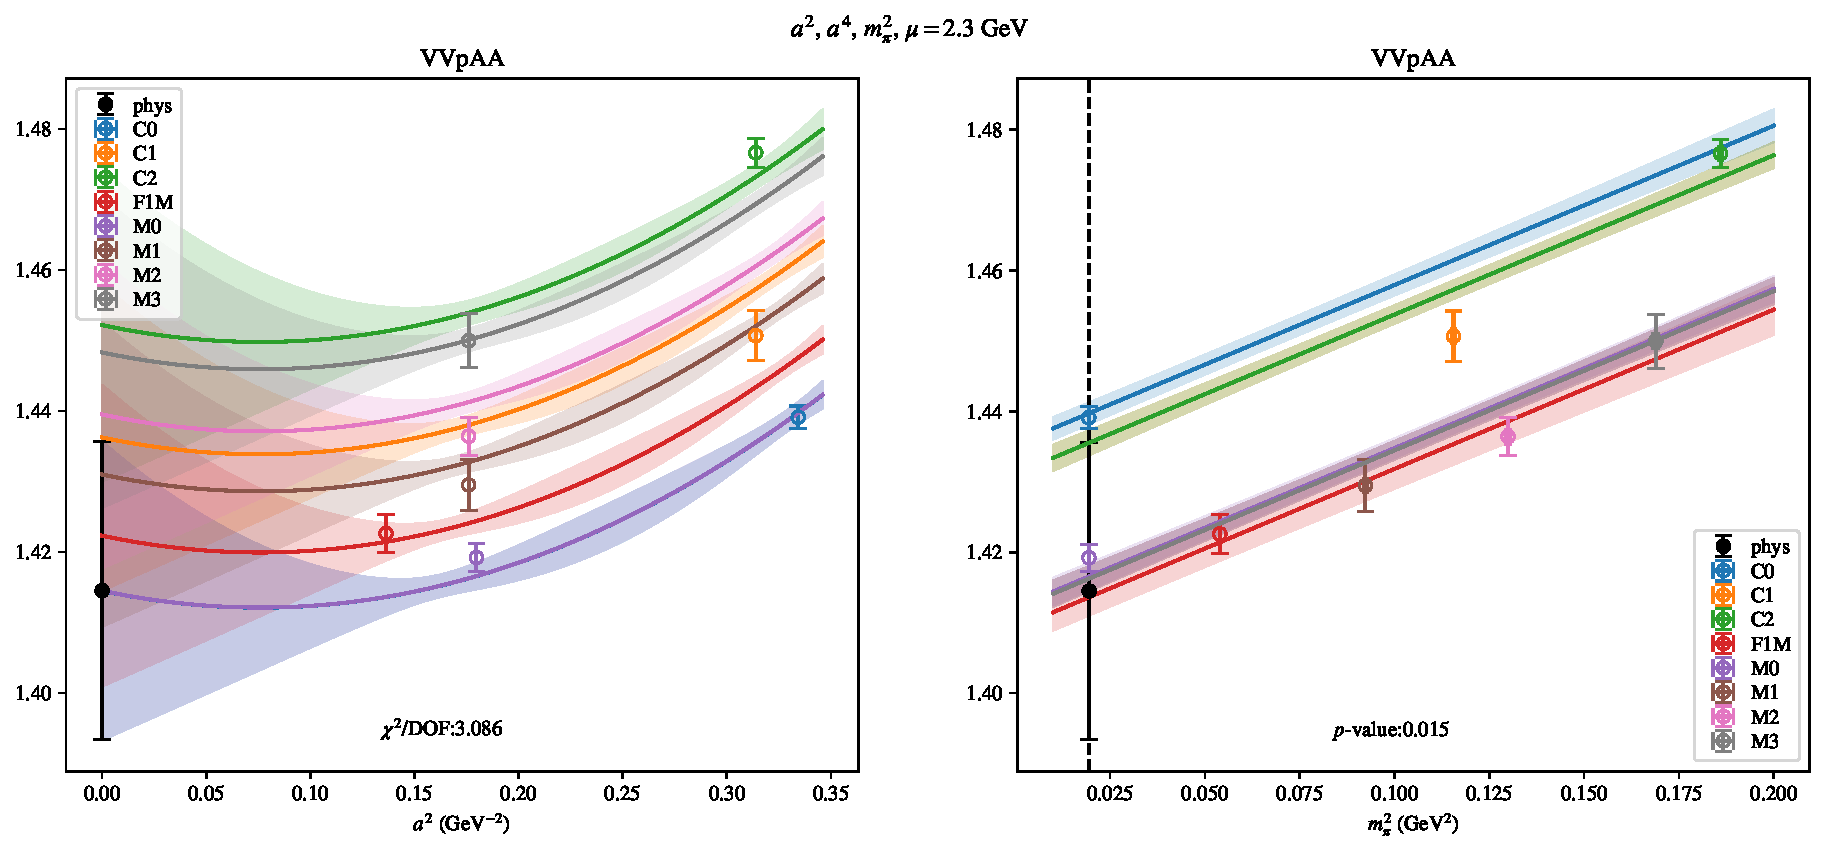
\includepdf[link, pages=-]{VVpAA/NPR/a2a4m2_23.pdf}
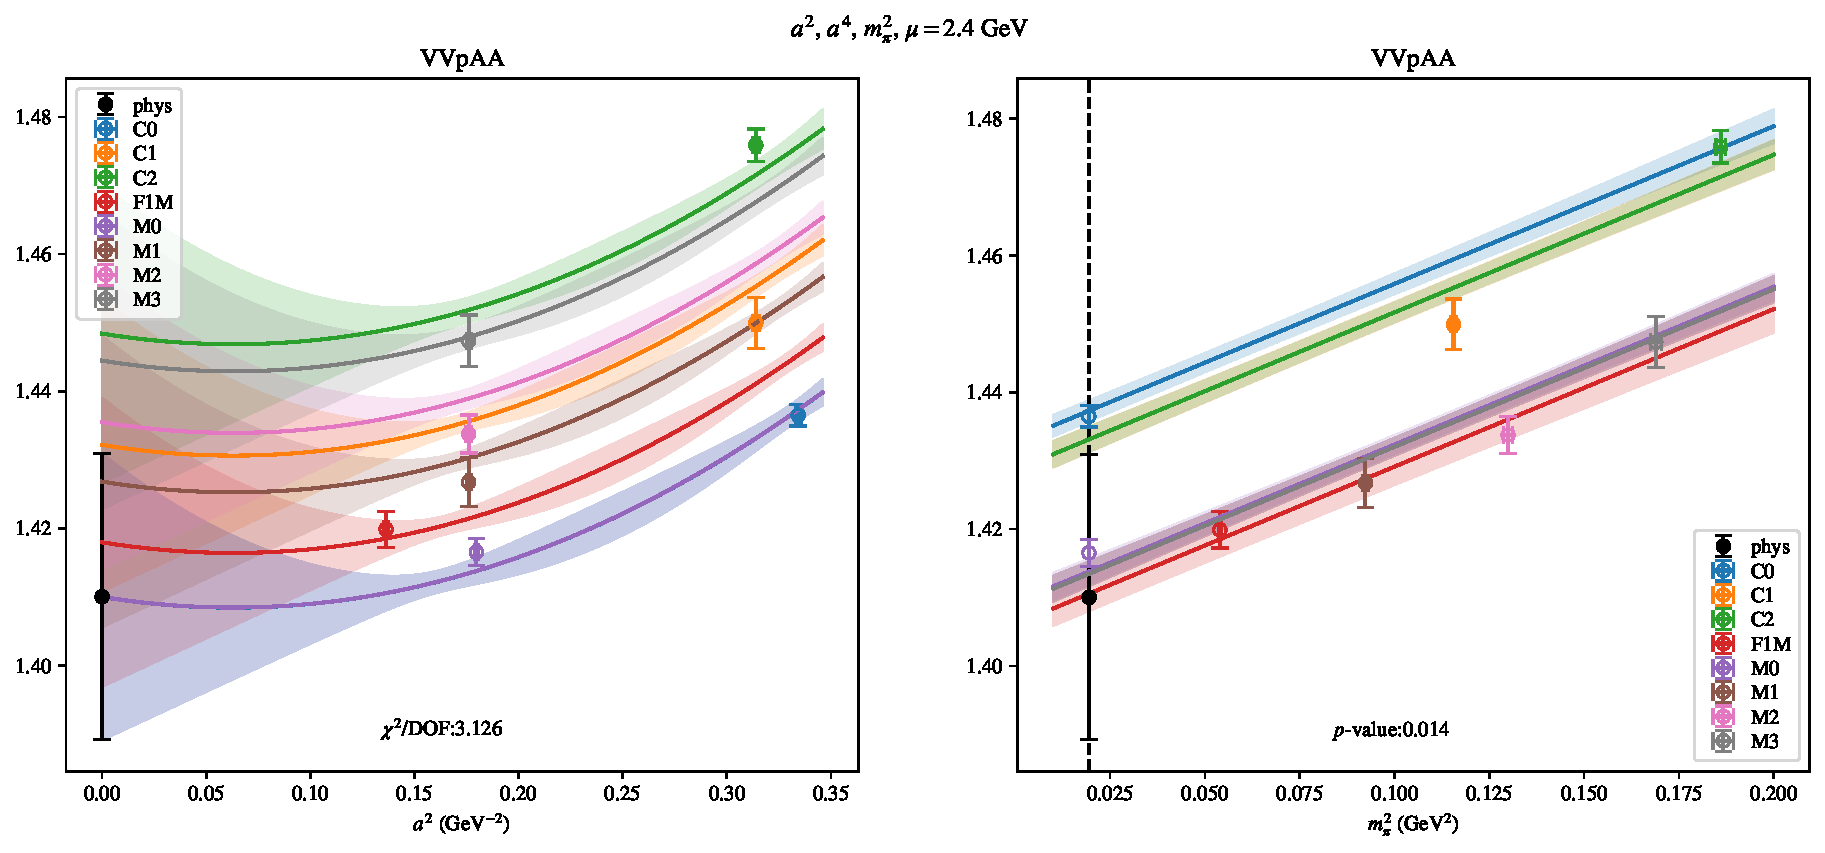
\includepdf[link, pages=-]{VVpAA/NPR/a2a4m2_24.pdf}
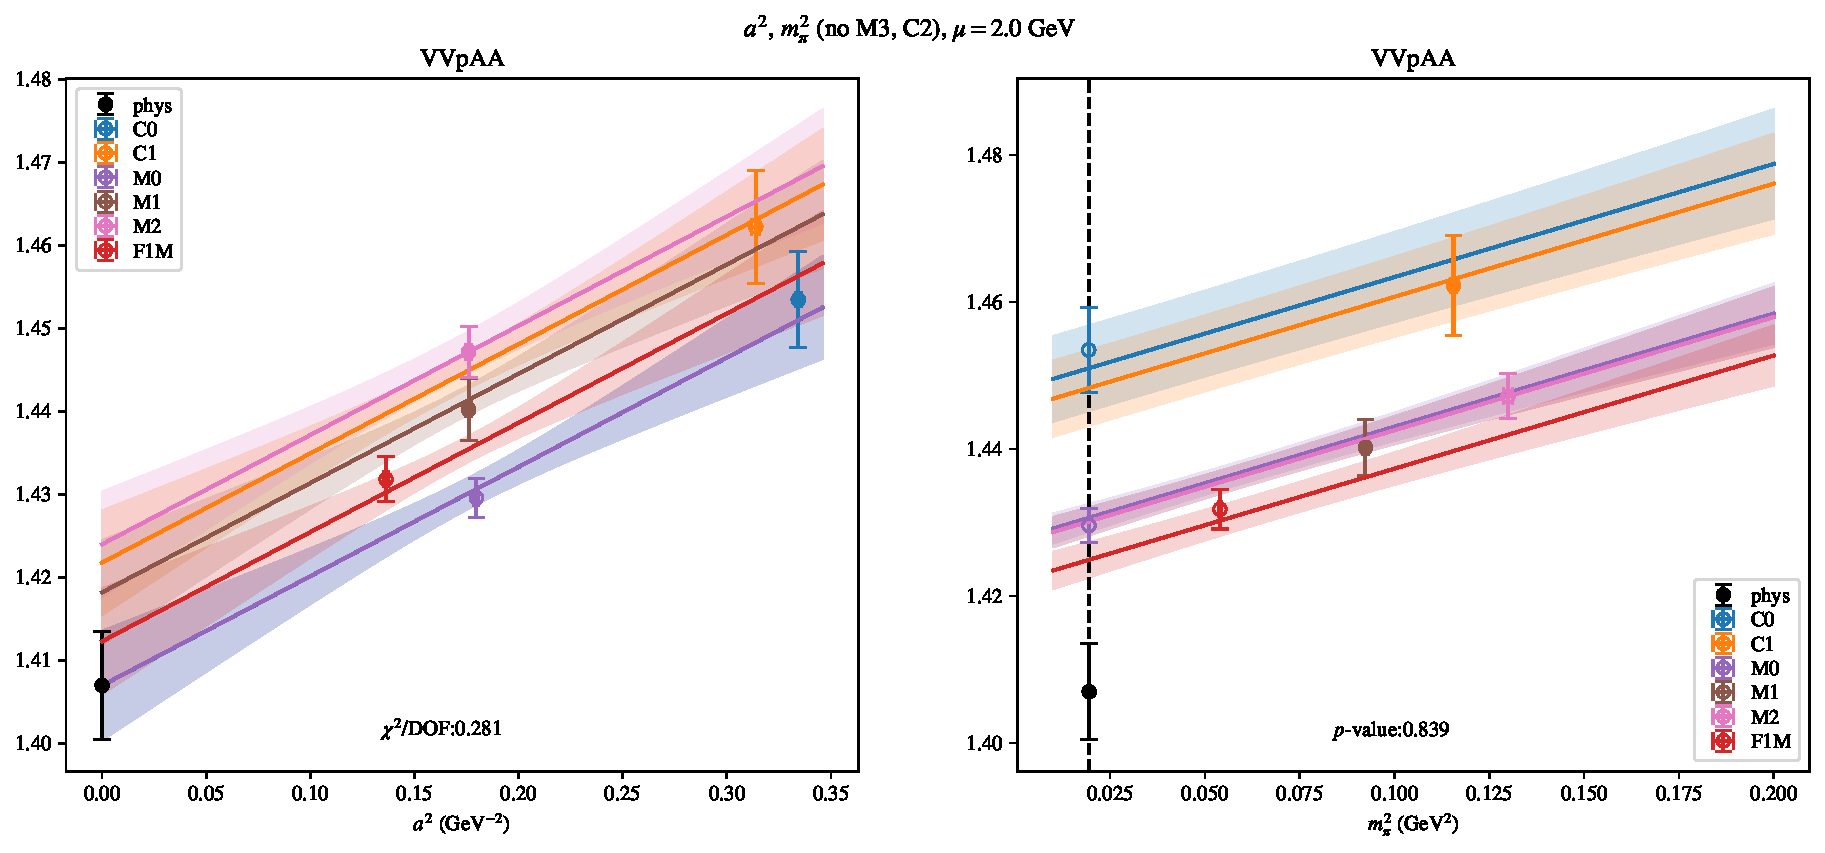
\includepdf[link, pages=-]{VVpAA/NPR/a2m2mcut_20.pdf}
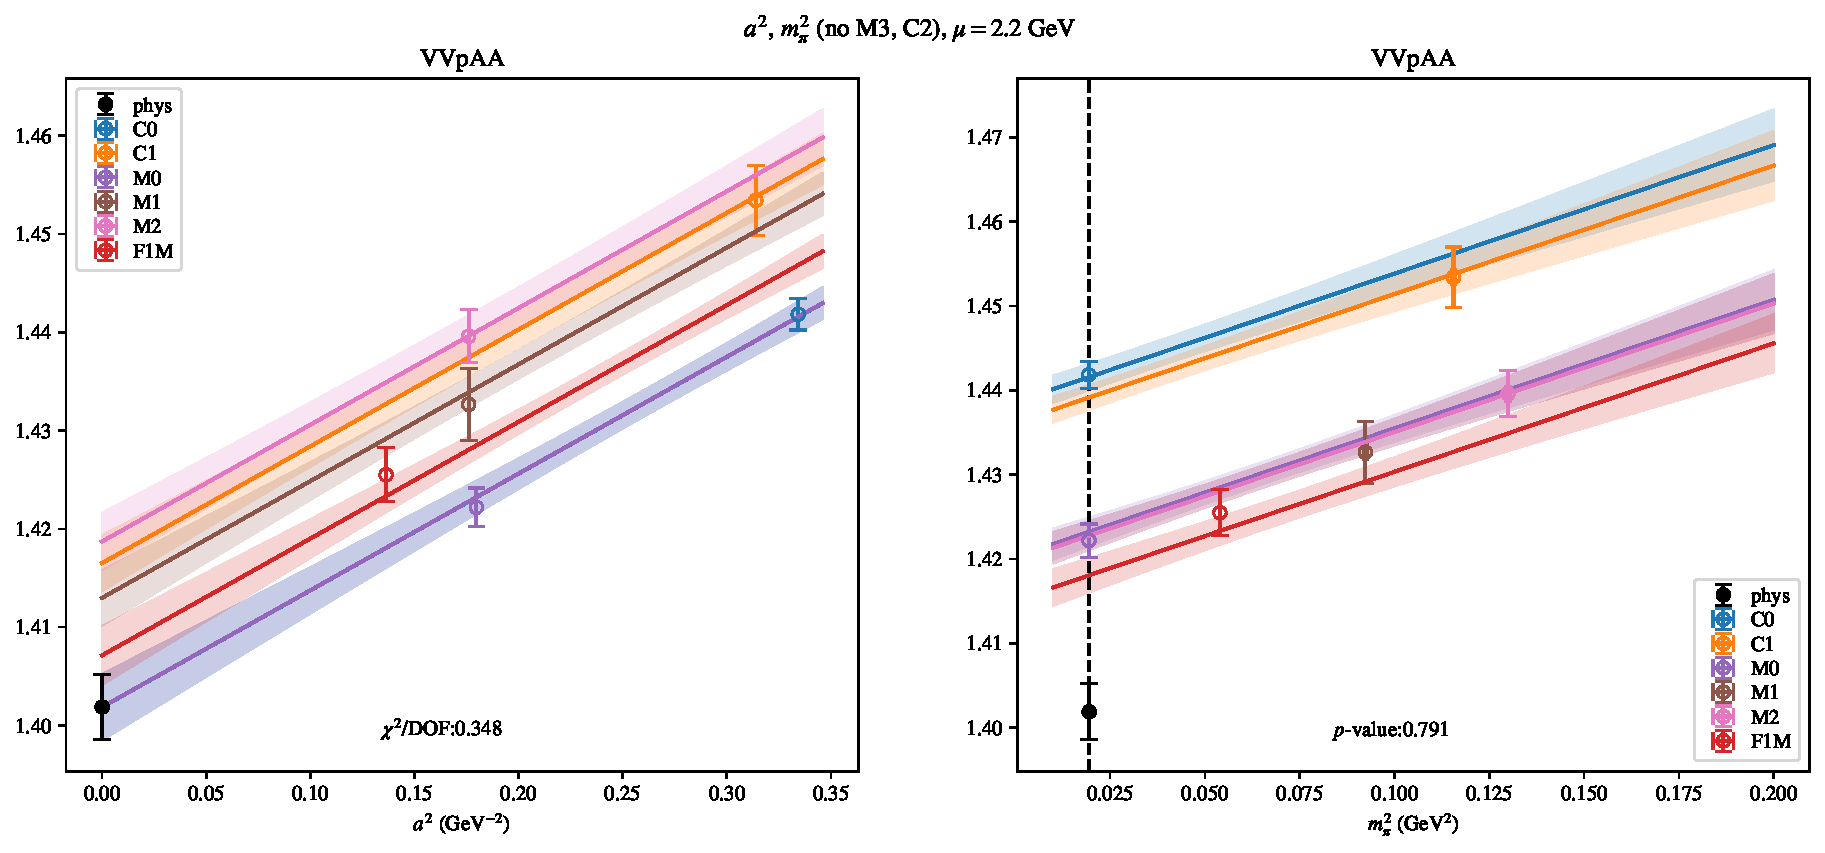
\includepdf[link, pages=-]{VVpAA/NPR/a2m2mcut_22.pdf}
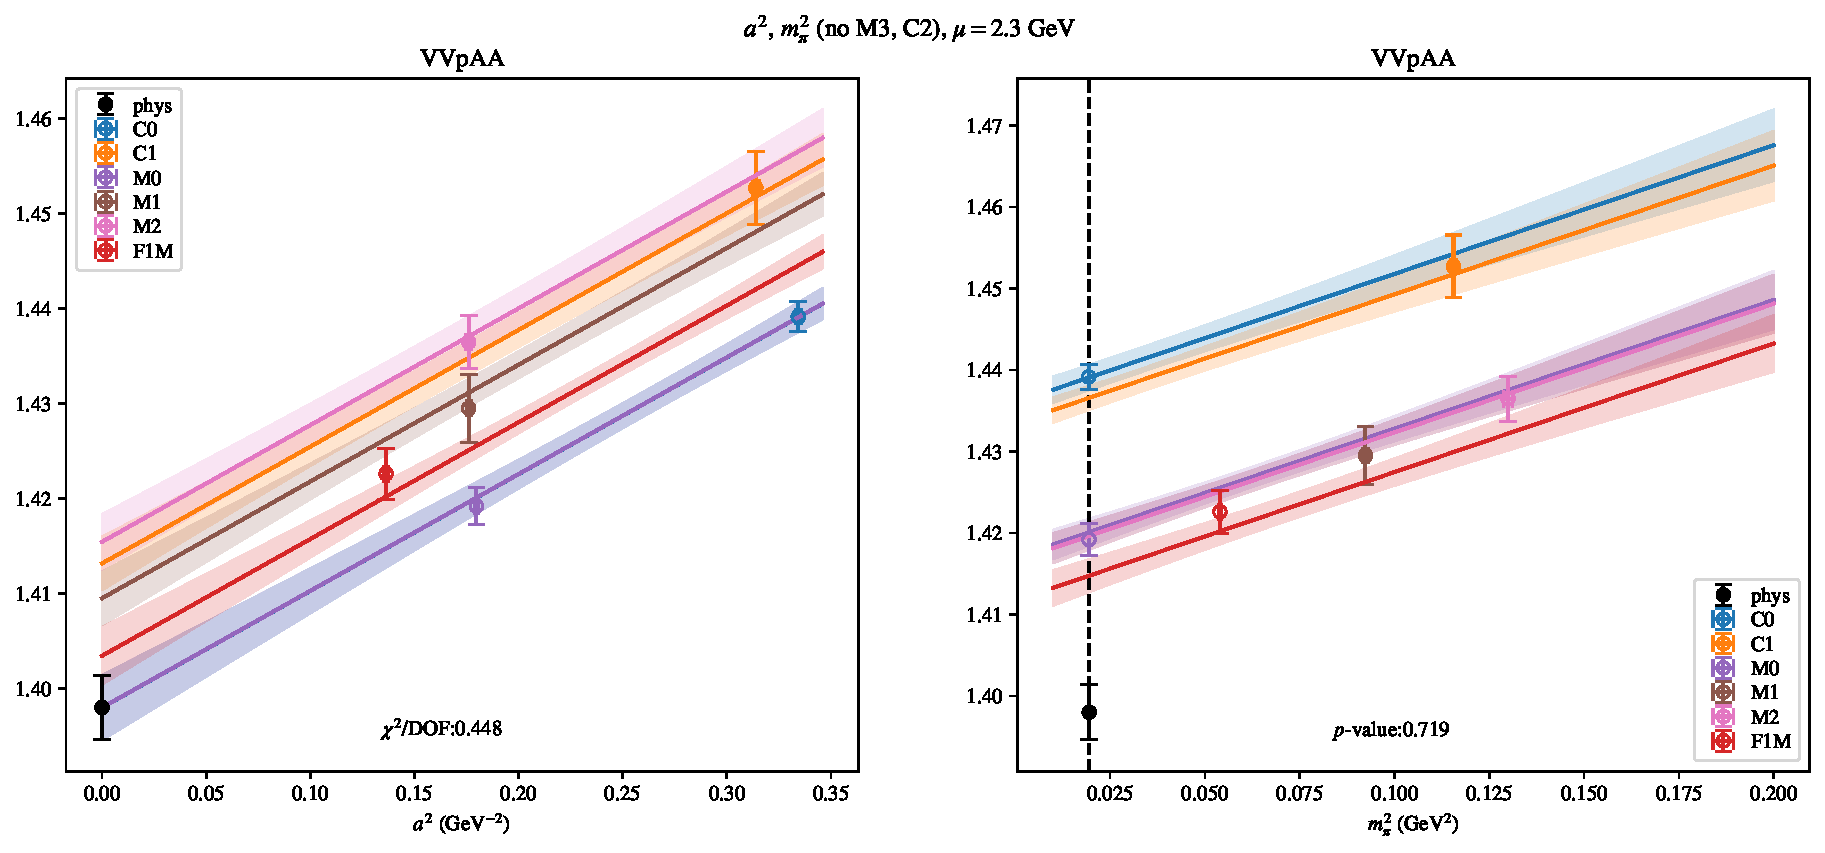
\includepdf[link, pages=-]{VVpAA/NPR/a2m2mcut_23.pdf}
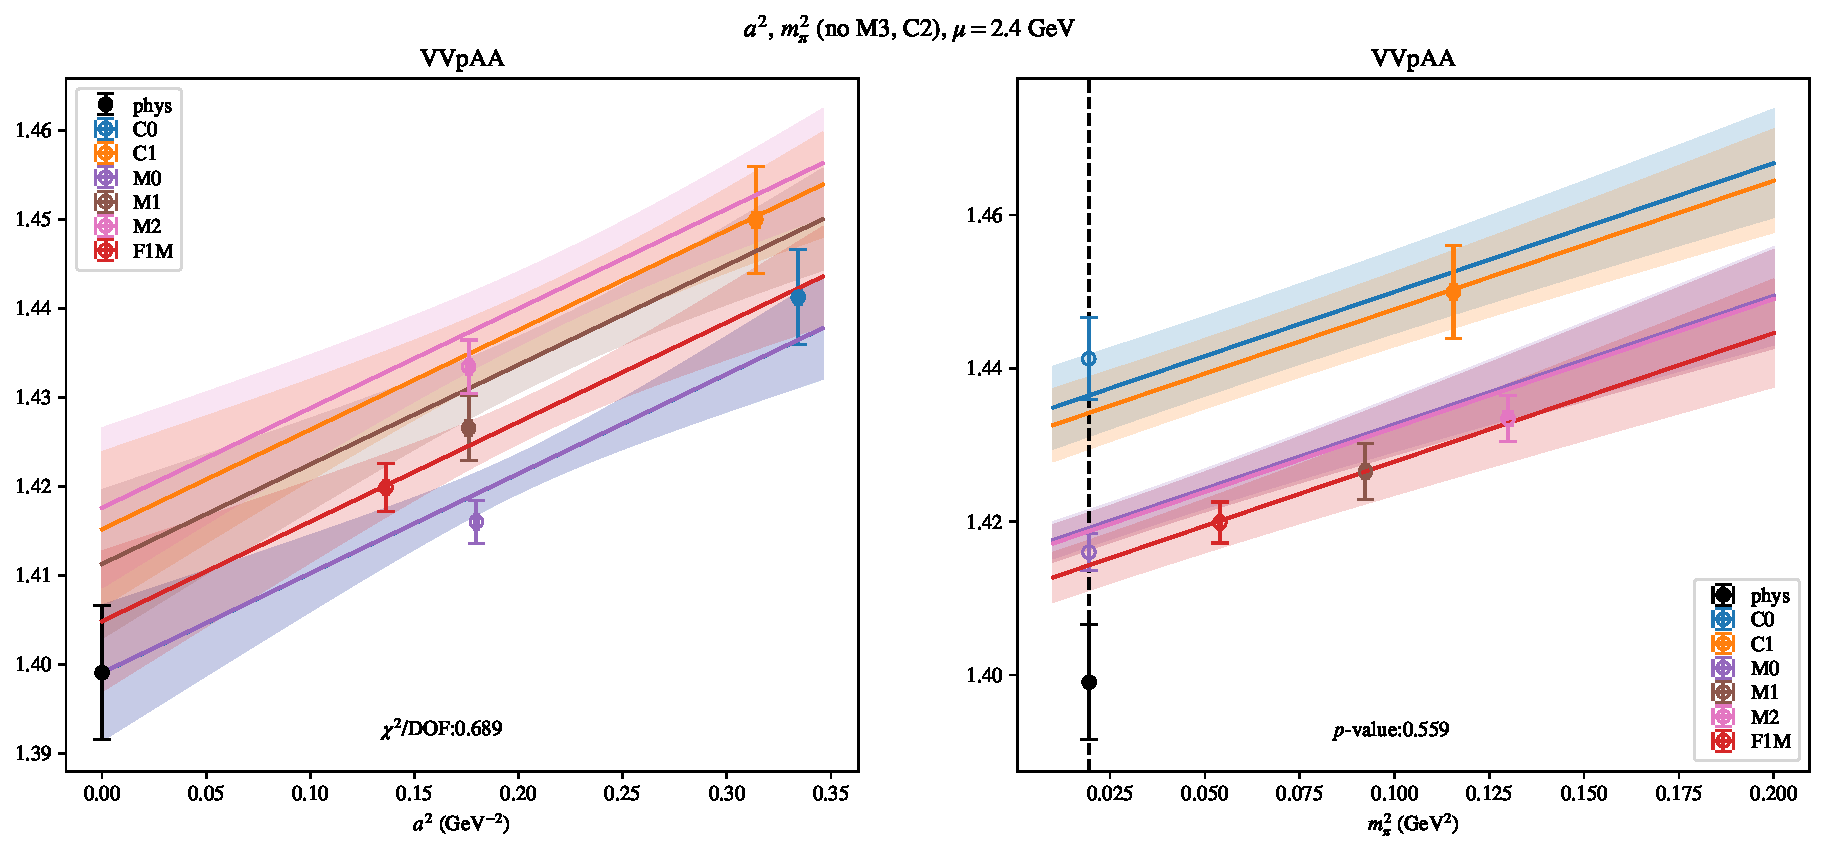
\includepdf[link, pages=-]{VVpAA/NPR/a2m2mcut_24.pdf}
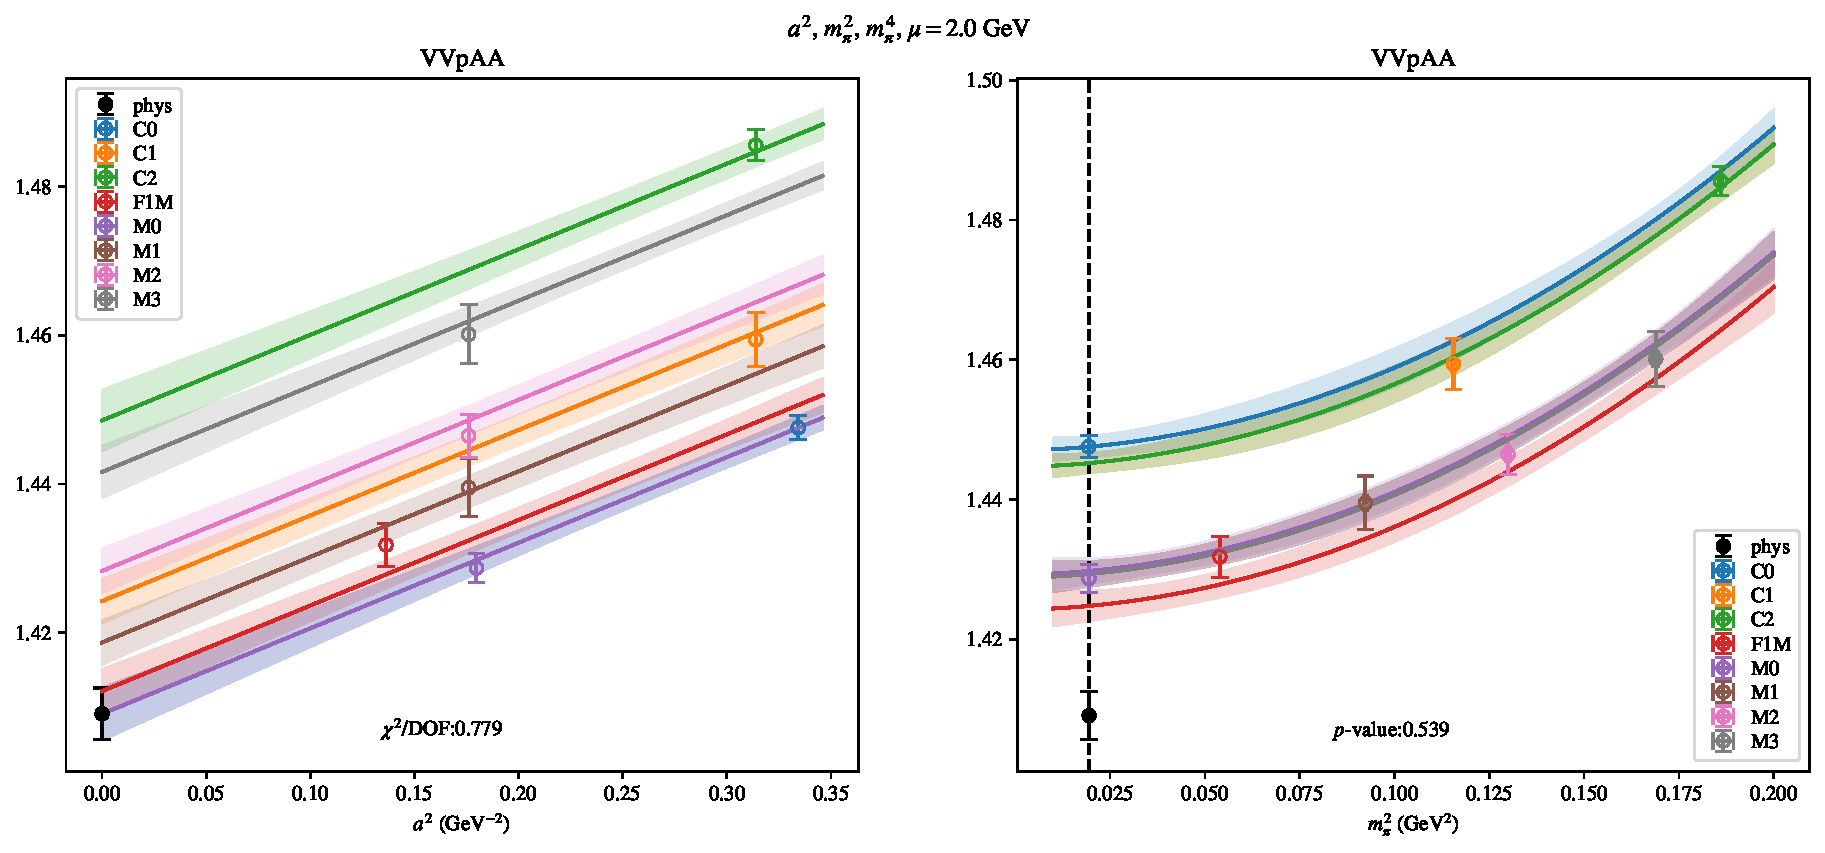
\includepdf[link, pages=-]{VVpAA/NPR/a2m2m4_20.pdf}
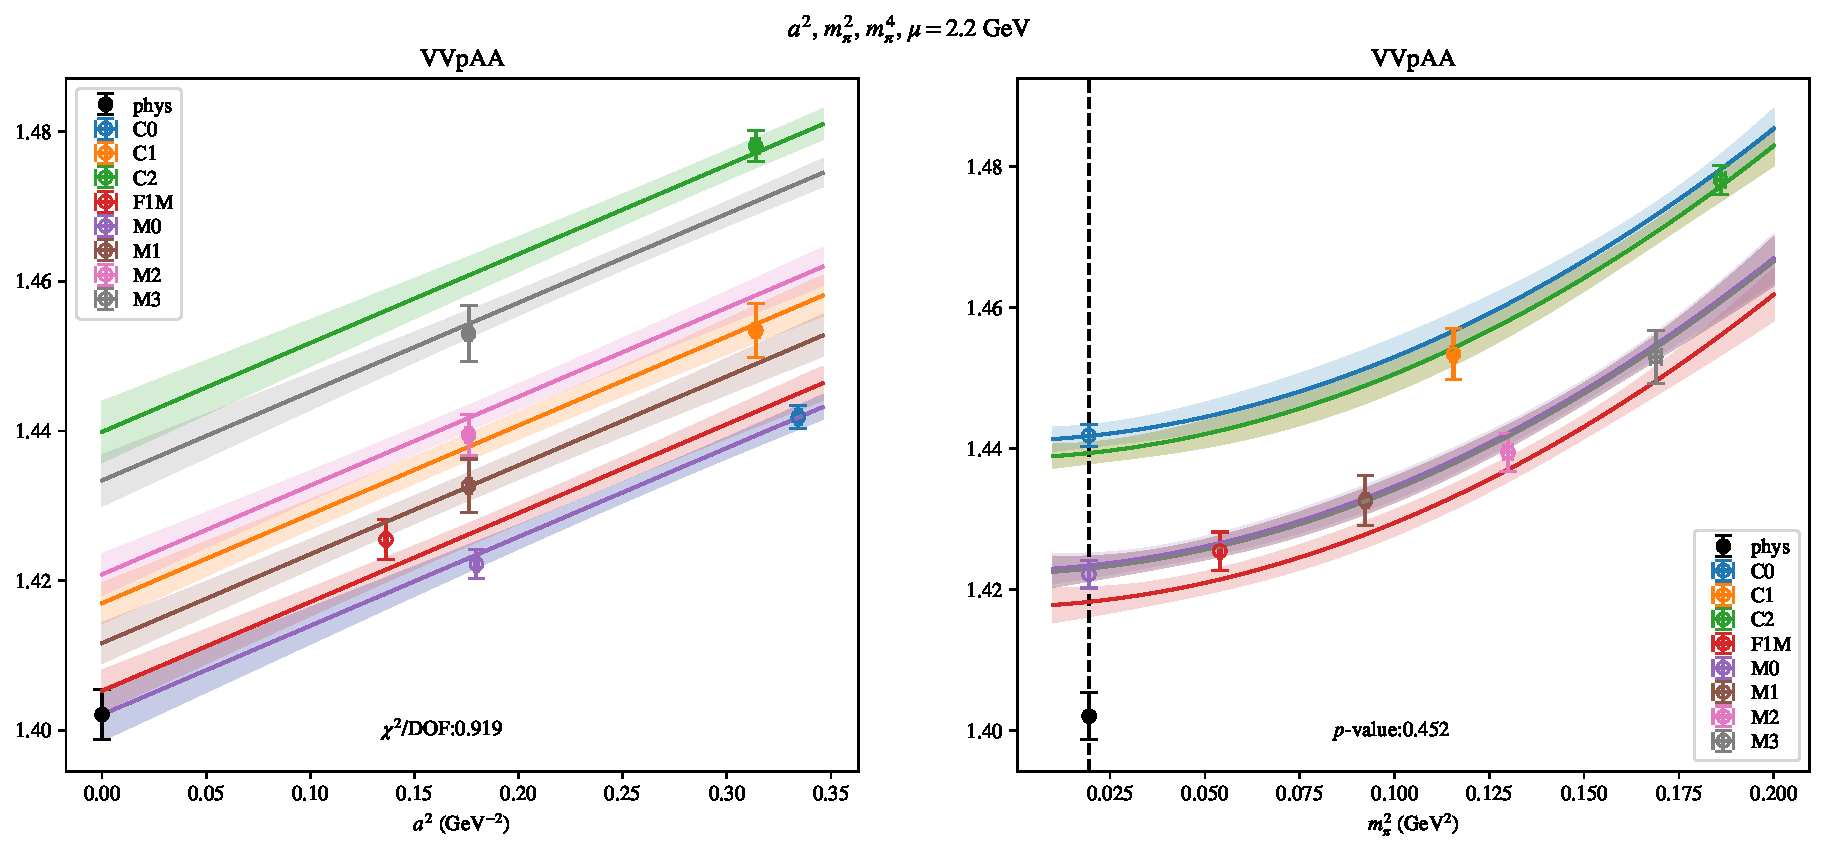
\includepdf[link, pages=-]{VVpAA/NPR/a2m2m4_22.pdf}
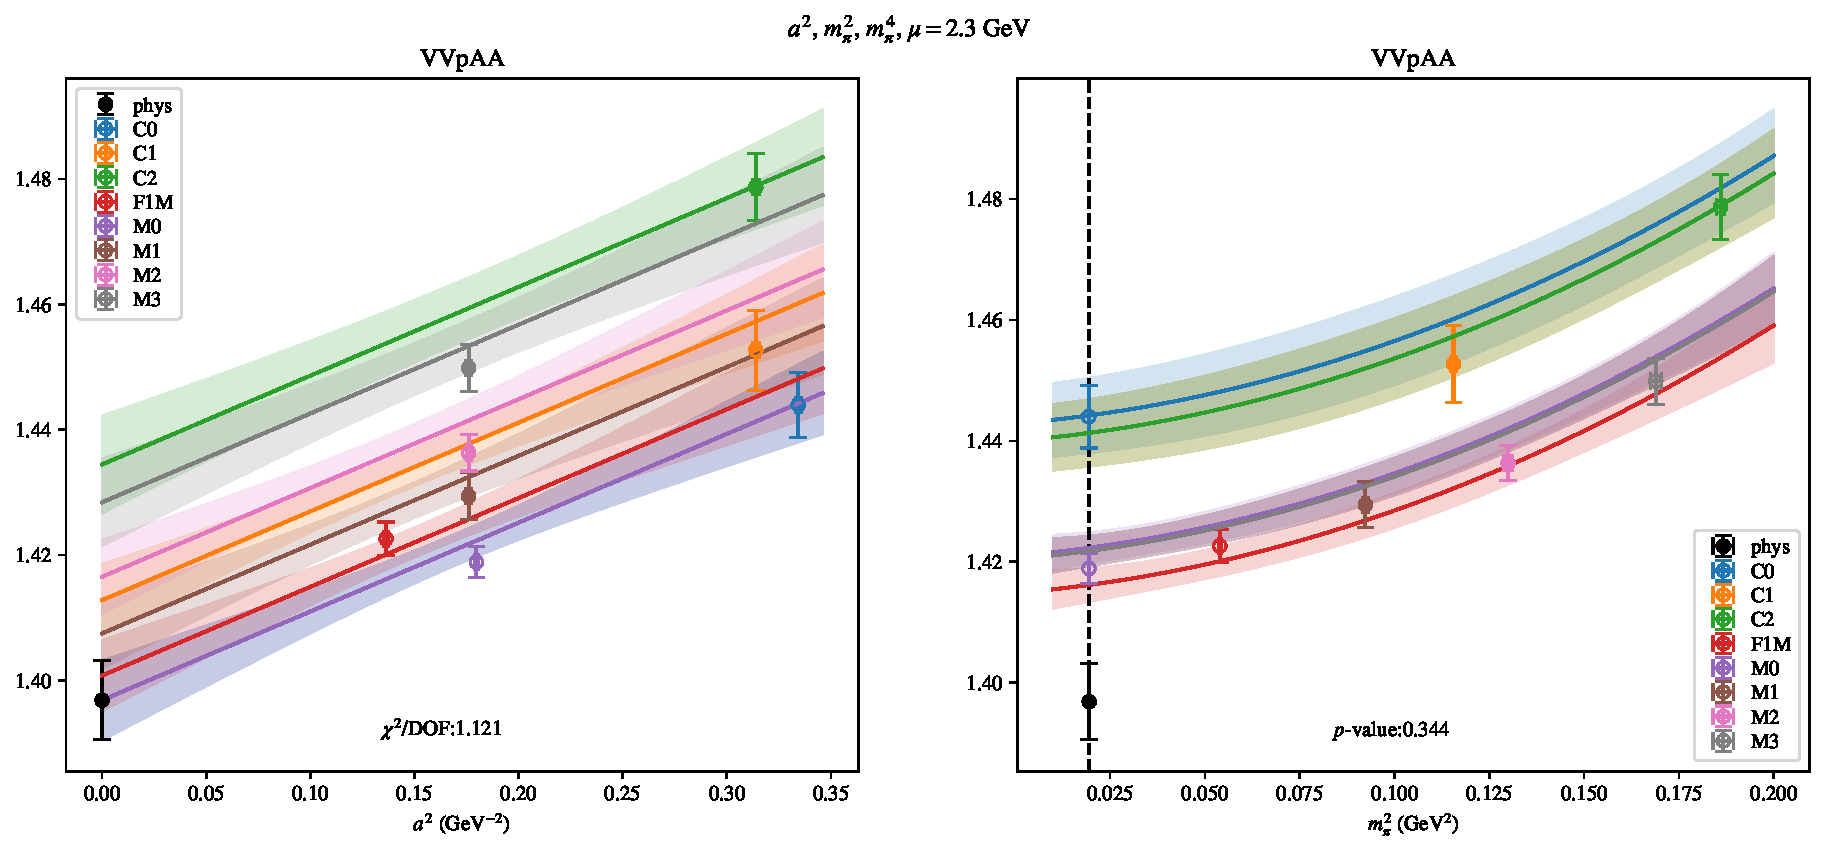
\includepdf[link, pages=-]{VVpAA/NPR/a2m2m4_23.pdf}
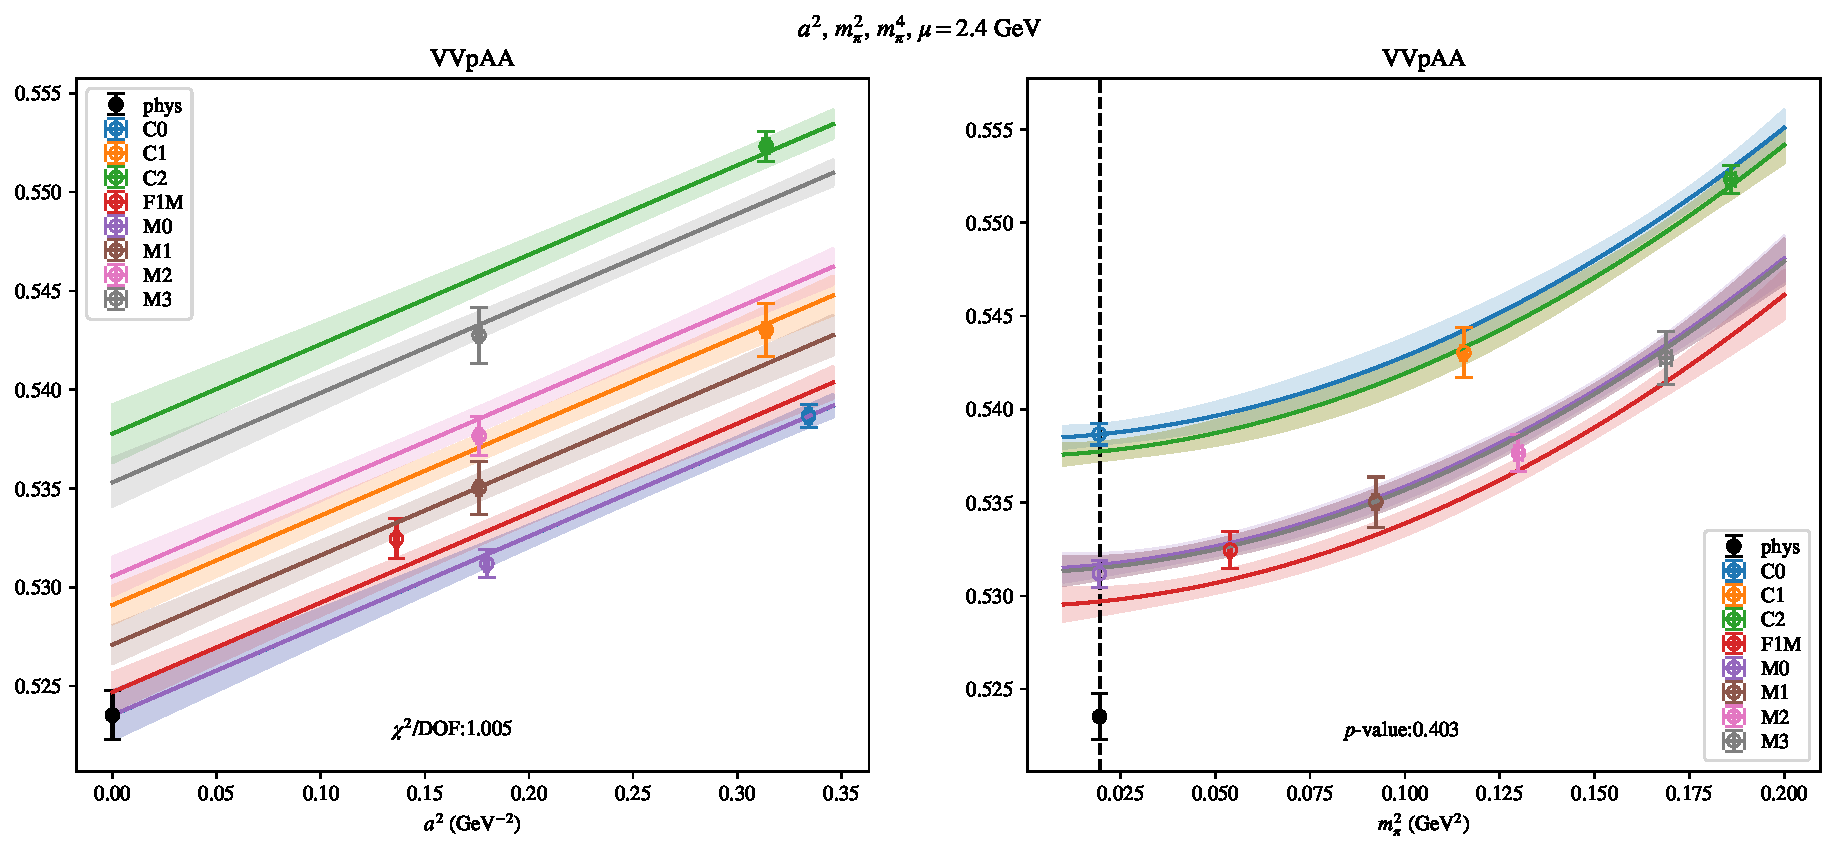
\includepdf[link, pages=-]{VVpAA/NPR/a2m2m4_24.pdf}
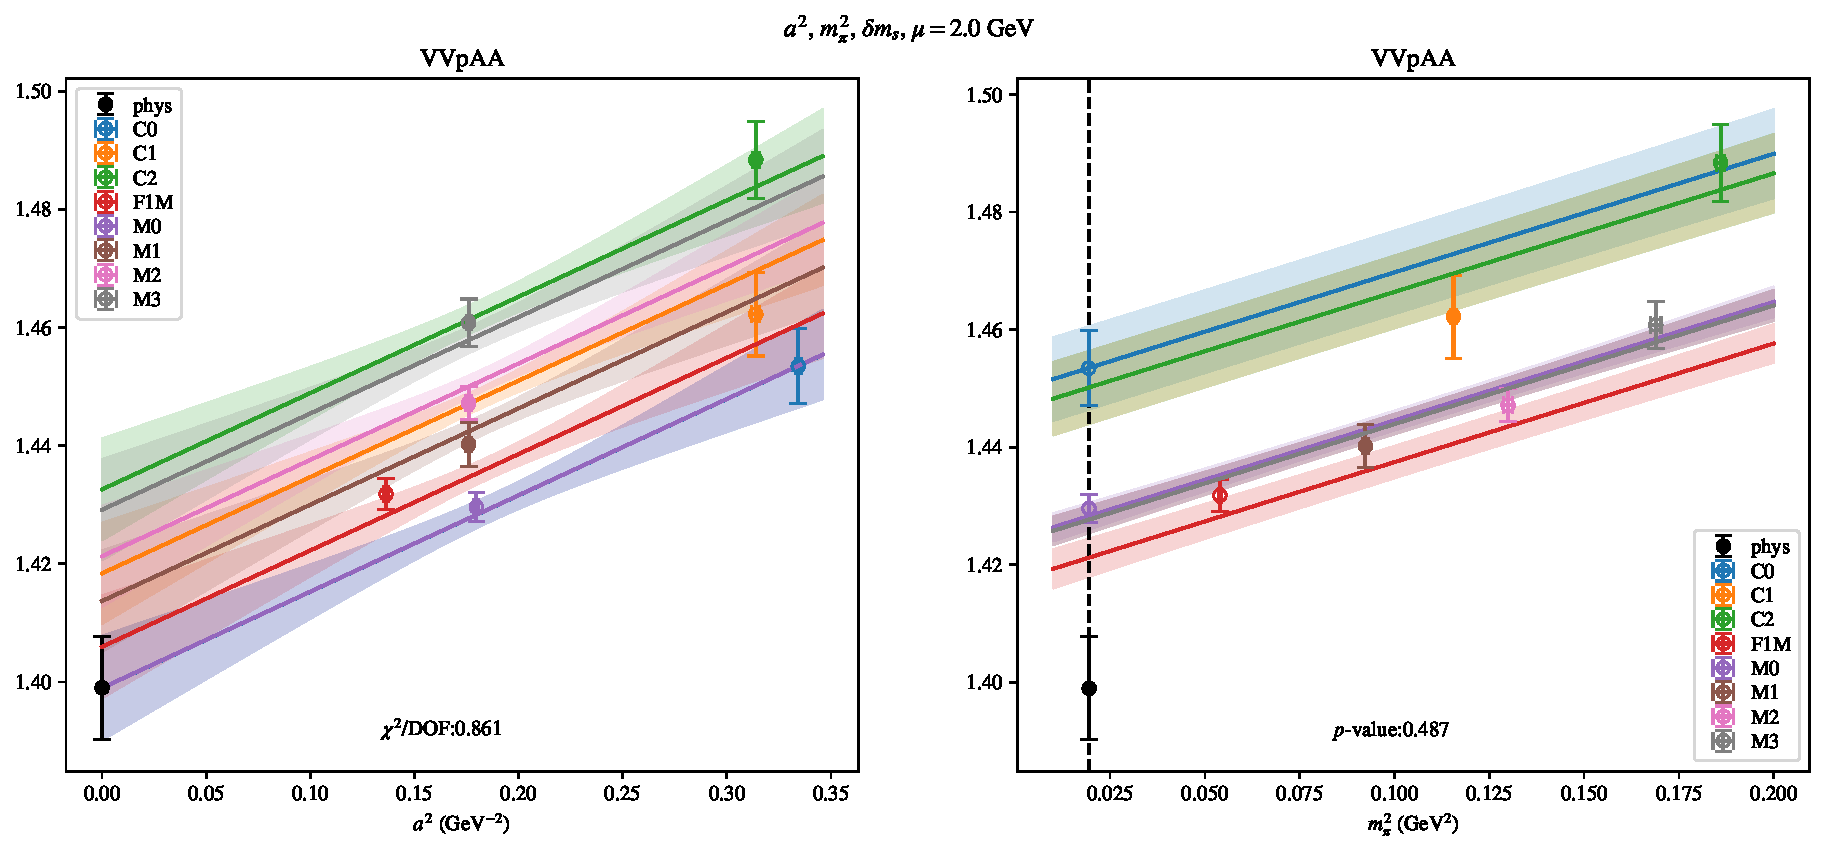
\includepdf[link, pages=-]{VVpAA/NPR/a2m2delm_20.pdf}
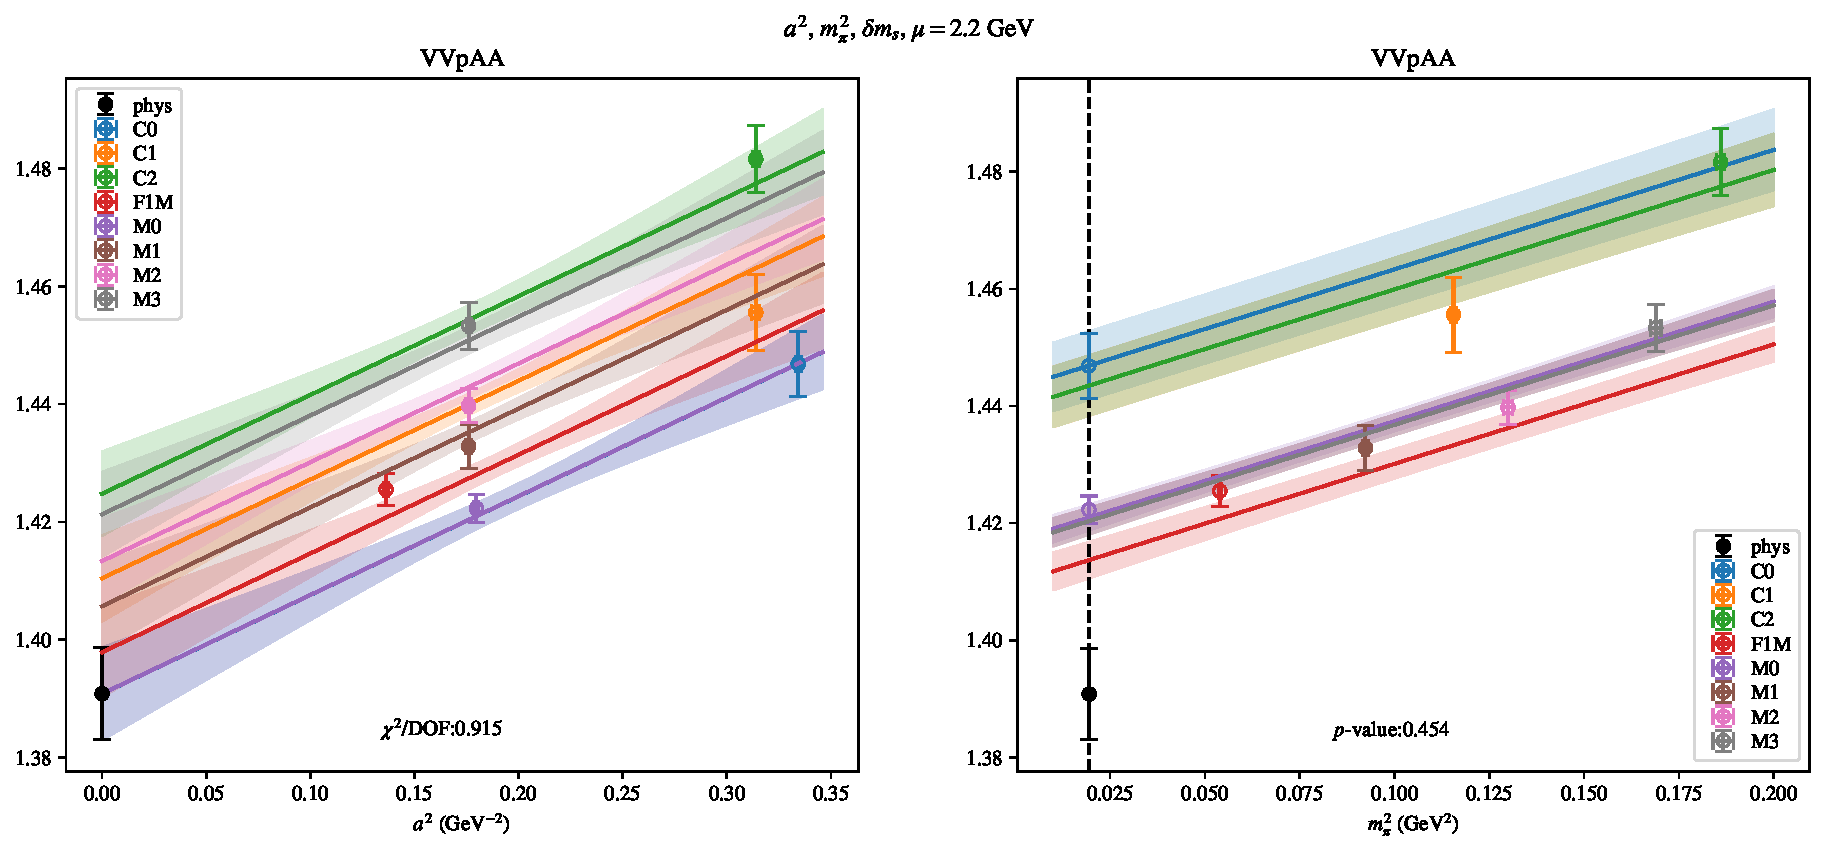
\includepdf[link, pages=-]{VVpAA/NPR/a2m2delm_22.pdf}
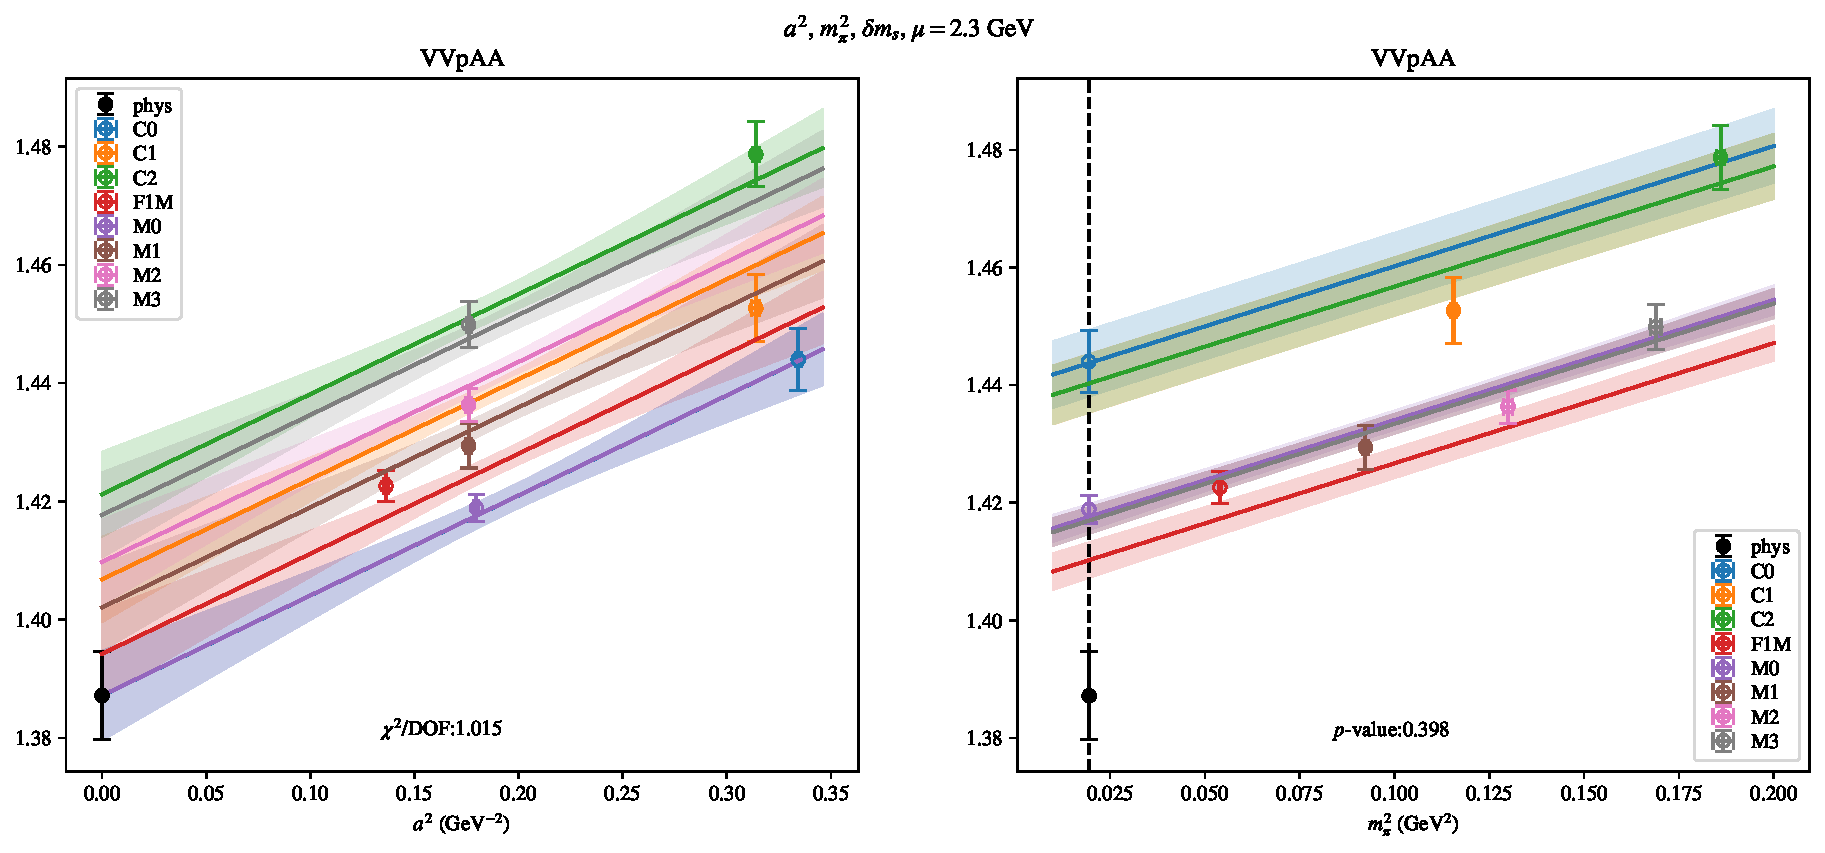
\includepdf[link, pages=-]{VVpAA/NPR/a2m2delm_23.pdf}
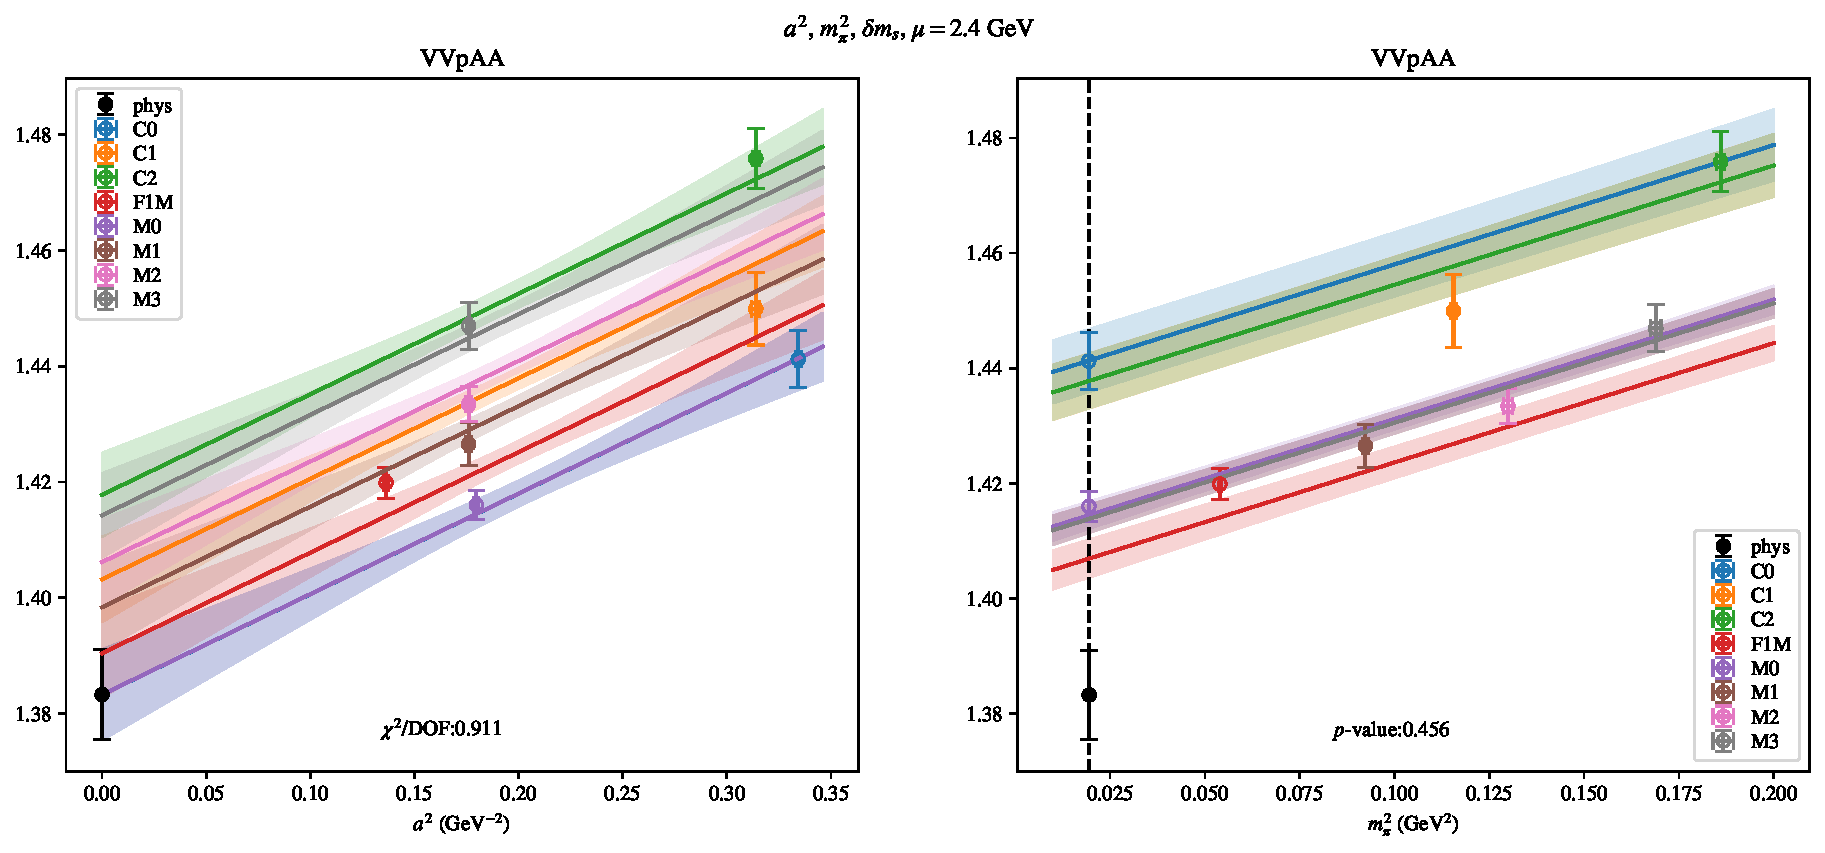
\includepdf[link, pages=-]{VVpAA/NPR/a2m2delm_24.pdf}
\clearpage
\section{$\mathcal{B}_2$}
\begin{table}[h!]
\begin{center}
\begin{tabular}{|c|c|c|c|c|c|c|}
\hline
$\mu$ (GeV) & $a^2$, $m_\pi^2$& $a^2$, $m_\pi^2$ (no C)& $a^2$, $m_\pi^2$, $a^4$& $a^2$, $m_\pi^2$ (no M3, C2)& $a^2$, $m_\pi^2$, $m_\pi^4$& $a^2$, $m_\pi^2$, $\delta m_s$\\
\hline
2.0& \hyperlink{VVmAA/NPR/a2m2_20.pdf.1}{\textbf{-0.94(36)}: 0.048 (0.999)} & \hyperlink{VVmAA/NPR/a2m2noC_20.pdf.1}{\textbf{-0.91(18)}: 0.467 (0.627)} & \hyperlink{VVmAA/NPR/a2a4m2_20.pdf.1}{\textbf{-0.4(53)}: 0.012 (1.0)} & \hyperlink{VVmAA/NPR/a2m2mcut_20.pdf.1}{\textbf{-0.97(31)}: 0.064 (0.979)} & \hyperlink{VVmAA/NPR/a2m2m4_20.pdf.1}{\textbf{-0.91(62)}: 0.063 (0.993)} & \hyperlink{VVmAA/NPR/a2m2delm_20.pdf.1}{\textbf{-1.0(15)}: 0.006 (1.0)}\\
2.2& \hyperlink{VVmAA/NPR/a2m2_22.pdf.1}{\textbf{-0.97(24)}: 0.056 (0.998)} & \hyperlink{VVmAA/NPR/a2m2noC_22.pdf.1}{\textbf{-0.95(14)}: 0.809 (0.445)} & \hyperlink{VVmAA/NPR/a2a4m2_22.pdf.1}{\textbf{-0.5(49)}: 0.013 (1.0)} & \hyperlink{VVmAA/NPR/a2m2mcut_22.pdf.1}{\textbf{-1.00(31)}: 0.062 (0.98)} & \hyperlink{VVmAA/NPR/a2m2m4_22.pdf.1}{\textbf{-0.99(27)}: 0.056 (0.994)} & \hyperlink{VVmAA/NPR/a2m2delm_22.pdf.1}{\textbf{-0.8(17)}: 0.011 (1.0)}\\
2.3& \hyperlink{VVmAA/NPR/a2m2_23.pdf.1}{\textbf{-0.96(29)}: 0.064 (0.997)} & \hyperlink{VVmAA/NPR/a2m2noC_23.pdf.1}{\textbf{-0.96(14)}: 1.161 (0.313)} & \hyperlink{VVmAA/NPR/a2a4m2_23.pdf.1}{\textbf{-1.3(47)}: 0.017 (0.999)} & \hyperlink{VVmAA/NPR/a2m2mcut_23.pdf.1}{\textbf{-1.00(33)}: 0.078 (0.972)} & \hyperlink{VVmAA/NPR/a2m2m4_23.pdf.1}{\textbf{-1.03(48)}: 0.078 (0.989)} & \hyperlink{VVmAA/NPR/a2m2delm_23.pdf.1}{\textbf{-1.02(75)}: 0.013 (1.0)}\\
2.4& \hyperlink{VVmAA/NPR/a2m2_24.pdf.1}{\textbf{-1.01(33)}: 0.085 (0.995)} & \hyperlink{VVmAA/NPR/a2m2noC_24.pdf.1}{\textbf{-0.97(12)}: 1.527 (0.217)} & \hyperlink{VVmAA/NPR/a2a4m2_24.pdf.1}{\textbf{-1.0(22)}: 0.022 (0.999)} & \hyperlink{VVmAA/NPR/a2m2mcut_24.pdf.1}{\textbf{-0.98(26)}: 0.083 (0.969)} & \hyperlink{VVmAA/NPR/a2m2m4_24.pdf.1}{\textbf{-0.98(27)}: 0.087 (0.986)} & \hyperlink{VVmAA/NPR/a2m2delm_24.pdf.1}{\textbf{-0.94(94)}: 0.018 (0.999)}\\
\hline
\end{tabular}
\caption{Physical point value from chiral and continuum extrapolation at renormalisation scale $\mu$. Entries are \textbf{value(error)}: $\chi^2/\text{DOF}$ ($p$-value).}
\end{center}
\end{table}
\begin{table}[h!]
\begin{center}
\begin{tabular}{|c c|c|c|c|c|c|c|}
\hline
$\mu$ (GeV) &  & $a^2$, $m_\pi^2$& $a^2$, $m_\pi^2$ (no C)& $a^2$, $m_\pi^2$, $a^4$& $a^2$, $m_\pi^2$ (no M3, C2)& $a^2$, $m_\pi^2$, $m_\pi^4$& $a^2$, $m_\pi^2$, $\delta m_s$\\
\hline
\multirow{3}{0.5in}{2.0} & $\alpha$ & 0.02& 0.33(14)& 11(24)& -0.1(21)& 0.33(48)& -0.4(52)\\
 & $\beta$ & 0.0065(49)& 0.00204(36)& 0.001& 0.0& 0.0028(28)& -0.0\\
 & $\gamma$ &  &  & -2(53)&  & -0.0003(70)& 0.070(90)\\
\hline
\multirow{3}{0.5in}{2.2} & $\alpha$ & -0.1(16)& 0.045(96)& 9.3(95)& -0.2(19)& -0.1(19)& 0.41(69)\\
 & $\beta$ & 0.0058(43)& 0.00161(38)& -0.0& -0.001(43)& 0.001& 0.0043(32)\\
 & $\gamma$ &  &  & -2(21)&  & -0.0001(50)& -0.07(99)\\
\hline
\multirow{3}{0.5in}{2.3} & $\alpha$ & -0.031& 0.004& -2.(52)& -0.3(23)& -0.4(32)& -0.2(27)\\
 & $\beta$ & 0.0037(27)& 0.00150(38)& 0.00186(66)& 0.0024(28)& -0.002(22)& 0.001\\
 & $\gamma$ &  &  & 5.831&  & 0.00054(43)& 0.021(39)\\
\hline
\multirow{3}{0.5in}{2.4} & $\alpha$ & -0.4(27)& -0.01(83)& -0.52& -0.059& -0.1(18)& 0.12(44)\\
 & $\beta$ & 0.0062(44)& 0.00142(35)& 0.00126(45)& -0.001(50)& 0.001& 0.0019(12)\\
 & $\gamma$ &  &  & 0.481&  & -0.0& -0.004\\
\hline
\end{tabular}
\caption{Fit values of coefficients in $Q = Q_{phys} + \mathbf{\alpha} a^2 + \mathbf{\beta}\left(\frac{m_\pi^2}{f_\pi^2}-\frac{m_{\pi,PDG}^2}{f_\pi^2}\right) + \gamma(\ldots)$}
\end{center}
\end{table}
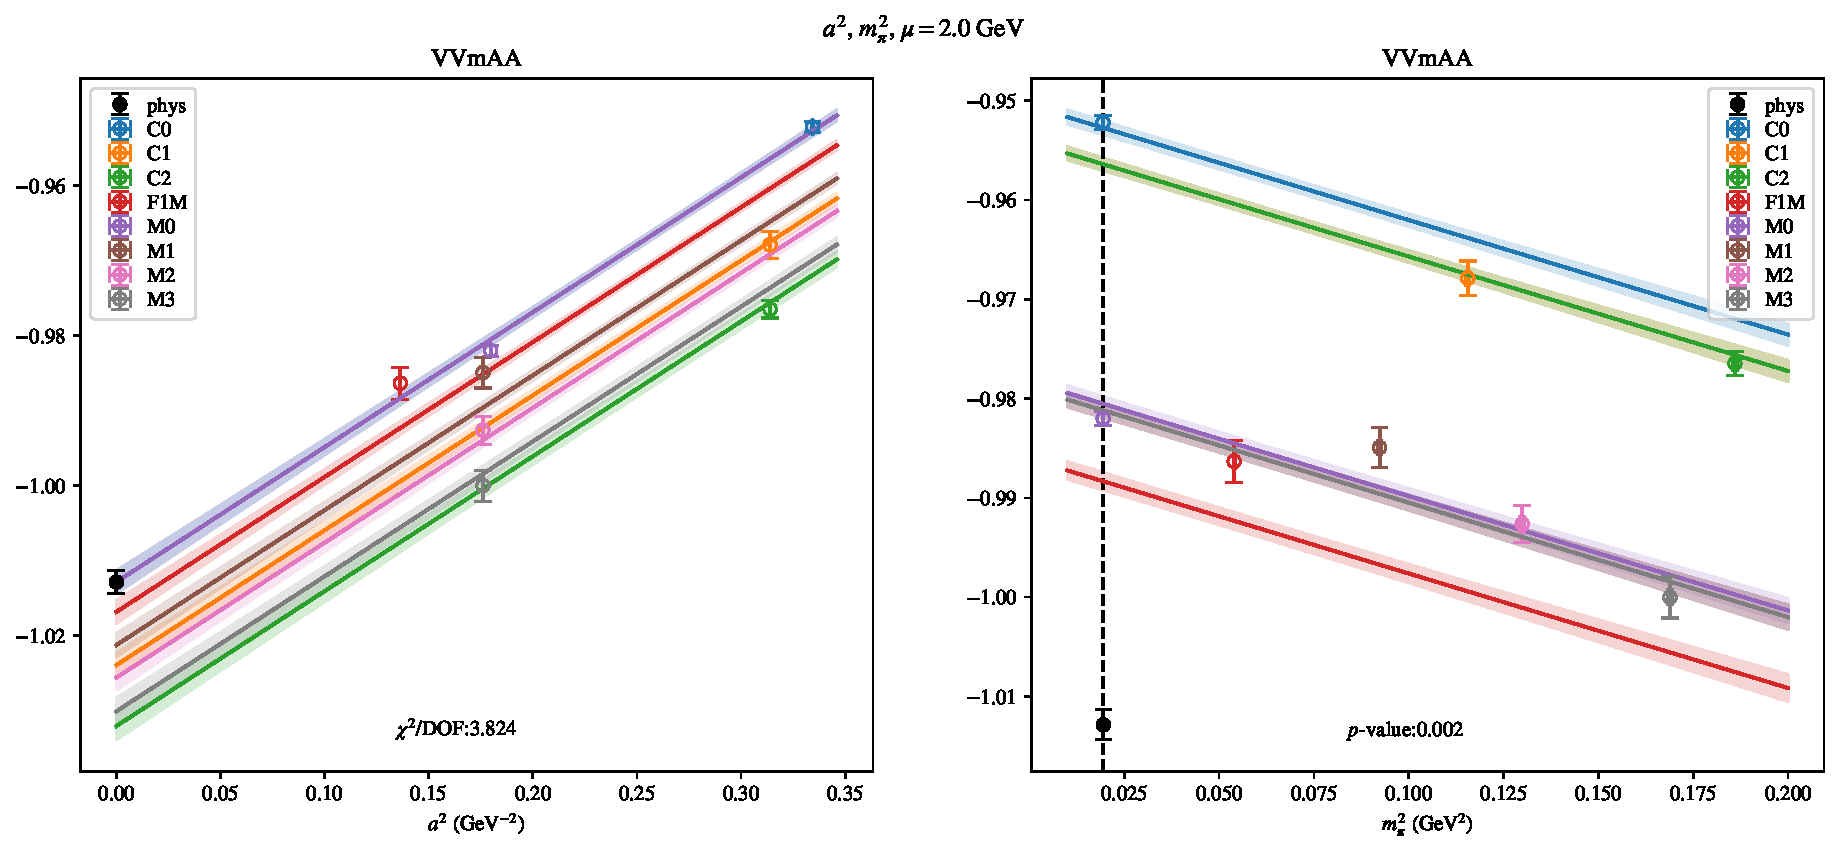
\includepdf[link, pages=-]{VVmAA/NPR/a2m2_20.pdf}
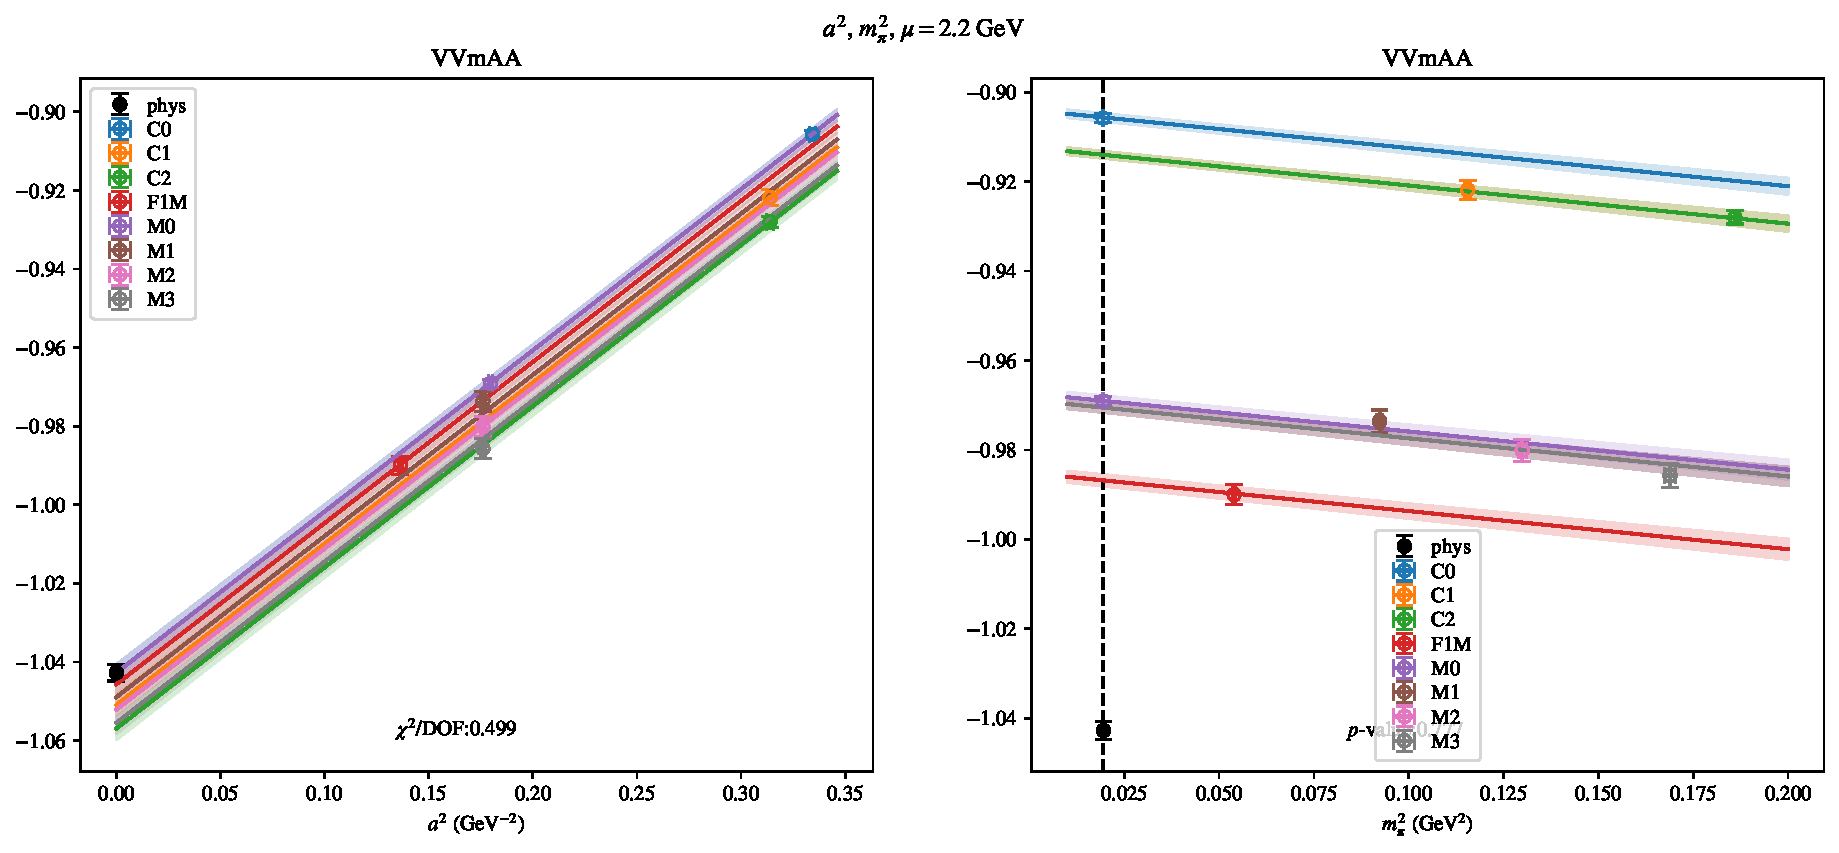
\includepdf[link, pages=-]{VVmAA/NPR/a2m2_22.pdf}
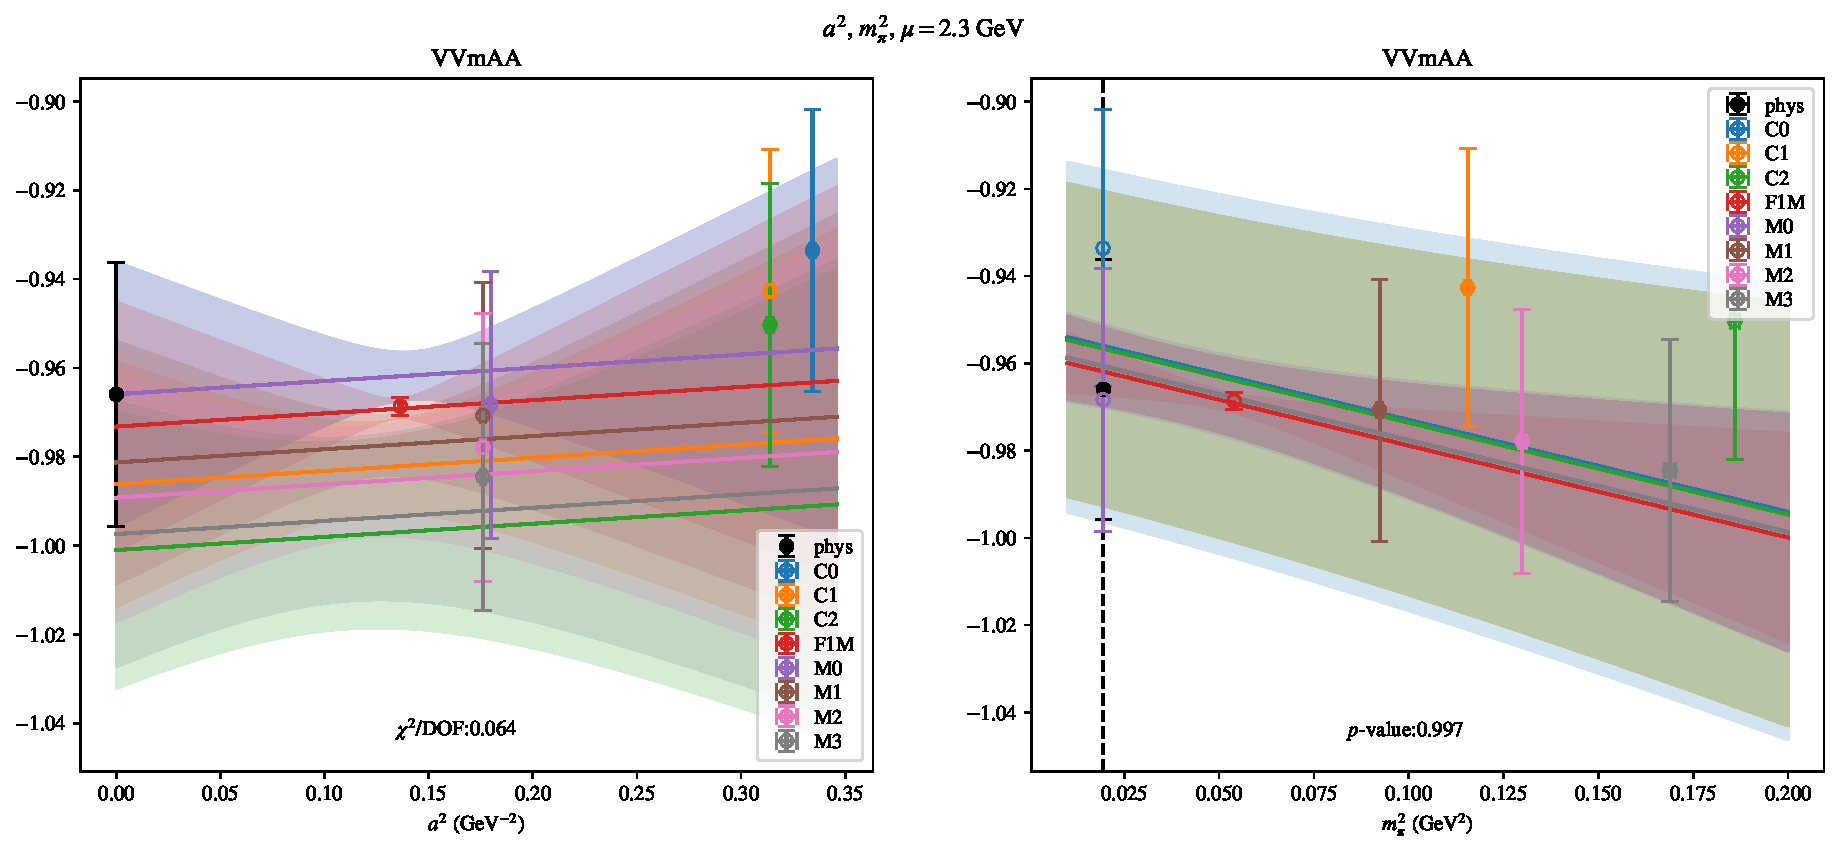
\includepdf[link, pages=-]{VVmAA/NPR/a2m2_23.pdf}
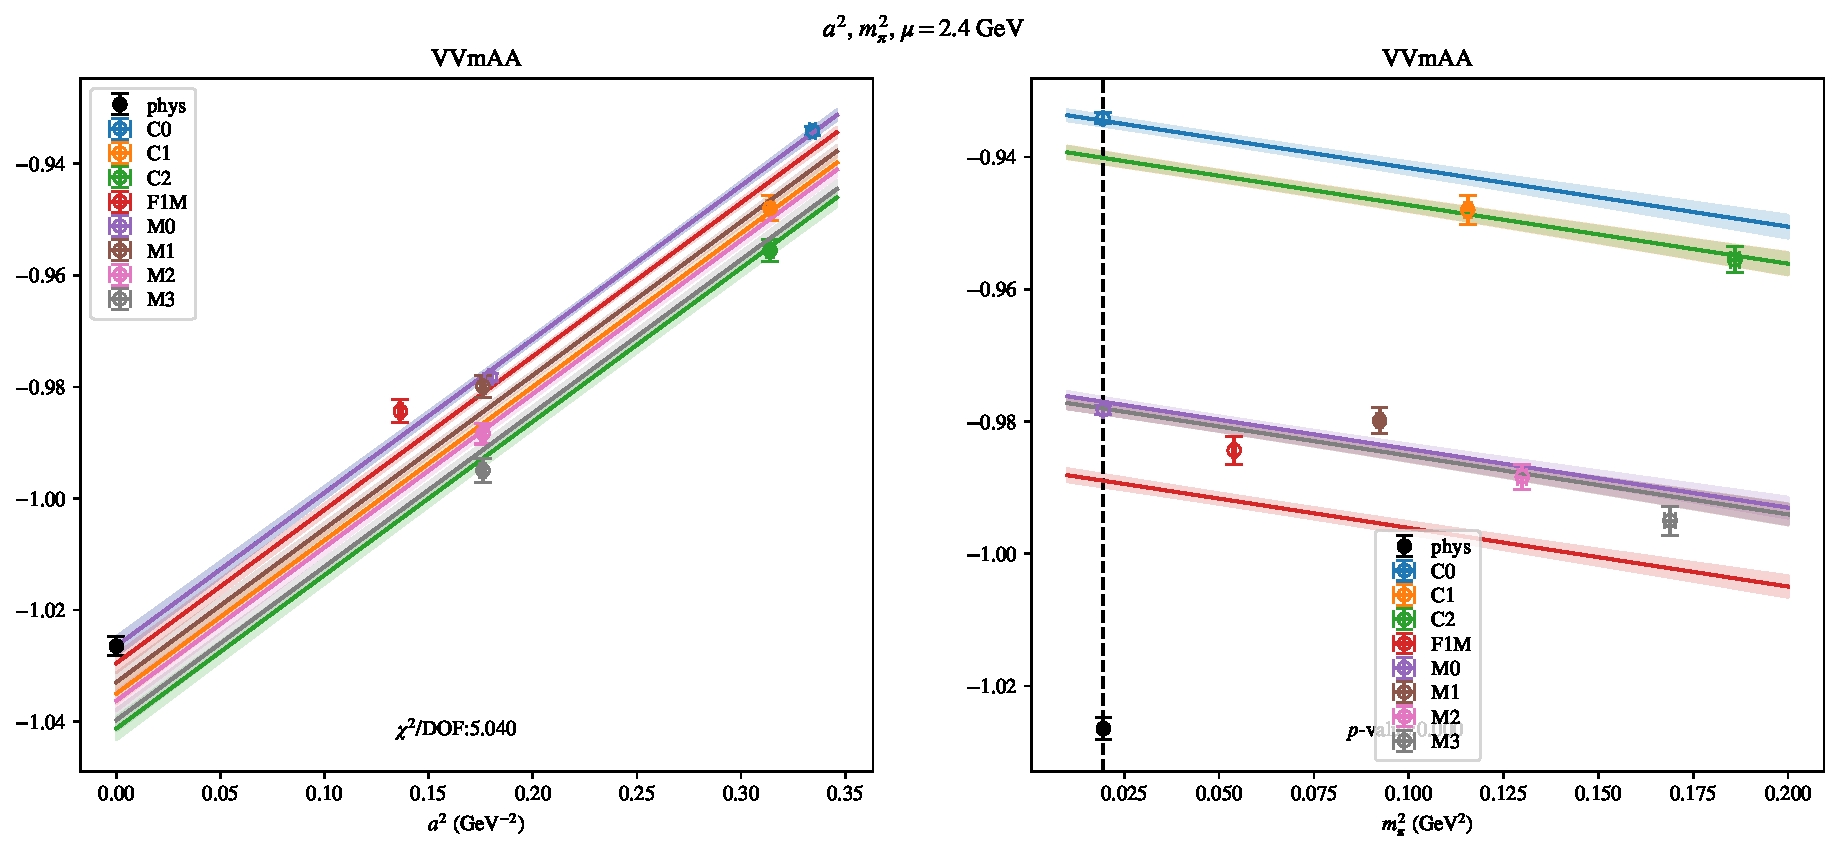
\includepdf[link, pages=-]{VVmAA/NPR/a2m2_24.pdf}
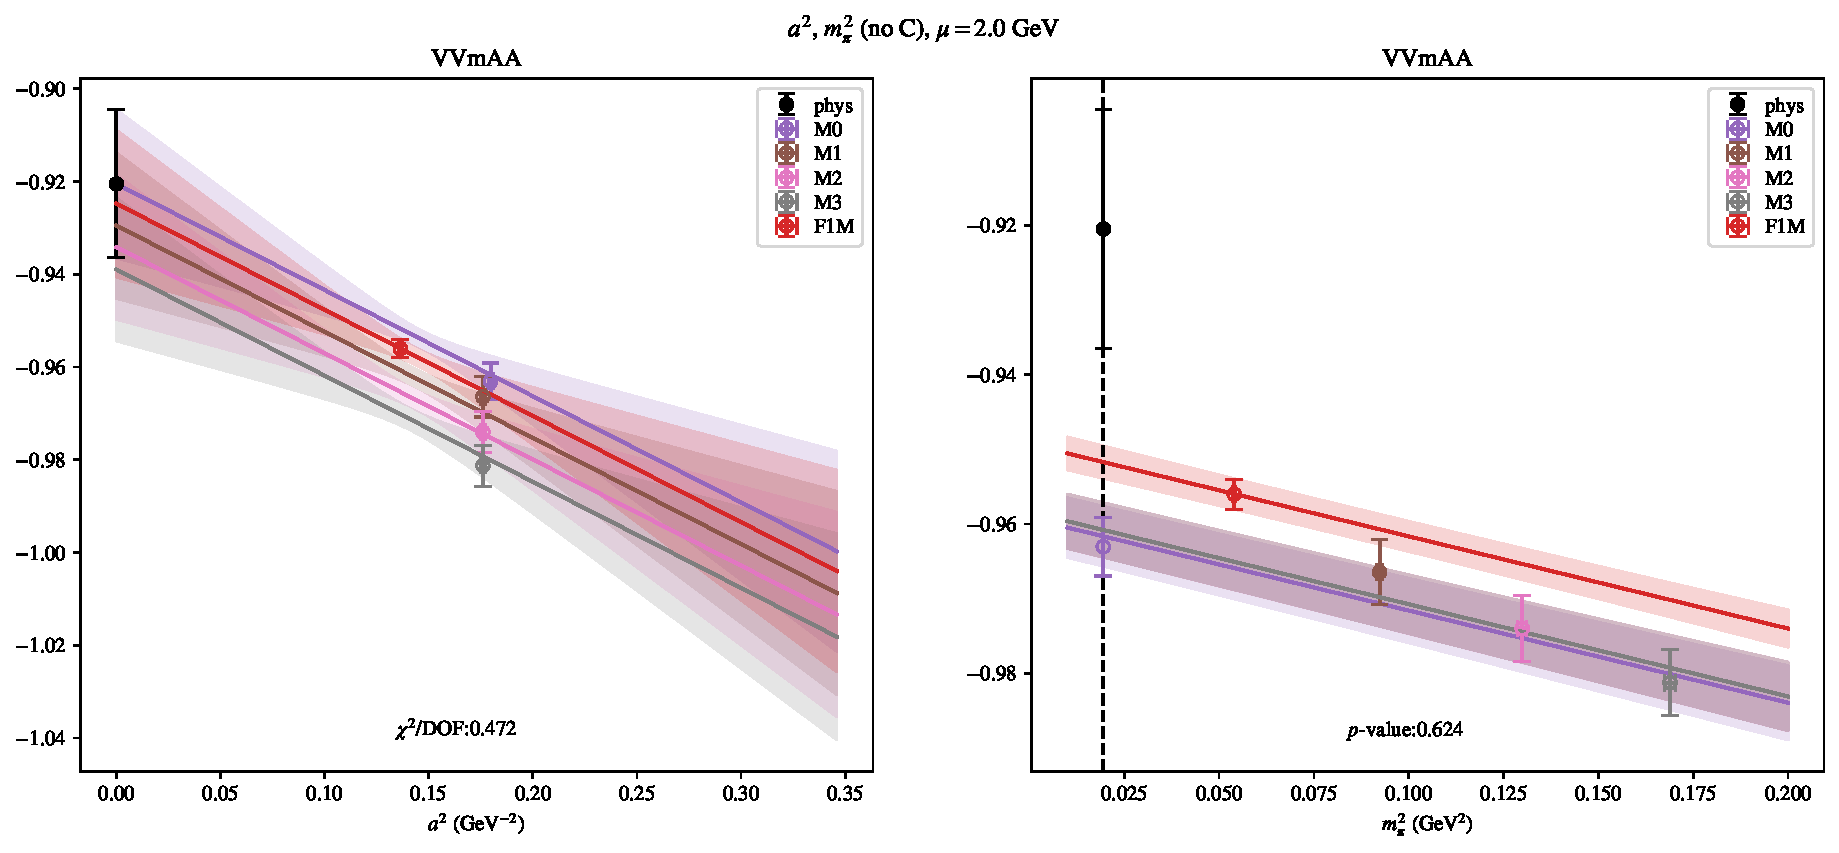
\includepdf[link, pages=-]{VVmAA/NPR/a2m2noC_20.pdf}
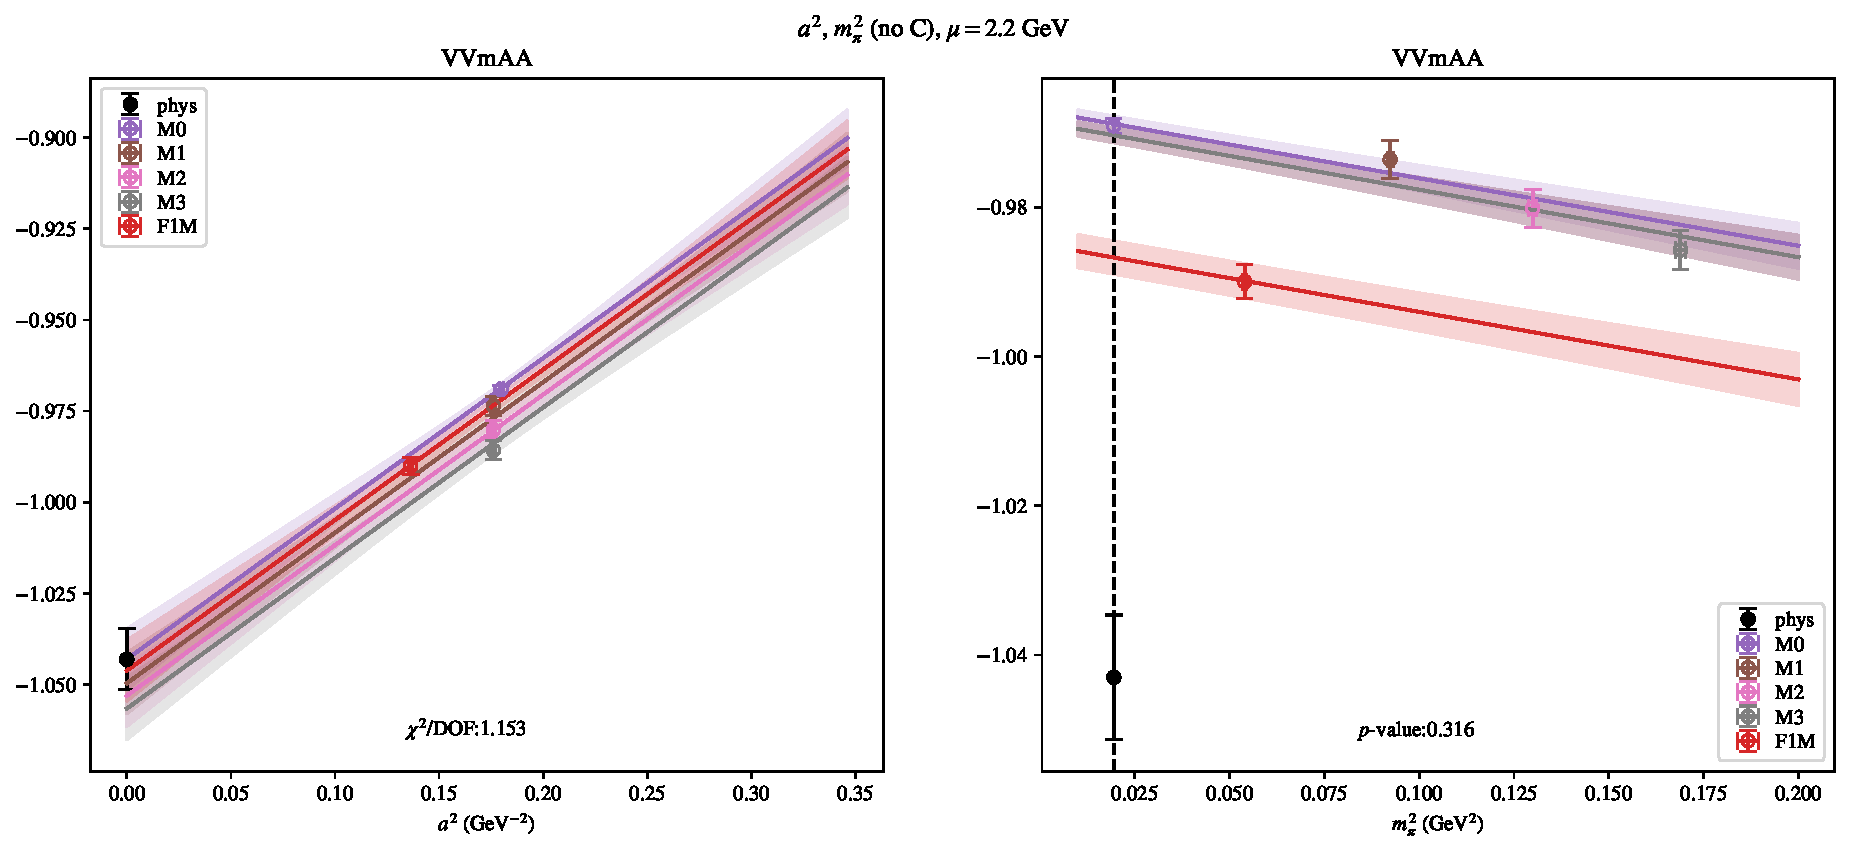
\includepdf[link, pages=-]{VVmAA/NPR/a2m2noC_22.pdf}
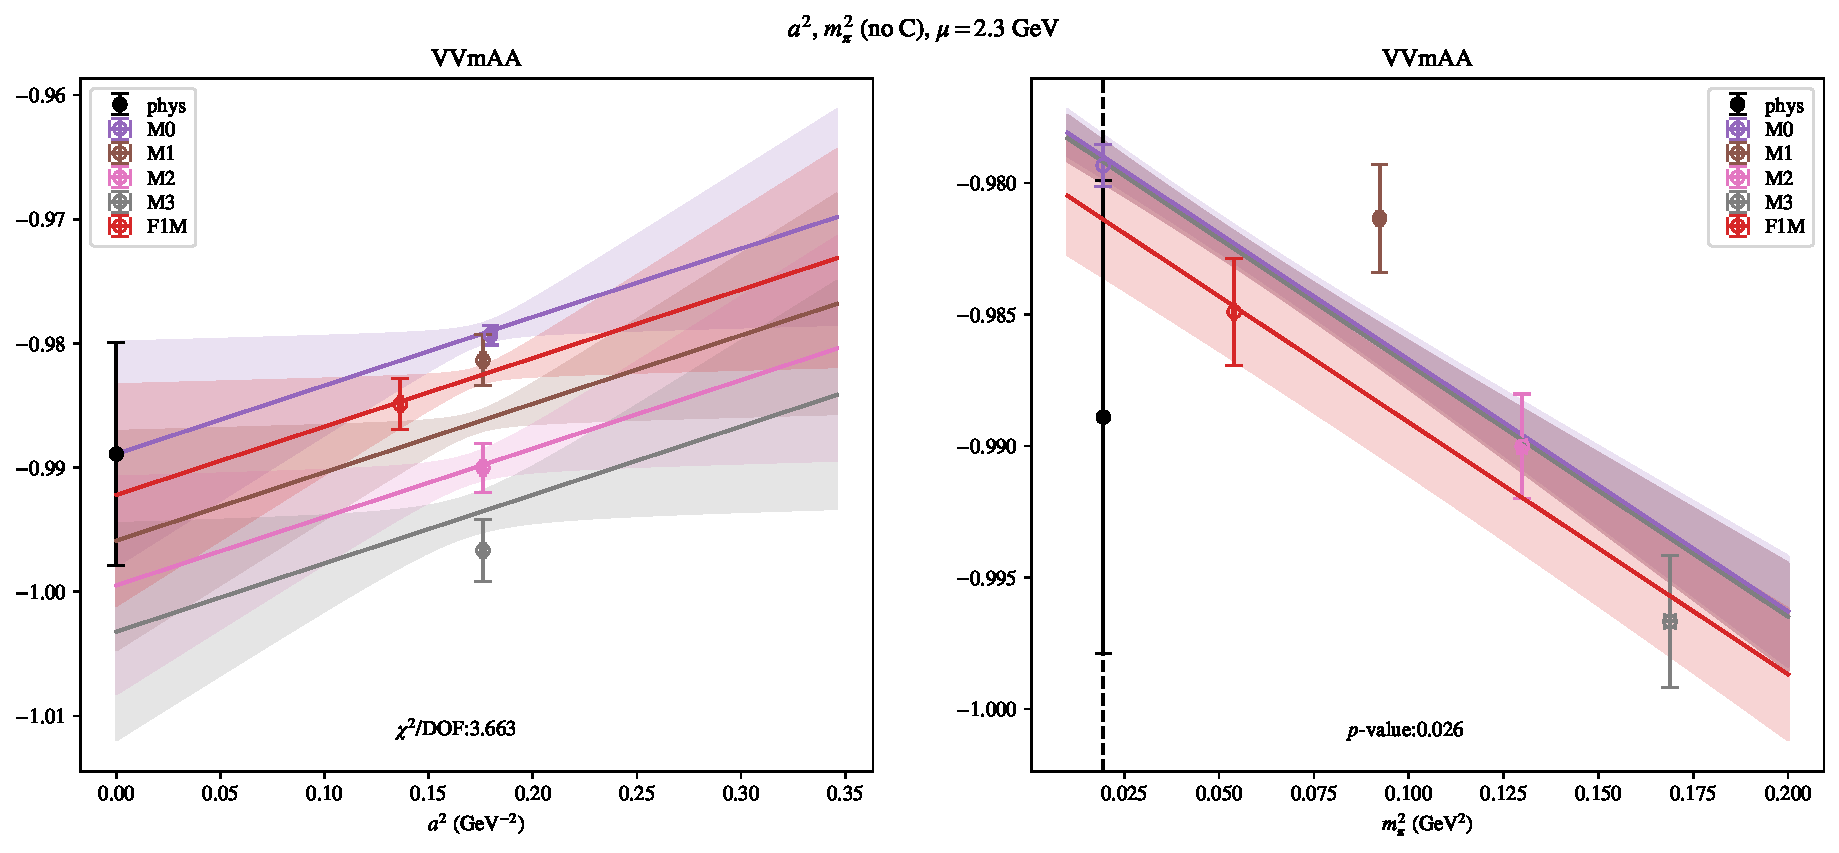
\includepdf[link, pages=-]{VVmAA/NPR/a2m2noC_23.pdf}
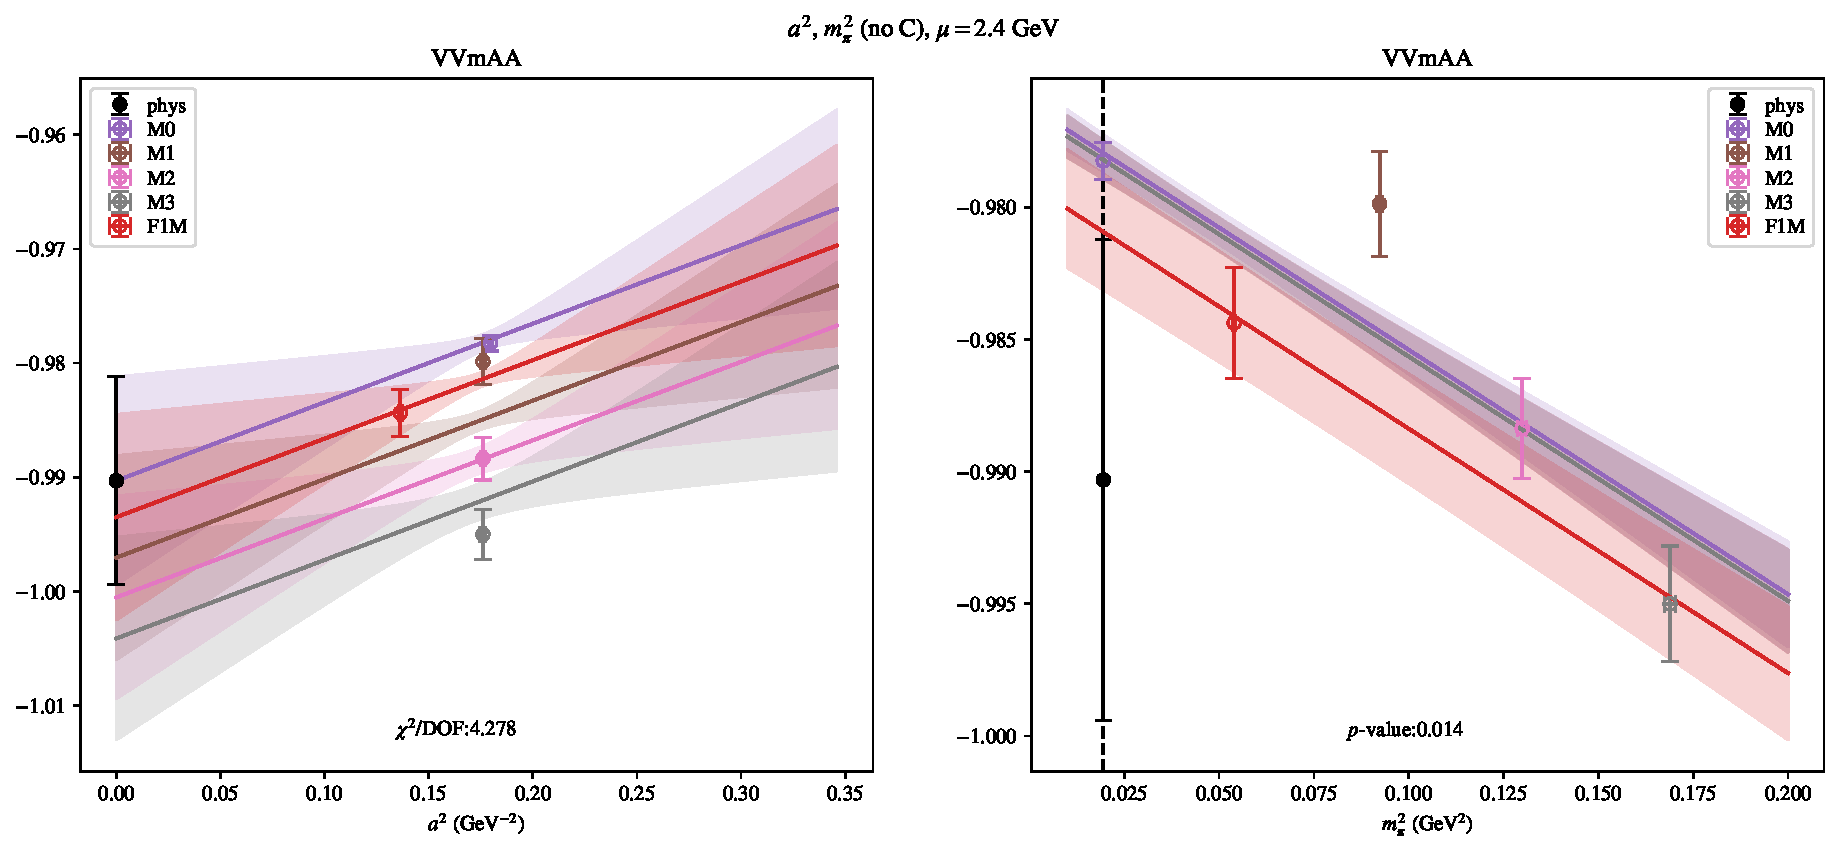
\includepdf[link, pages=-]{VVmAA/NPR/a2m2noC_24.pdf}
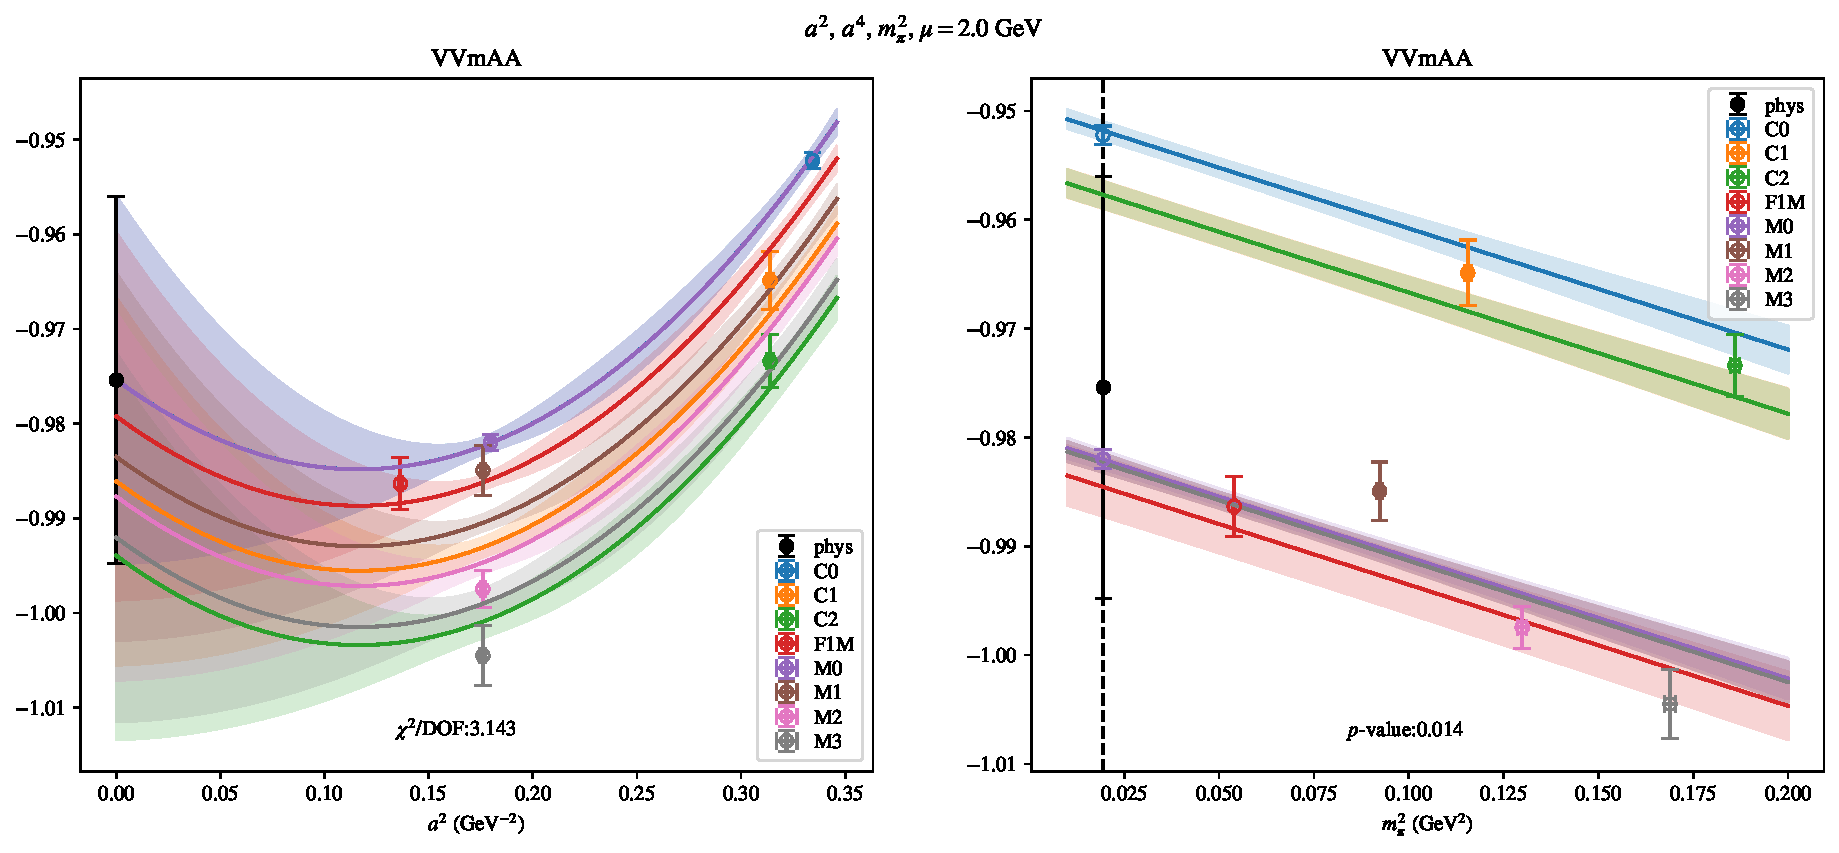
\includepdf[link, pages=-]{VVmAA/NPR/a2a4m2_20.pdf}
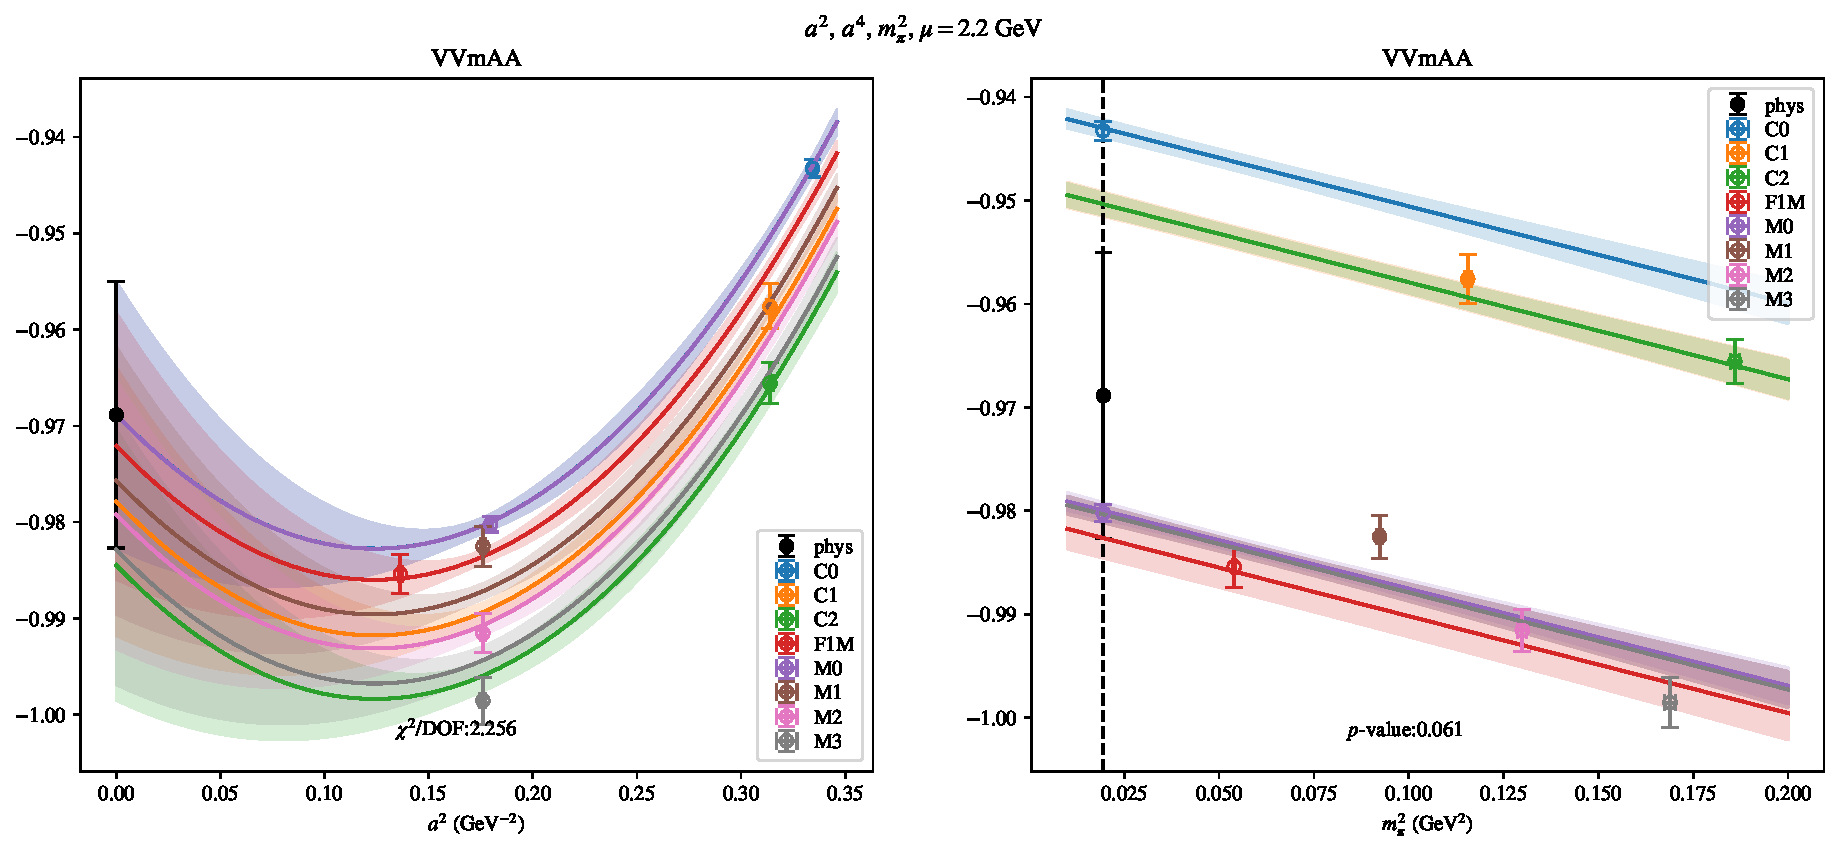
\includepdf[link, pages=-]{VVmAA/NPR/a2a4m2_22.pdf}
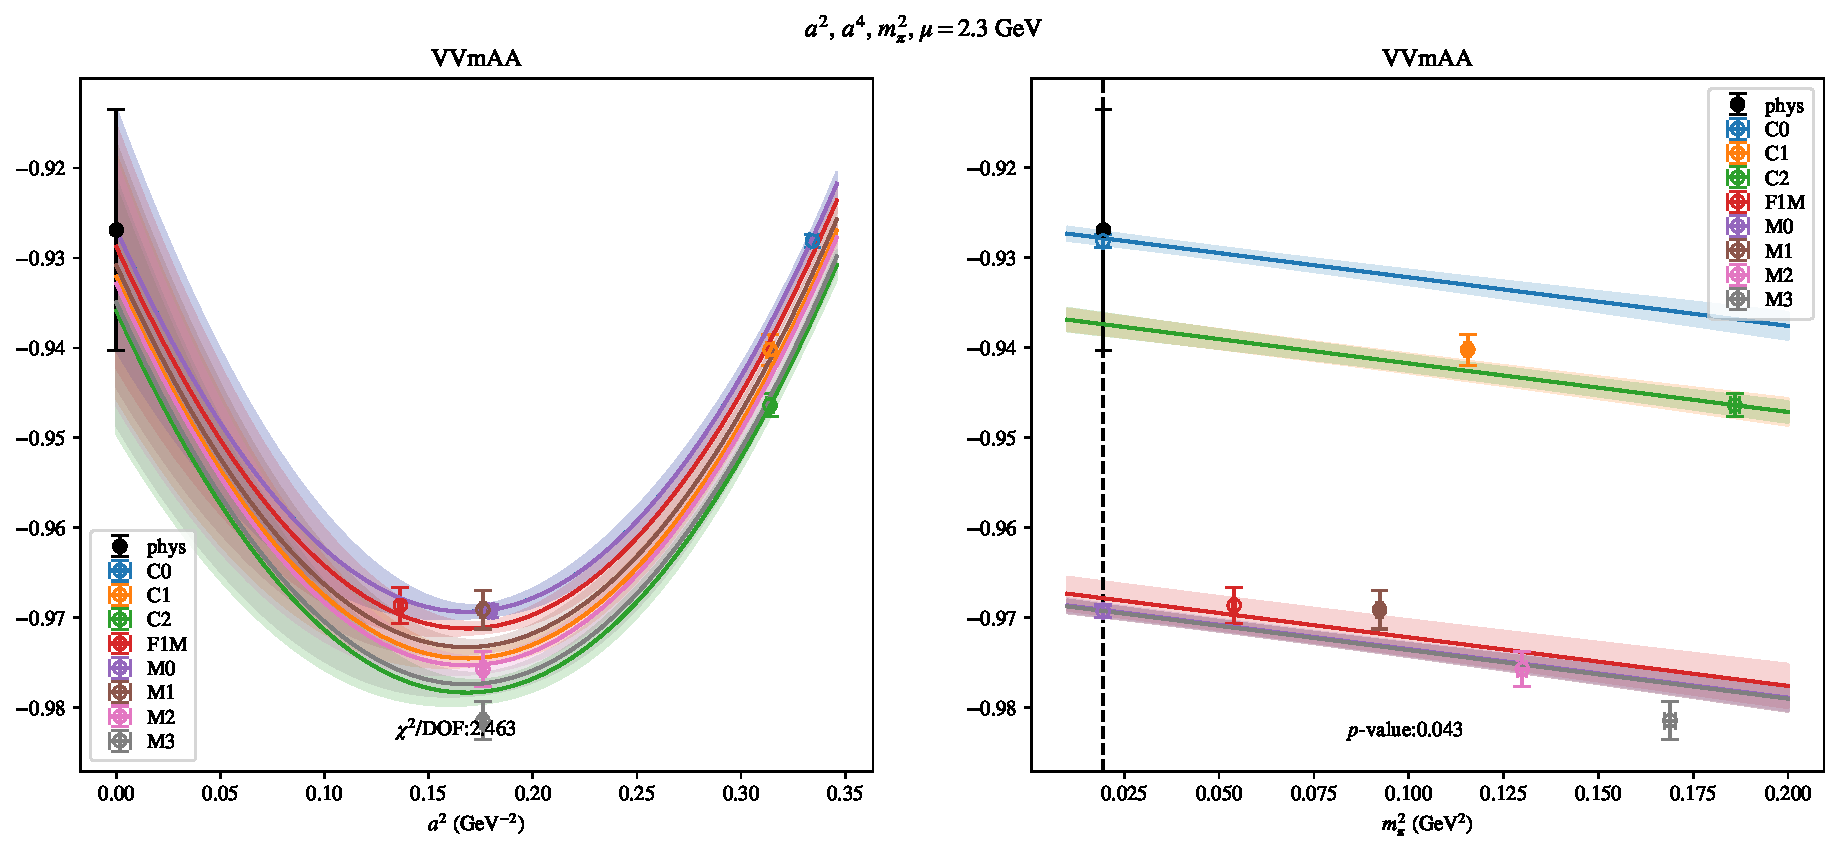
\includepdf[link, pages=-]{VVmAA/NPR/a2a4m2_23.pdf}
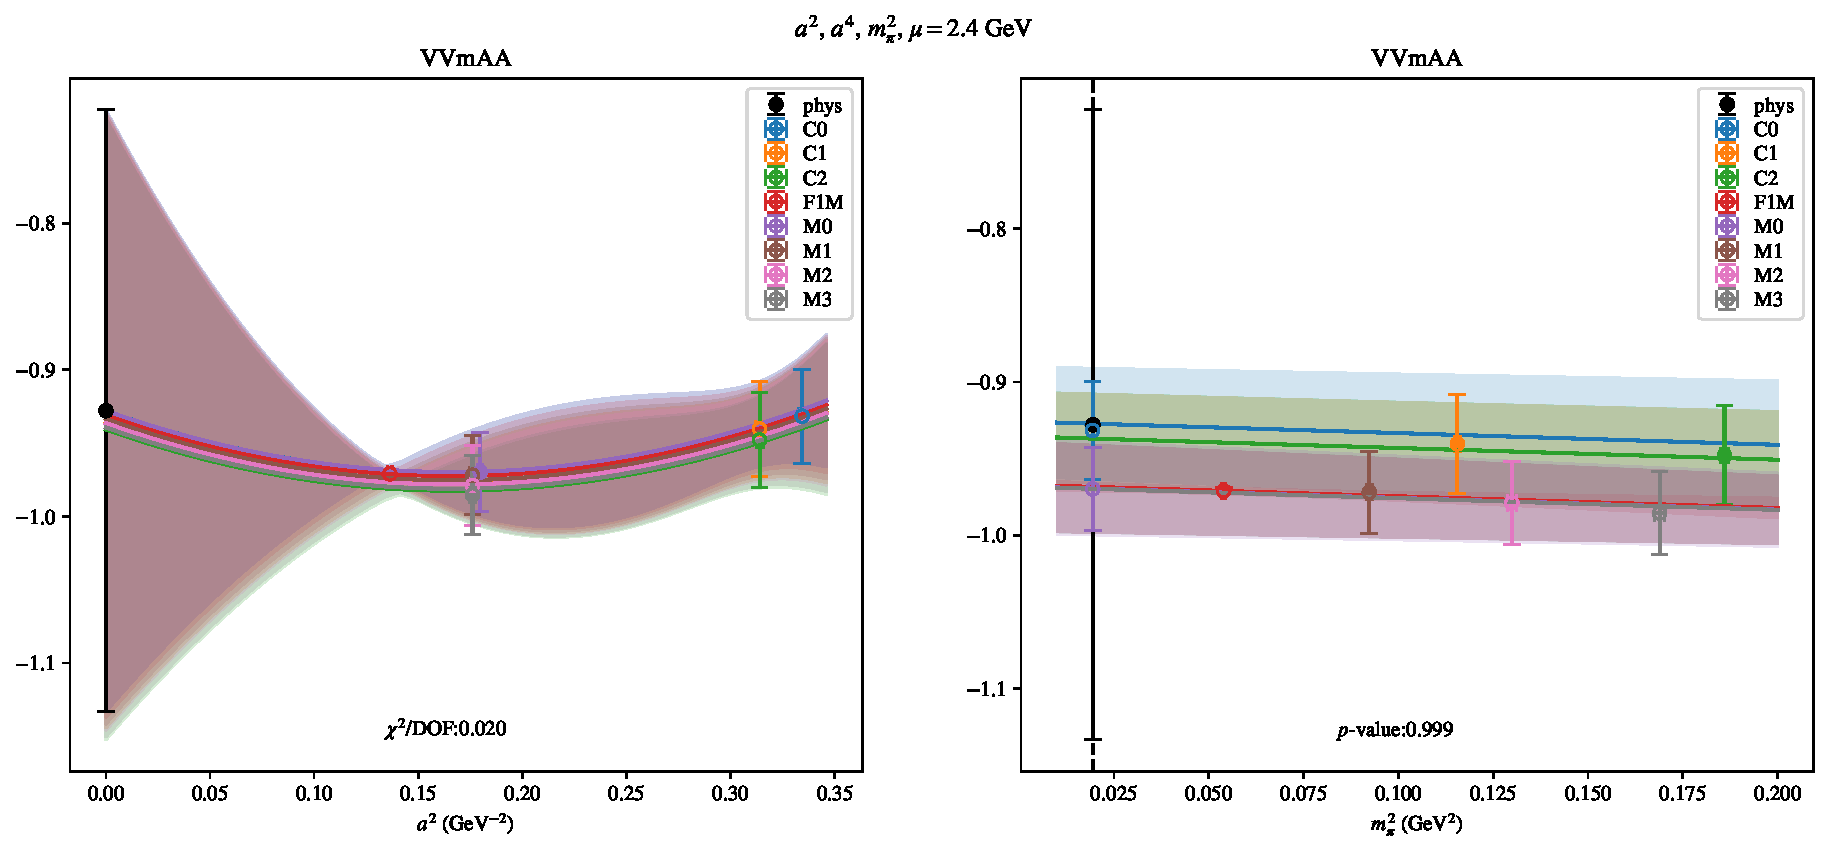
\includepdf[link, pages=-]{VVmAA/NPR/a2a4m2_24.pdf}
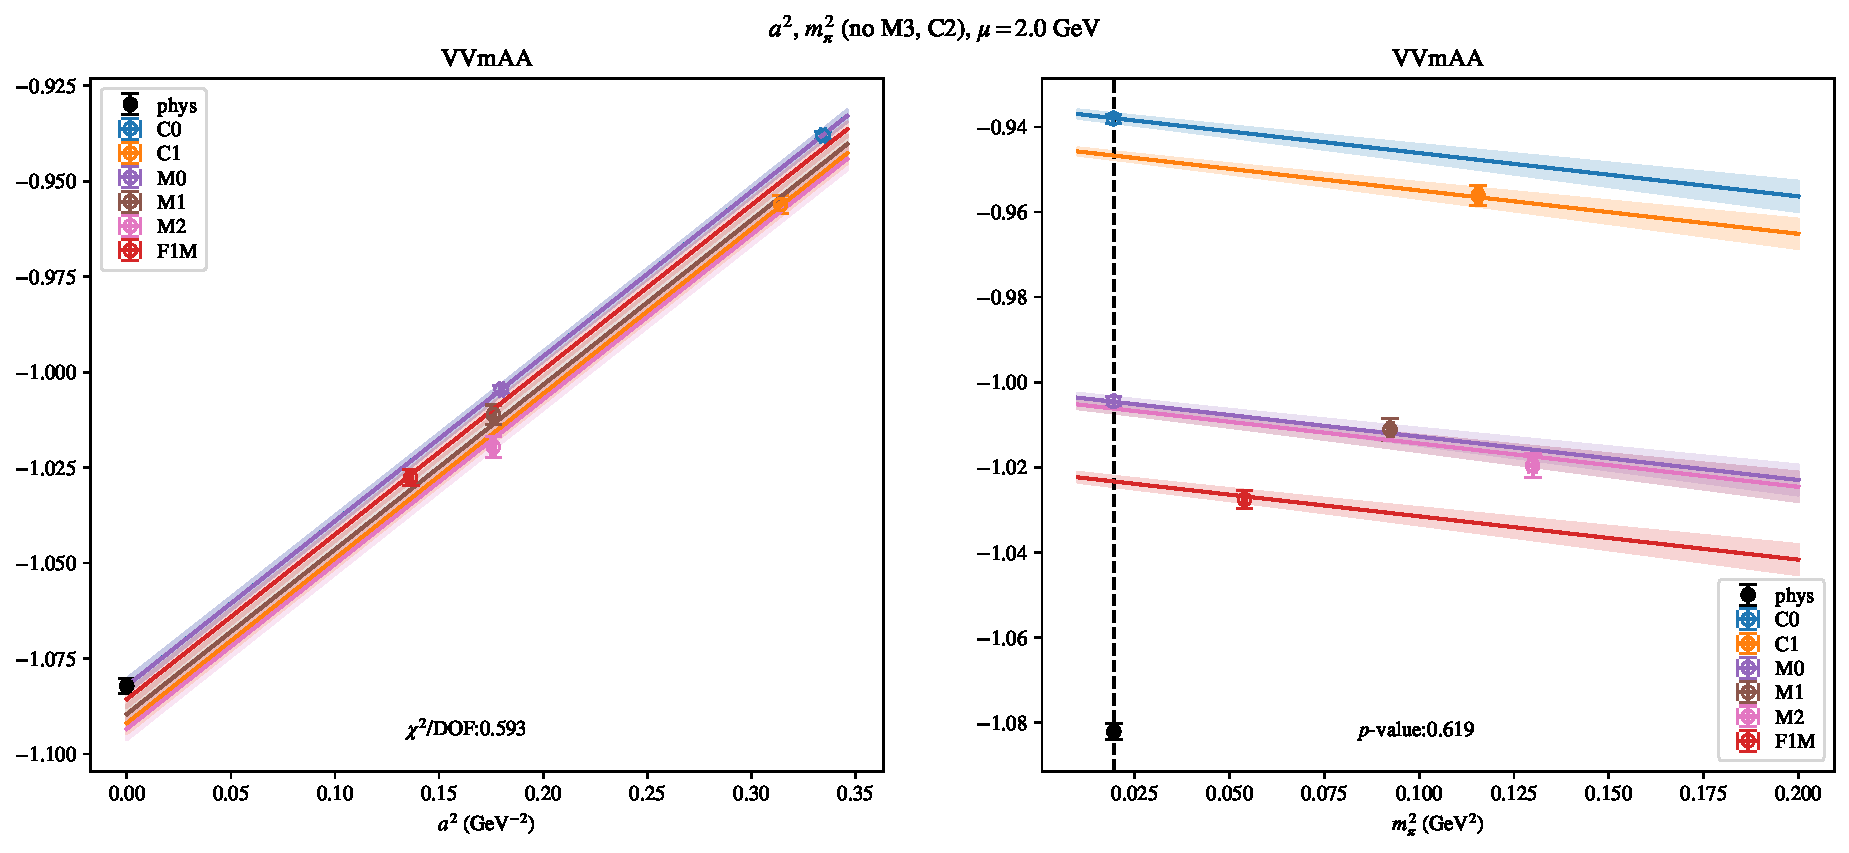
\includepdf[link, pages=-]{VVmAA/NPR/a2m2mcut_20.pdf}
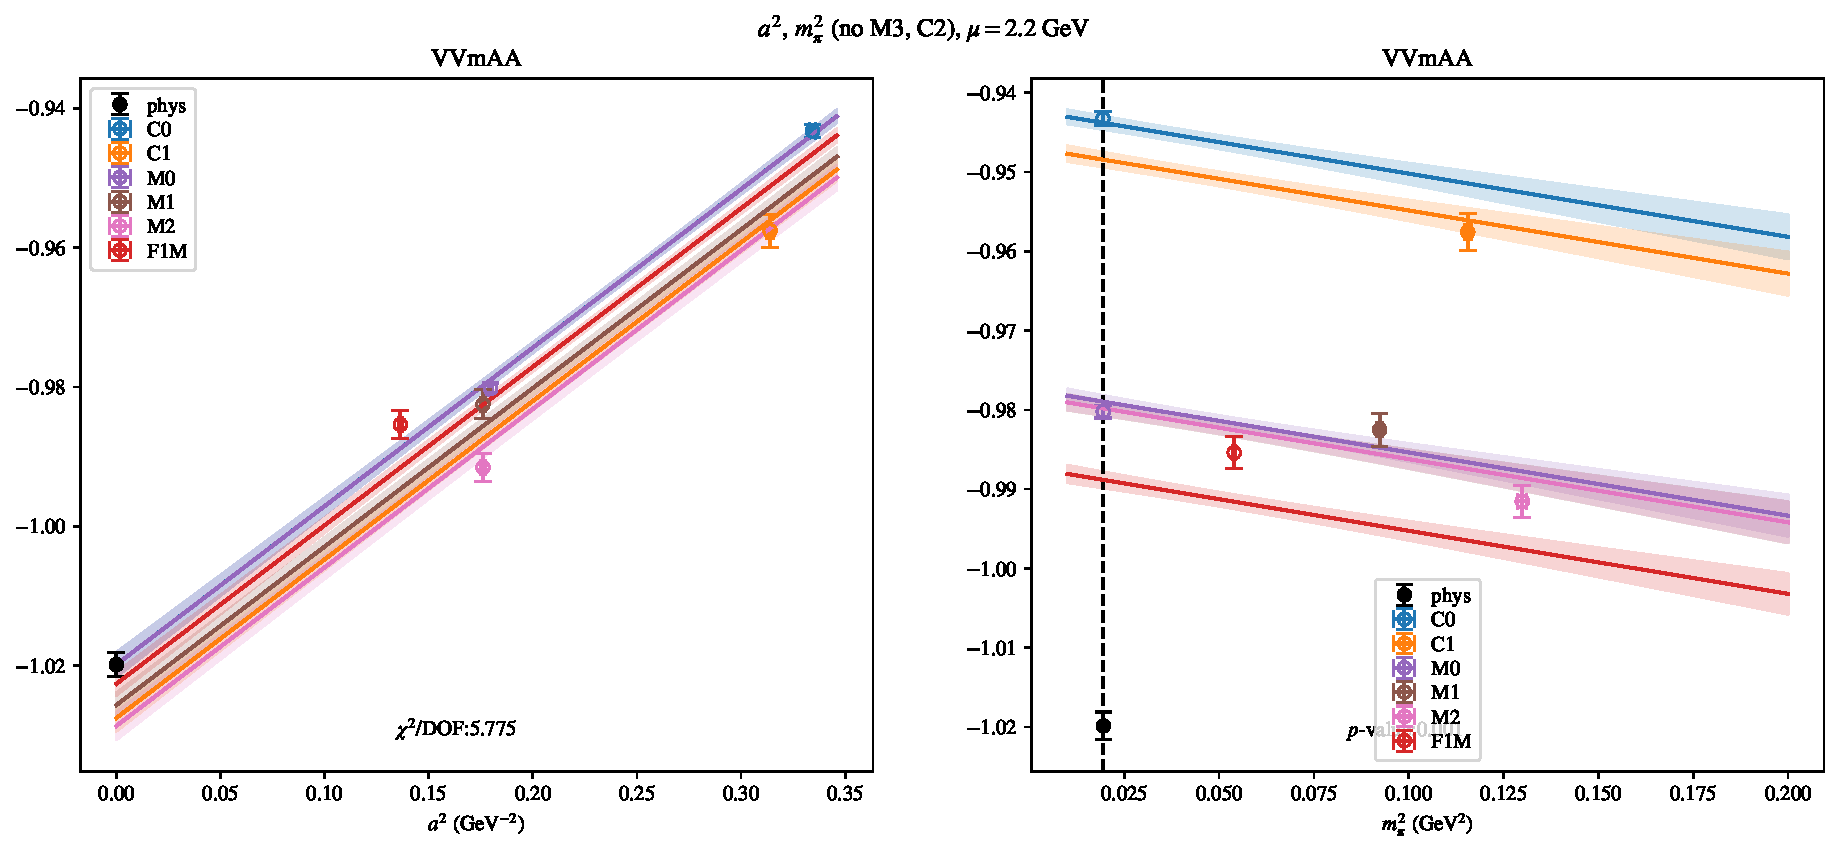
\includepdf[link, pages=-]{VVmAA/NPR/a2m2mcut_22.pdf}
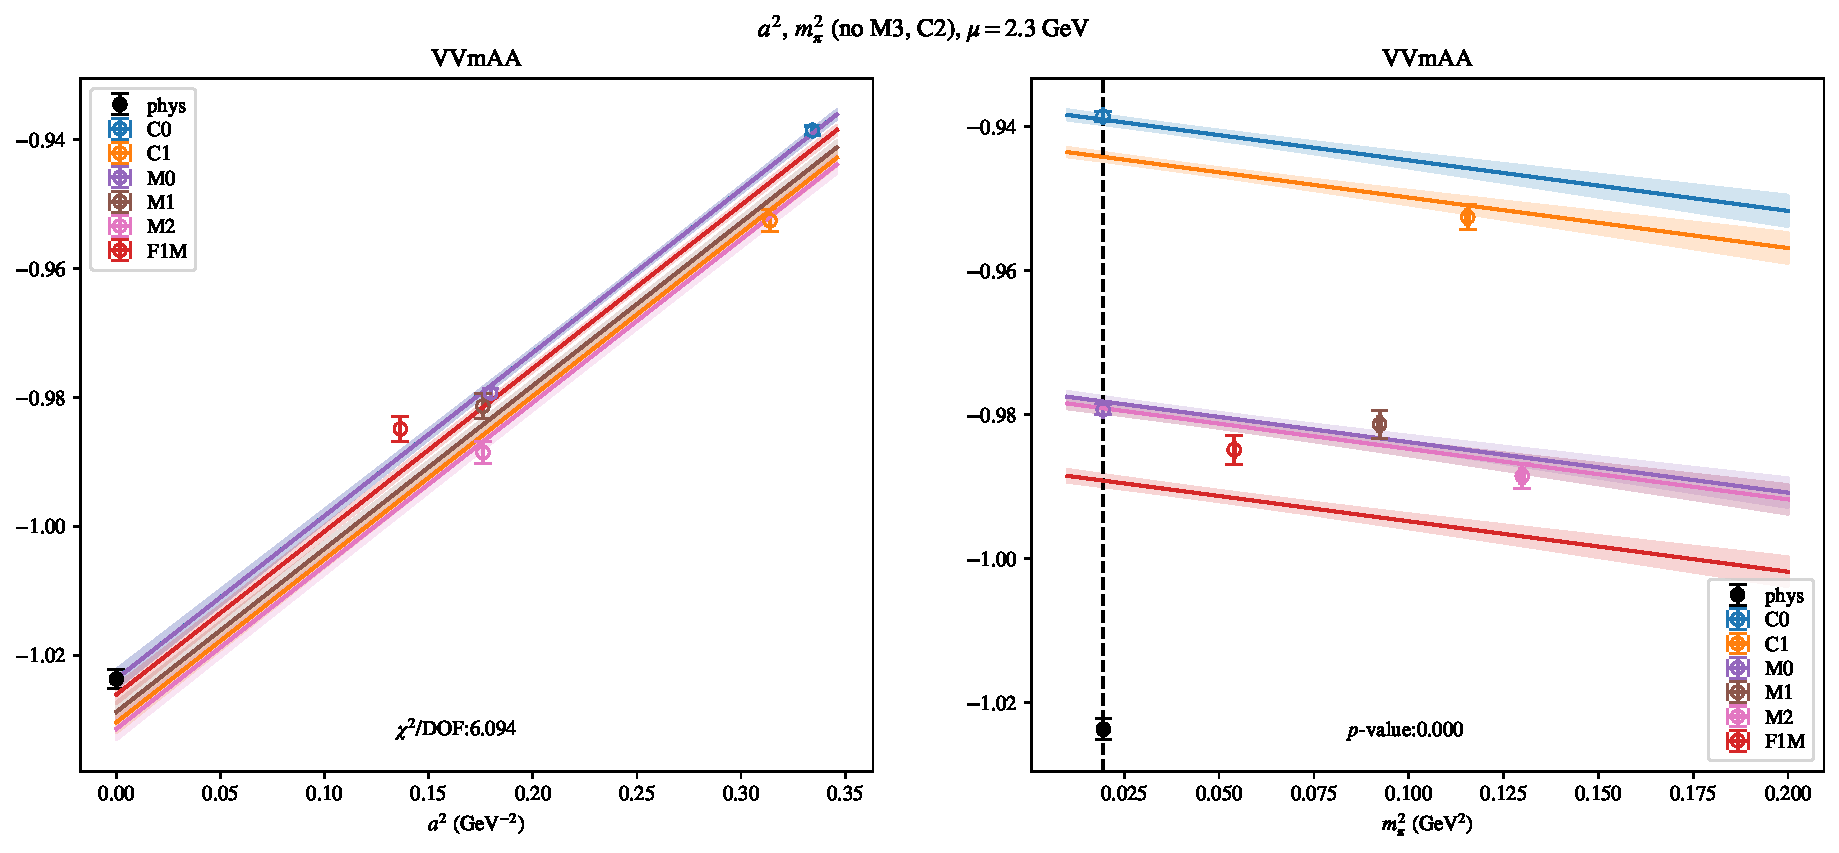
\includepdf[link, pages=-]{VVmAA/NPR/a2m2mcut_23.pdf}
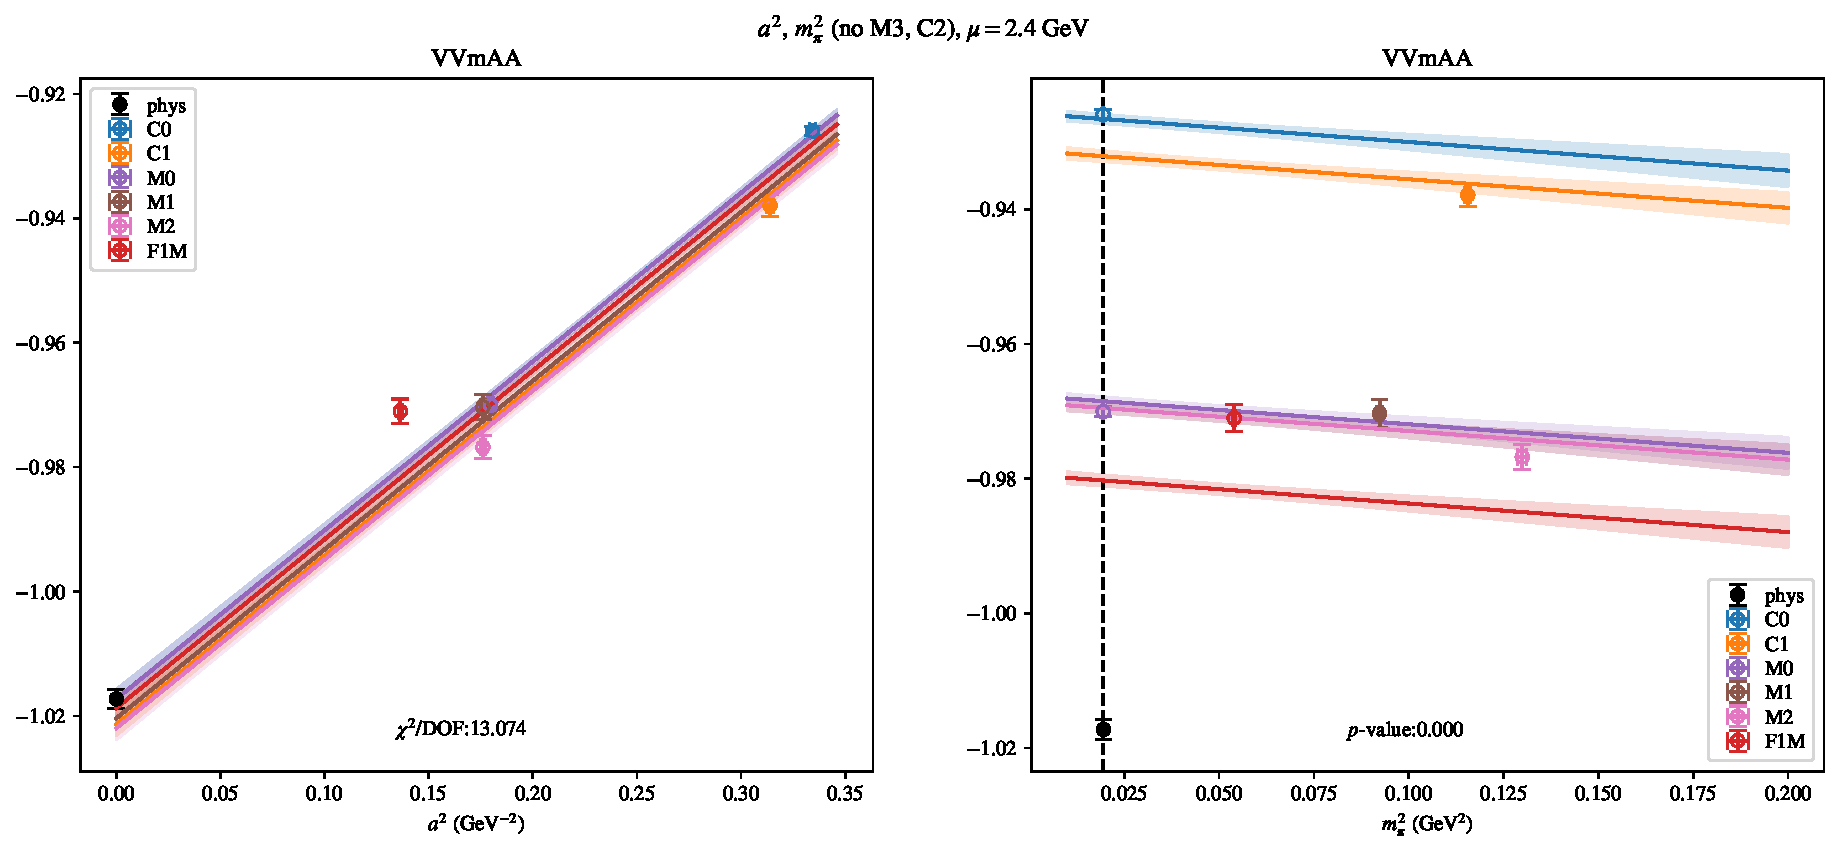
\includepdf[link, pages=-]{VVmAA/NPR/a2m2mcut_24.pdf}
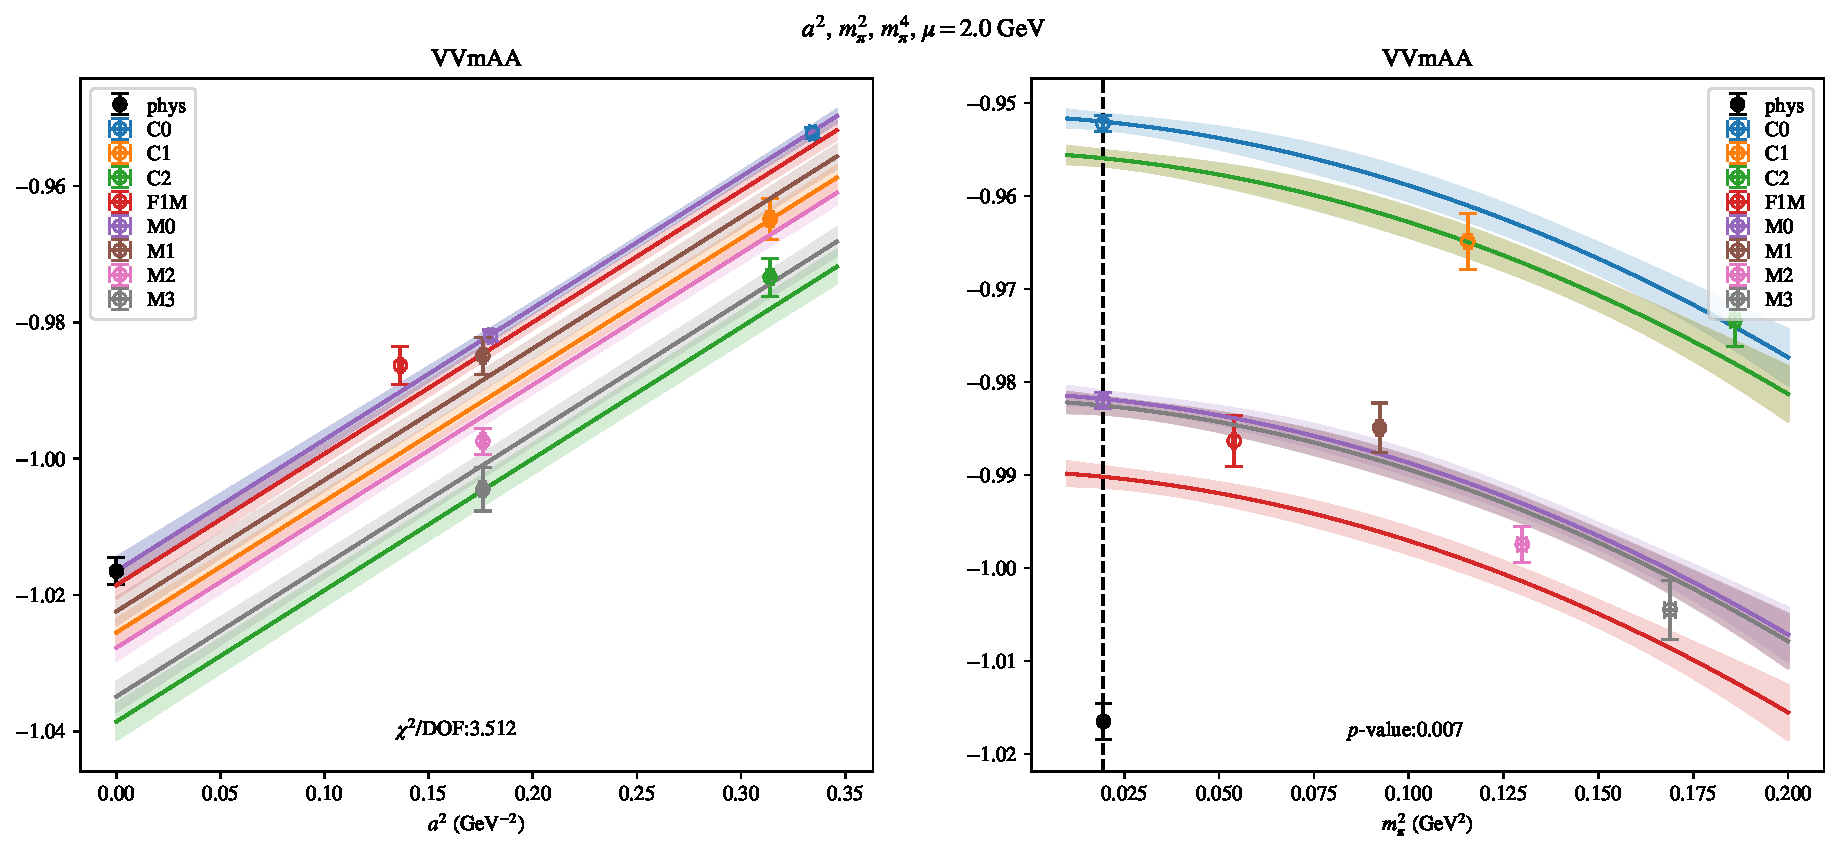
\includepdf[link, pages=-]{VVmAA/NPR/a2m2m4_20.pdf}
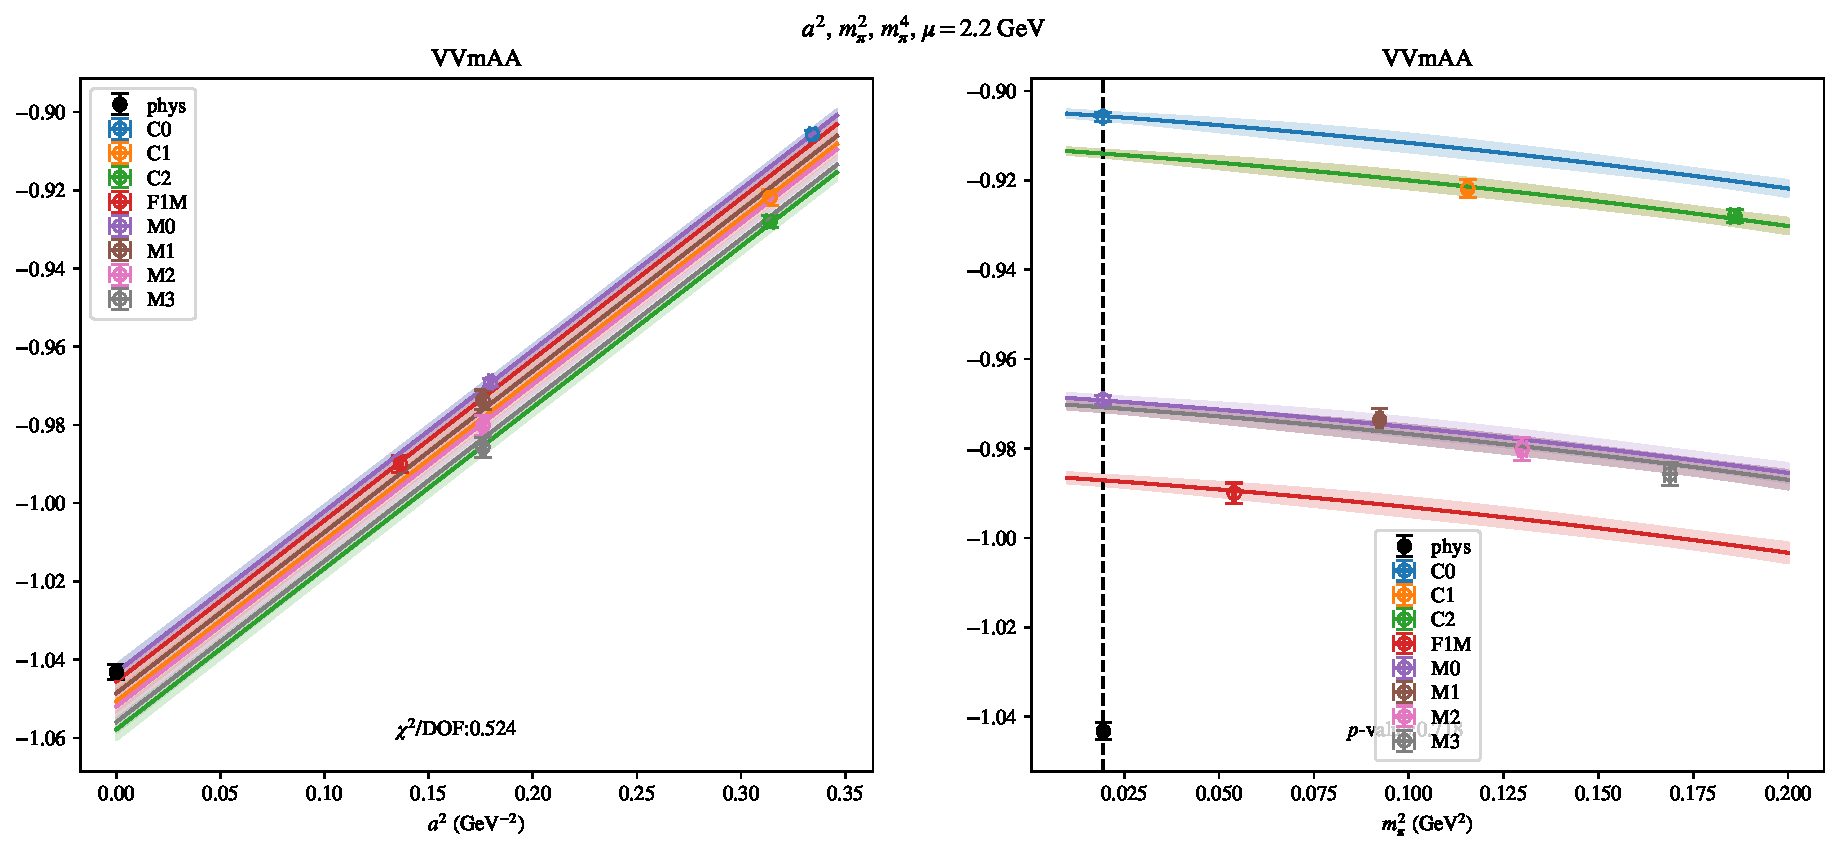
\includepdf[link, pages=-]{VVmAA/NPR/a2m2m4_22.pdf}
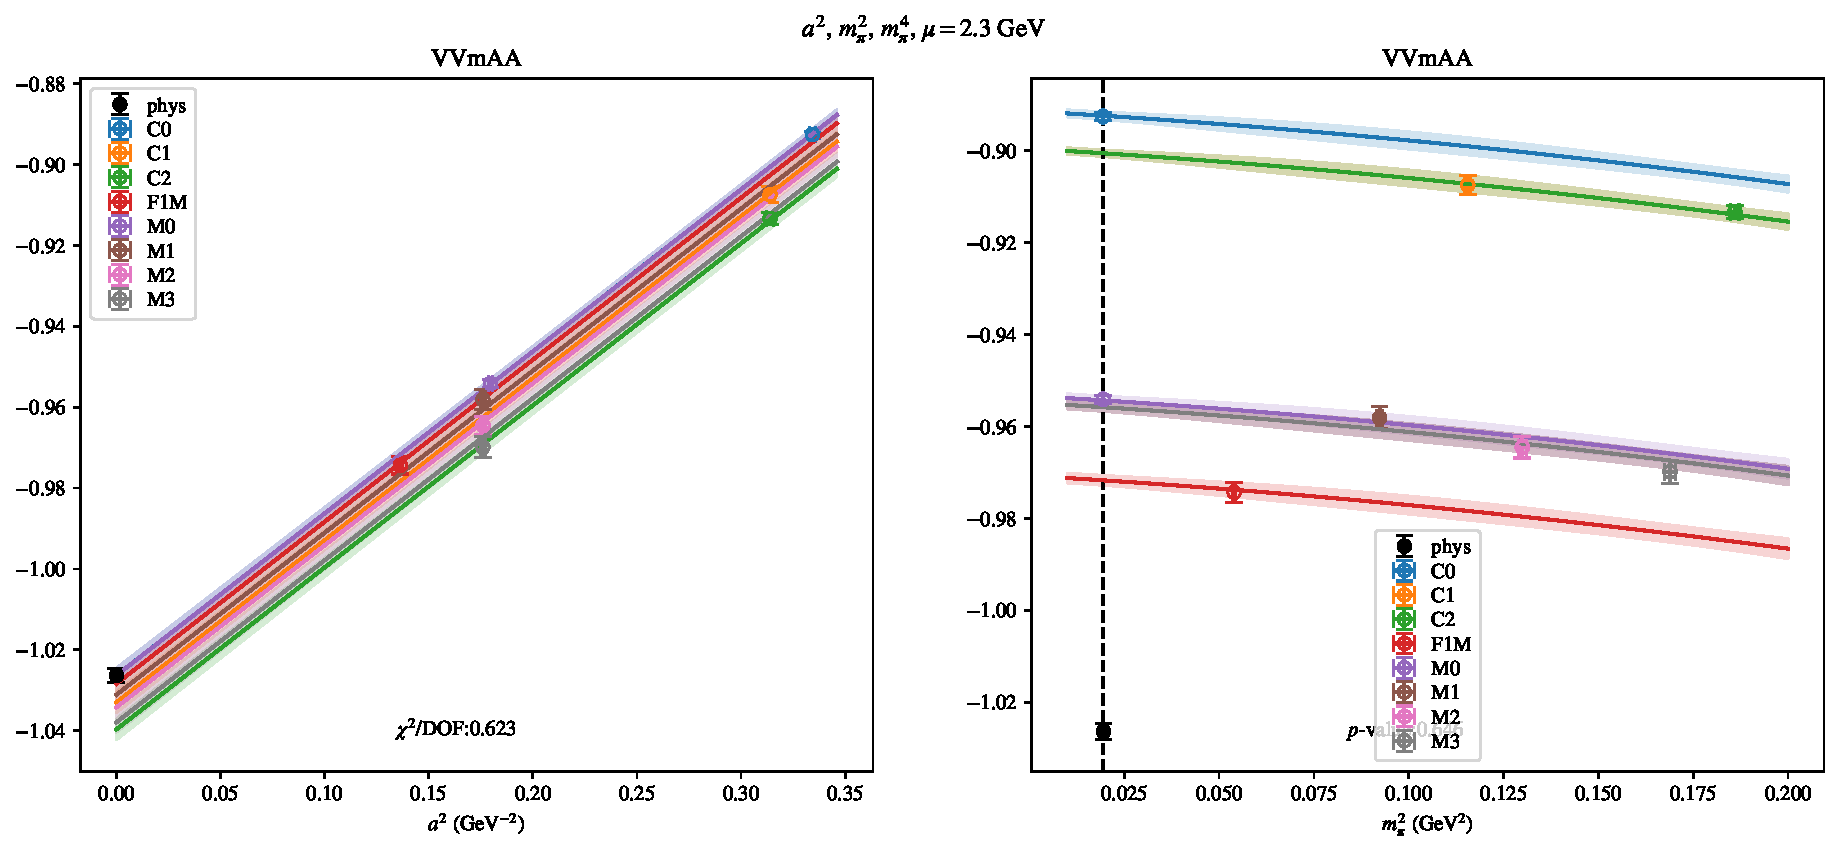
\includepdf[link, pages=-]{VVmAA/NPR/a2m2m4_23.pdf}
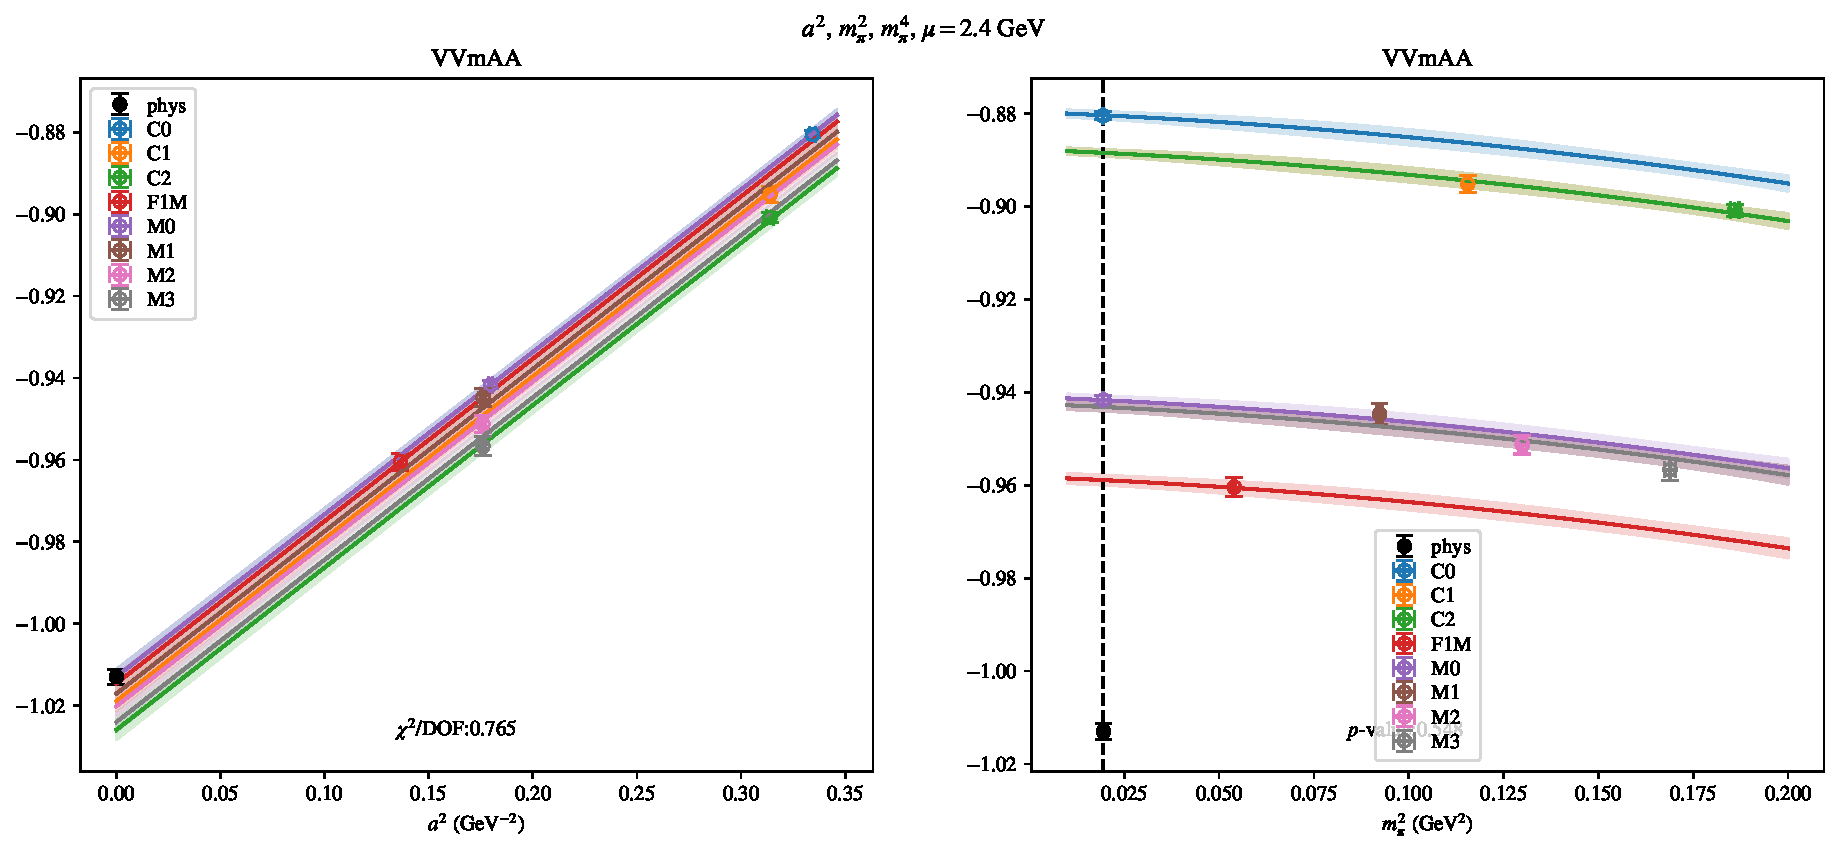
\includepdf[link, pages=-]{VVmAA/NPR/a2m2m4_24.pdf}
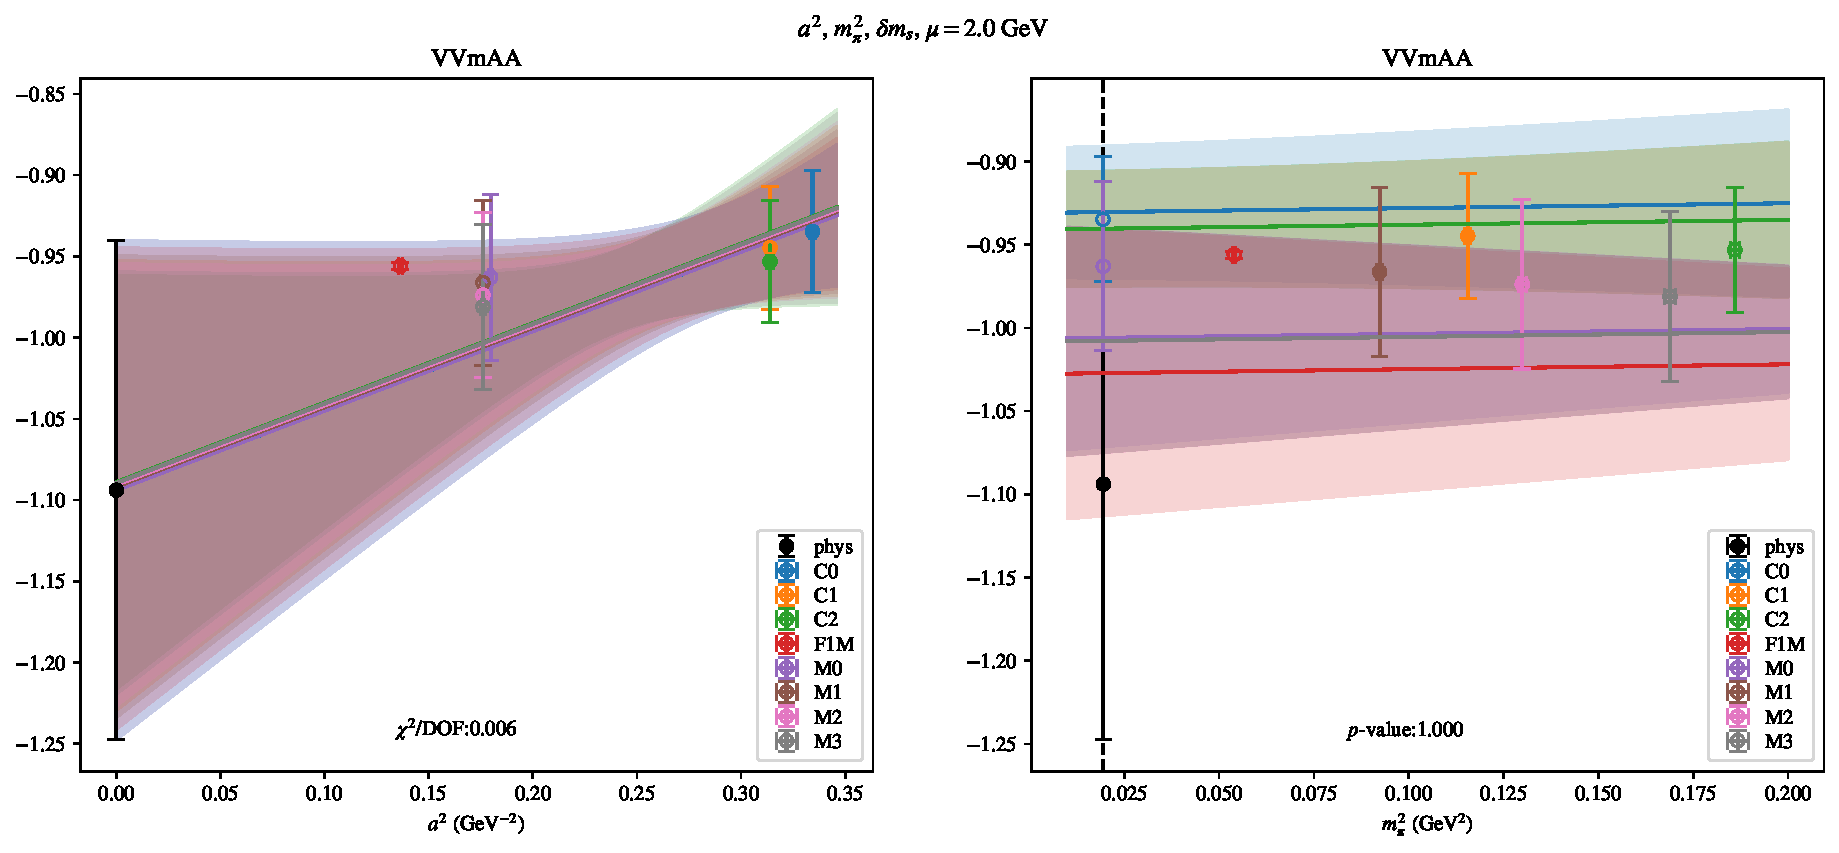
\includepdf[link, pages=-]{VVmAA/NPR/a2m2delm_20.pdf}
\includepdf[link, pages=-]{VVmAA/NPR/a2m2delm_22.pdf}
\includepdf[link, pages=-]{VVmAA/NPR/a2m2delm_23.pdf}
\includepdf[link, pages=-]{VVmAA/NPR/a2m2delm_24.pdf}
\clearpage
\section{$\mathcal{B}_3$}
\begin{table}[h!]
\begin{center}
\begin{tabular}{|c|c|c|c|c|c|c|}
\hline
$\mu$ (GeV) & $a^2$, $m_\pi^2$& $a^2$, $m_\pi^2$ (no C)& $a^2$, $m_\pi^2$, $a^4$& $a^2$, $m_\pi^2$ (no M3, C2)& $a^2$, $m_\pi^2$, $m_\pi^4$& $a^2$, $m_\pi^2$, $\delta m_s$\\
\hline
2.0& \hyperlink{SSmPP/NPR/a2m2_20.pdf.1}{\textbf{1.756(10)}: 5.142 (0.0)} & \hyperlink{SSmPP/NPR/a2m2noC_20.pdf.1}{\textbf{1.637(36)}: 0.375 (0.687)} & \hyperlink{SSmPP/NPR/a2a4m2_20.pdf.1}{\textbf{1.44(12)}: 0.506 (0.731)} & \hyperlink{SSmPP/NPR/a2m2mcut_20.pdf.1}{\textbf{1.7586(68)}: 6.802 (0.0)} & \hyperlink{SSmPP/NPR/a2m2m4_20.pdf.1}{\textbf{1.763(11)}: 6.397 (0.0)} & \hyperlink{SSmPP/NPR/a2m2delm_20.pdf.1}{\textbf{1.812(22)}: 0.355 (0.841)}\\
2.2& \hyperlink{SSmPP/NPR/a2m2_22.pdf.1}{\textbf{1.7874(59)}: 7.83 (0.0)} & \hyperlink{SSmPP/NPR/a2m2noC_22.pdf.1}{\textbf{1.703(20)}: 0.715 (0.489)} & \hyperlink{SSmPP/NPR/a2a4m2_22.pdf.1}{\textbf{1.576(55)}: 1.137 (0.337)} & \hyperlink{SSmPP/NPR/a2m2mcut_22.pdf.1}{\textbf{1.7862(64)}: 11.475 (0.0)} & \hyperlink{SSmPP/NPR/a2m2m4_22.pdf.1}{\textbf{1.7949(84)}: 8.325 (0.0)} & \hyperlink{SSmPP/NPR/a2m2delm_22.pdf.1}{\textbf{1.809(10)}: 1.017 (0.397)}\\
2.3& \hyperlink{SSmPP/NPR/a2m2_23.pdf.1}{\textbf{1.7875(62)}: 8.074 (0.0)} & \hyperlink{SSmPP/NPR/a2m2noC_23.pdf.1}{\textbf{1.712(21)}: 0.919 (0.399)} & \hyperlink{SSmPP/NPR/a2a4m2_23.pdf.1}{\textbf{1.580(53)}: 1.028 (0.391)} & \hyperlink{SSmPP/NPR/a2m2mcut_23.pdf.1}{\textbf{1.7905(82)}: 11.836 (0.0)} & \hyperlink{SSmPP/NPR/a2m2m4_23.pdf.1}{\textbf{1.7898(80)}: 8.056 (0.0)} & \hyperlink{SSmPP/NPR/a2m2delm_23.pdf.1}{\textbf{1.801(16)}: 1.146 (0.333)}\\
2.4& \hyperlink{SSmPP/NPR/a2m2_24.pdf.1}{\textbf{1.7928(57)}: 8.474 (0.0)} & \hyperlink{SSmPP/NPR/a2m2noC_24.pdf.1}{\textbf{1.713(18)}: 1.17 (0.31)} & \hyperlink{SSmPP/NPR/a2a4m2_24.pdf.1}{\textbf{1.600(43)}: 1.128 (0.341)} & \hyperlink{SSmPP/NPR/a2m2mcut_24.pdf.1}{\textbf{1.798(10)}: 12.748 (0.0)} & \hyperlink{SSmPP/NPR/a2m2m4_24.pdf.1}{\textbf{1.8019(70)}: 8.963 (0.0)} & \hyperlink{SSmPP/NPR/a2m2delm_24.pdf.1}{\textbf{1.8135(92)}: 1.097 (0.356)}\\
\hline
\end{tabular}
\caption{Physical point value from chiral and continuum extrapolation at renormalisation scale $\mu$. Entries are \textbf{value(error)}: $\chi^2/\text{DOF}$ ($p$-value).}
\end{center}
\end{table}
\begin{table}[h!]
\begin{center}
\begin{tabular}{|c c|c|c|c|c|c|c|}
\hline
$\mu$ (GeV) &  & $a^2$, $m_\pi^2$& $a^2$, $m_\pi^2$ (no C)& $a^2$, $m_\pi^2$, $a^4$& $a^2$, $m_\pi^2$ (no M3, C2)& $a^2$, $m_\pi^2$, $m_\pi^4$& $a^2$, $m_\pi^2$, $\delta m_s$\\
\hline
\multirow{3}{0.5in}{2.0} & $\alpha$ & 0.158(34)& 0.69(17)& 2.42(96)& 0.147(22)& 0.141(32)& 0.051(44)\\
 & $\beta$ & 0.00023(33)& -0.0006(42)& -0.0012(45)& -0.0& -0.0019(78)& -0.0008(23)\\
 & $\gamma$ &  &  & -4.(20)&  & 0.000170(96)& 0.0188(65)\\
\hline
\multirow{3}{0.5in}{2.2} & $\alpha$ & 0.093(18)& 0.425(87)& 1.43(39)& 0.099(19)& 0.088(18)& 0.059(19)\\
 & $\beta$ & -0.0001(13)& -0.0007(40)& -0.0009(22)& -0.0002(33)& -0.0020(96)& -0.0006(17)\\
 & $\gamma$ &  &  & -2.7(82)&  & 0.000179(88)& 0.0128(37)\\
\hline
\multirow{3}{0.5in}{2.3} & $\alpha$ & 0.108(16)& 0.399(86)& 1.42(37)& 0.113(18)& 0.121(25)& 0.095(36)\\
 & $\beta$ & -0.0001(16)& -0.0007(40)& -0.0009(22)& -0.0& -0.0025(75)& -0.0007(15)\\
 & $\gamma$ &  &  & -2.7(77)&  & 0.000221(68)& 0.0112(44)\\
\hline
\multirow{3}{0.5in}{2.4} & $\alpha$ & 0.109(15)& 0.405(74)& 1.29(29)& 0.092(31)& 0.086(20)& 0.072(20)\\
 & $\beta$ & -0.0001(14)& -0.0007(38)& -0.0008(20)& -0.0002(23)& -0.0027(70)& -0.0008(14)\\
 & $\gamma$ &  &  & -2.4(63)&  & 0.000227(65)& 0.0132(30)\\
\hline
\end{tabular}
\caption{Fit values of coefficients in $Q = Q_{phys} + \mathbf{\alpha} a^2 + \mathbf{\beta}\left(\frac{m_\pi^2}{f_\pi^2}-\frac{m_{\pi,PDG}^2}{f_\pi^2}\right) + \gamma(\ldots)$}
\end{center}
\end{table}
\includepdf[link, pages=-]{SSmPP/NPR/a2m2_20.pdf}
\includepdf[link, pages=-]{SSmPP/NPR/a2m2_22.pdf}
\includepdf[link, pages=-]{SSmPP/NPR/a2m2_23.pdf}
\includepdf[link, pages=-]{SSmPP/NPR/a2m2_24.pdf}
\includepdf[link, pages=-]{SSmPP/NPR/a2m2noC_20.pdf}
\includepdf[link, pages=-]{SSmPP/NPR/a2m2noC_22.pdf}
\includepdf[link, pages=-]{SSmPP/NPR/a2m2noC_23.pdf}
\includepdf[link, pages=-]{SSmPP/NPR/a2m2noC_24.pdf}
\includepdf[link, pages=-]{SSmPP/NPR/a2a4m2_20.pdf}
\includepdf[link, pages=-]{SSmPP/NPR/a2a4m2_22.pdf}
\includepdf[link, pages=-]{SSmPP/NPR/a2a4m2_23.pdf}
\includepdf[link, pages=-]{SSmPP/NPR/a2a4m2_24.pdf}
\includepdf[link, pages=-]{SSmPP/NPR/a2m2mcut_20.pdf}
\includepdf[link, pages=-]{SSmPP/NPR/a2m2mcut_22.pdf}
\includepdf[link, pages=-]{SSmPP/NPR/a2m2mcut_23.pdf}
\includepdf[link, pages=-]{SSmPP/NPR/a2m2mcut_24.pdf}
\includepdf[link, pages=-]{SSmPP/NPR/a2m2m4_20.pdf}
\includepdf[link, pages=-]{SSmPP/NPR/a2m2m4_22.pdf}
\includepdf[link, pages=-]{SSmPP/NPR/a2m2m4_23.pdf}
\includepdf[link, pages=-]{SSmPP/NPR/a2m2m4_24.pdf}
\includepdf[link, pages=-]{SSmPP/NPR/a2m2delm_20.pdf}
\includepdf[link, pages=-]{SSmPP/NPR/a2m2delm_22.pdf}
\includepdf[link, pages=-]{SSmPP/NPR/a2m2delm_23.pdf}
\includepdf[link, pages=-]{SSmPP/NPR/a2m2delm_24.pdf}
\clearpage
\section{$\mathcal{B}_4$}
\begin{table}[h!]
\begin{center}
\begin{tabular}{|c|c|c|c|c|c|c|}
\hline
$\mu$ (GeV) & $a^2$, $m_\pi^2$& $a^2$, $m_\pi^2$ (no C)& $a^2$, $m_\pi^2$, $a^4$& $a^2$, $m_\pi^2$ (no M3, C2)& $a^2$, $m_\pi^2$, $m_\pi^4$& $a^2$, $m_\pi^2$, $\delta m_s$\\
\hline
2.0& \hyperlink{SSpPP/NPR/a2m2_20.pdf.1}{\textbf{-0.925(56)}: 0.297 (0.915)} & \hyperlink{SSpPP/NPR/a2m2noC_20.pdf.1}{\textbf{-0.89(23)}: 0.3 (0.741)} & \hyperlink{SSpPP/NPR/a2a4m2_20.pdf.1}{\textbf{-0.83(68)}: 0.155 (0.961)} & \hyperlink{SSpPP/NPR/a2m2mcut_20.pdf.1}{\textbf{-0.916(81)}: 0.386 (0.763)} & \hyperlink{SSpPP/NPR/a2m2m4_20.pdf.1}{\textbf{-0.919(67)}: 0.302 (0.877)} & \hyperlink{SSpPP/NPR/a2m2delm_20.pdf.1}{\textbf{-0.93(16)}: 0.191 (0.943)}\\
2.2& \hyperlink{SSpPP/NPR/a2m2_22.pdf.1}{\textbf{-0.906(46)}: 0.61 (0.693)} & \hyperlink{SSpPP/NPR/a2m2noC_22.pdf.1}{\textbf{-0.91(13)}: 0.594 (0.552)} & \hyperlink{SSpPP/NPR/a2a4m2_22.pdf.1}{\textbf{-0.90(23)}: 0.815 (0.515)} & \hyperlink{SSpPP/NPR/a2m2mcut_22.pdf.1}{\textbf{-0.904(44)}: 0.685 (0.561)} & \hyperlink{SSpPP/NPR/a2m2m4_22.pdf.1}{\textbf{-0.906(53)}: 0.556 (0.695)} & \hyperlink{SSpPP/NPR/a2m2delm_22.pdf.1}{\textbf{-0.901(87)}: 0.808 (0.52)}\\
2.3& \hyperlink{SSpPP/NPR/a2m2_23.pdf.1}{\textbf{-0.897(49)}: 0.604 (0.697)} & \hyperlink{SSpPP/NPR/a2m2noC_23.pdf.1}{\textbf{-0.90(12)}: 0.781 (0.458)} & \hyperlink{SSpPP/NPR/a2a4m2_23.pdf.1}{\textbf{-0.87(33)}: 0.778 (0.539)} & \hyperlink{SSpPP/NPR/a2m2mcut_23.pdf.1}{\textbf{-0.895(44)}: 0.924 (0.428)} & \hyperlink{SSpPP/NPR/a2m2m4_23.pdf.1}{\textbf{-0.895(51)}: 0.629 (0.642)} & \hyperlink{SSpPP/NPR/a2m2delm_23.pdf.1}{\textbf{-0.899(75)}: 0.8 (0.525)}\\
2.4& \hyperlink{SSpPP/NPR/a2m2_24.pdf.1}{\textbf{-0.892(58)}: 0.708 (0.617)} & \hyperlink{SSpPP/NPR/a2m2noC_24.pdf.1}{\textbf{-0.89(11)}: 0.989 (0.372)} & \hyperlink{SSpPP/NPR/a2a4m2_24.pdf.1}{\textbf{-0.93(44)}: 0.948 (0.435)} & \hyperlink{SSpPP/NPR/a2m2mcut_24.pdf.1}{\textbf{-0.88(10)}: 1.014 (0.385)} & \hyperlink{SSpPP/NPR/a2m2m4_24.pdf.1}{\textbf{-0.886(54)}: 0.692 (0.598)} & \hyperlink{SSpPP/NPR/a2m2delm_24.pdf.1}{\textbf{-0.90(16)}: 0.833 (0.504)}\\
\hline
\end{tabular}
\caption{Physical point value from chiral and continuum extrapolation at renormalisation scale $\mu$. Entries are \textbf{value(error)}: $\chi^2/\text{DOF}$ ($p$-value).}
\end{center}
\end{table}
\begin{table}[h!]
\begin{center}
\begin{tabular}{|c c|c|c|c|c|c|c|}
\hline
$\mu$ (GeV) &  & $a^2$, $m_\pi^2$& $a^2$, $m_\pi^2$ (no C)& $a^2$, $m_\pi^2$, $a^4$& $a^2$, $m_\pi^2$ (no M3, C2)& $a^2$, $m_\pi^2$, $m_\pi^4$& $a^2$, $m_\pi^2$, $\delta m_s$\\
\hline
\multirow{3}{0.5in}{2.0} & $\alpha$ & 0.383(37)& 0.65(19)& 1.49(86)& 0.459(64)& 0.422(38)& 0.328(77)\\
 & $\beta$ & 0.00682(37)& 0.00737(65)& 0.00713(26)& 0.00805(80)& 0.00806(97)& 0.00643(45)\\
 & $\gamma$ &  &  & -2.(17)&  & -9.92353(86)& 0.0077(89)\\
\hline
\multirow{3}{0.5in}{2.2} & $\alpha$ & 0.432(24)& 0.39(10)& 0.46(27)& 0.453(30)& 0.423(28)& 0.444(34)\\
 & $\beta$ & 0.00693(16)& 0.00697(38)& 0.00699(19)& 0.00724(32)& 0.0076(10)& 0.00707(26)\\
 & $\gamma$ &  &  & -0.033&  & -6.88064(89)& -0.004(65)\\
\hline
\multirow{3}{0.5in}{2.3} & $\alpha$ & 0.455(30)& 0.38(10)& 0.69(39)& 0.462(25)& 0.459(30)& 0.444(40)\\
 & $\beta$ & 0.00698(20)& 0.00694(34)& 0.00714(26)& 0.00689(38)& 0.0076(10)& 0.00700(24)\\
 & $\gamma$ &  &  & -0.4(81)&  & -6.56312(90)& -0.0\\
\hline
\multirow{3}{0.5in}{2.4} & $\alpha$ & 0.452(41)& 0.408(90)& 0.004& 0.530(59)& 0.497(31)& 0.427(75)\\
 & $\beta$ & 0.00696(19)& 0.00697(33)& 0.00682(23)& 0.00691(37)& 0.0076(10)& 0.00682(36)\\
 & $\gamma$ &  &  & 0.945&  & -5.47982(96)& 0.0062(97)\\
\hline
\end{tabular}
\caption{Fit values of coefficients in $Q = Q_{phys} + \mathbf{\alpha} a^2 + \mathbf{\beta}\left(\frac{m_\pi^2}{f_\pi^2}-\frac{m_{\pi,PDG}^2}{f_\pi^2}\right) + \gamma(\ldots)$}
\end{center}
\end{table}
\includepdf[link, pages=-]{SSpPP/NPR/a2m2_20.pdf}
\includepdf[link, pages=-]{SSpPP/NPR/a2m2_22.pdf}
\includepdf[link, pages=-]{SSpPP/NPR/a2m2_23.pdf}
\includepdf[link, pages=-]{SSpPP/NPR/a2m2_24.pdf}
\includepdf[link, pages=-]{SSpPP/NPR/a2m2noC_20.pdf}
\includepdf[link, pages=-]{SSpPP/NPR/a2m2noC_22.pdf}
\includepdf[link, pages=-]{SSpPP/NPR/a2m2noC_23.pdf}
\includepdf[link, pages=-]{SSpPP/NPR/a2m2noC_24.pdf}
\includepdf[link, pages=-]{SSpPP/NPR/a2a4m2_20.pdf}
\includepdf[link, pages=-]{SSpPP/NPR/a2a4m2_22.pdf}
\includepdf[link, pages=-]{SSpPP/NPR/a2a4m2_23.pdf}
\includepdf[link, pages=-]{SSpPP/NPR/a2a4m2_24.pdf}
\includepdf[link, pages=-]{SSpPP/NPR/a2m2mcut_20.pdf}
\includepdf[link, pages=-]{SSpPP/NPR/a2m2mcut_22.pdf}
\includepdf[link, pages=-]{SSpPP/NPR/a2m2mcut_23.pdf}
\includepdf[link, pages=-]{SSpPP/NPR/a2m2mcut_24.pdf}
\includepdf[link, pages=-]{SSpPP/NPR/a2m2m4_20.pdf}
\includepdf[link, pages=-]{SSpPP/NPR/a2m2m4_22.pdf}
\includepdf[link, pages=-]{SSpPP/NPR/a2m2m4_23.pdf}
\includepdf[link, pages=-]{SSpPP/NPR/a2m2m4_24.pdf}
\includepdf[link, pages=-]{SSpPP/NPR/a2m2delm_20.pdf}
\includepdf[link, pages=-]{SSpPP/NPR/a2m2delm_22.pdf}
\includepdf[link, pages=-]{SSpPP/NPR/a2m2delm_23.pdf}
\includepdf[link, pages=-]{SSpPP/NPR/a2m2delm_24.pdf}
\clearpage
\section{$\mathcal{B}_5$}
\begin{table}[h!]
\begin{center}
\begin{tabular}{|c|c|c|c|c|c|c|}
\hline
$\mu$ (GeV) & $a^2$, $m_\pi^2$& $a^2$, $m_\pi^2$ (no C)& $a^2$, $m_\pi^2$, $a^4$& $a^2$, $m_\pi^2$ (no M3, C2)& $a^2$, $m_\pi^2$, $m_\pi^4$& $a^2$, $m_\pi^2$, $\delta m_s$\\
\hline
2.0& \hyperlink{TT/NPR/a2m2_20.pdf.1}{\textbf{-0.36(18)}: 0.001 (1.0)} & \hyperlink{TT/NPR/a2m2noC_20.pdf.1}{\textbf{-0.359(80)}: 0.165 (0.848)} & \hyperlink{TT/NPR/a2a4m2_20.pdf.1}{\textbf{-0.032}: 0.001 (1.0)} & \hyperlink{TT/NPR/a2m2mcut_20.pdf.1}{\textbf{-0.35(18)}: 0.001 (1.0)} & \hyperlink{TT/NPR/a2m2m4_20.pdf.1}{\textbf{-0.35(21)}: 0.001 (1.0)} & \hyperlink{TT/NPR/a2m2delm_20.pdf.1}{\textbf{-0.39(68)}: 0.001 (1.0)}\\
2.2& \hyperlink{TT/NPR/a2m2_22.pdf.1}{\textbf{-0.37(24)}: 0.007 (1.0)} & \hyperlink{TT/NPR/a2m2noC_22.pdf.1}{\textbf{-0.366(65)}: 0.256 (0.774)} & \hyperlink{TT/NPR/a2a4m2_22.pdf.1}{\textbf{-0.086}: 0.001 (1.0)} & \hyperlink{TT/NPR/a2m2mcut_22.pdf.1}{\textbf{-0.36(13)}: 0.01 (0.999)} & \hyperlink{TT/NPR/a2m2m4_22.pdf.1}{\textbf{-0.35(14)}: 0.007 (1.0)} & \hyperlink{TT/NPR/a2m2delm_22.pdf.1}{\textbf{-0.29(73)}: 0.002 (1.0)}\\
2.3& \hyperlink{TT/NPR/a2m2_23.pdf.1}{\textbf{-0.34(17)}: 0.007 (1.0)} & \hyperlink{TT/NPR/a2m2noC_23.pdf.1}{\textbf{-0.365(65)}: 0.325 (0.723)} & \hyperlink{TT/NPR/a2a4m2_23.pdf.1}{\textbf{-0.6(28)}: 0.001 (1.0)} & \hyperlink{TT/NPR/a2m2mcut_23.pdf.1}{\textbf{-0.37(19)}: 0.01 (0.999)} & \hyperlink{TT/NPR/a2m2m4_23.pdf.1}{\textbf{-0.37(22)}: 0.007 (1.0)} & \hyperlink{TT/NPR/a2m2delm_23.pdf.1}{\textbf{-0.33(44)}: 0.002 (1.0)}\\
2.4& \hyperlink{TT/NPR/a2m2_24.pdf.1}{\textbf{-0.38(28)}: 0.006 (1.0)} & \hyperlink{TT/NPR/a2m2noC_24.pdf.1}{\textbf{-0.362(59)}: 0.381 (0.683)} & \hyperlink{TT/NPR/a2a4m2_24.pdf.1}{\textbf{-0.1(20)}: 0.002 (1.0)} & \hyperlink{TT/NPR/a2m2mcut_24.pdf.1}{\textbf{-0.36(17)}: 0.009 (0.999)} & \hyperlink{TT/NPR/a2m2m4_24.pdf.1}{\textbf{-0.35(13)}: 0.008 (1.0)} & \hyperlink{TT/NPR/a2m2delm_24.pdf.1}{\textbf{-0.36(37)}: 0.003 (1.0)}\\
\hline
\end{tabular}
\caption{Physical point value from chiral and continuum extrapolation at renormalisation scale $\mu$. Entries are \textbf{value(error)}: $\chi^2/\text{DOF}$ ($p$-value).}
\end{center}
\end{table}
\begin{table}[h!]
\begin{center}
\begin{tabular}{|c c|c|c|c|c|c|c|}
\hline
$\mu$ (GeV) &  & $a^2$, $m_\pi^2$& $a^2$, $m_\pi^2$ (no C)& $a^2$, $m_\pi^2$, $a^4$& $a^2$, $m_\pi^2$ (no M3, C2)& $a^2$, $m_\pi^2$, $m_\pi^4$& $a^2$, $m_\pi^2$, $\delta m_s$\\
\hline
\multirow{3}{0.5in}{2.0} & $\alpha$ & -0.055& 0.019& 1(13)& 0.087& 0.20(40)& -0.5(85)\\
 & $\beta$ & 0.0040(58)& 0.00702(47)& 0.028(30)& 0.0104(78)& 0.0030(47)& 0.0043(46)\\
 & $\gamma$ &  &  & -(29)&  & 0.001& 0.021\\
\hline
\multirow{3}{0.5in}{2.2} & $\alpha$ & -0.4(46)& -0.2(11)& 32(57)& -0.059& 0.012& 0.68(84)\\
 & $\beta$ & 0.0042(43)& 0.00659(31)& 0.021(24)& 0.0043(48)& 0.0048(36)& 0.0106(49)\\
 & $\gamma$ &  &  & -71.817&  & 0.00029(67)& -0.1(11)\\
\hline
\multirow{3}{0.5in}{2.3} & $\alpha$ & 0.14(33)& -0.2(12)& -4.751& -0.3(40)& -0.3(42)& 0.058\\
 & $\beta$ & 0.0073(37)& 0.00653(28)& 0.0046(73)& 0.0086(50)& 0.0046(39)& 0.0079(27)\\
 & $\gamma$ &  &  & 10(38)&  & 0.00011(60)& -0.05(76)\\
\hline
\multirow{3}{0.5in}{2.4} & $\alpha$ & -0.5(57)& -0.2(10)& 9.3(99)& -0.2(34)& -0.1(27)& -0.1(49)\\
 & $\beta$ & 0.0076(39)& 0.00653(28)& 0.0112(51)& 0.0074(43)& 0.0050(37)& 0.0060(21)\\
 & $\gamma$ &  &  & -2(22)&  & 0.00014(60)& 0.006\\
\hline
\end{tabular}
\caption{Fit values of coefficients in $Q = Q_{phys} + \mathbf{\alpha} a^2 + \mathbf{\beta}\left(\frac{m_\pi^2}{f_\pi^2}-\frac{m_{\pi,PDG}^2}{f_\pi^2}\right) + \gamma(\ldots)$}
\end{center}
\end{table}
\includepdf[link, pages=-]{TT/NPR/a2m2_20.pdf}
\includepdf[link, pages=-]{TT/NPR/a2m2_22.pdf}
\includepdf[link, pages=-]{TT/NPR/a2m2_23.pdf}
\includepdf[link, pages=-]{TT/NPR/a2m2_24.pdf}
\includepdf[link, pages=-]{TT/NPR/a2m2noC_20.pdf}
\includepdf[link, pages=-]{TT/NPR/a2m2noC_22.pdf}
\includepdf[link, pages=-]{TT/NPR/a2m2noC_23.pdf}
\includepdf[link, pages=-]{TT/NPR/a2m2noC_24.pdf}
\includepdf[link, pages=-]{TT/NPR/a2a4m2_20.pdf}
\includepdf[link, pages=-]{TT/NPR/a2a4m2_22.pdf}
\includepdf[link, pages=-]{TT/NPR/a2a4m2_23.pdf}
\includepdf[link, pages=-]{TT/NPR/a2a4m2_24.pdf}
\includepdf[link, pages=-]{TT/NPR/a2m2mcut_20.pdf}
\includepdf[link, pages=-]{TT/NPR/a2m2mcut_22.pdf}
\includepdf[link, pages=-]{TT/NPR/a2m2mcut_23.pdf}
\includepdf[link, pages=-]{TT/NPR/a2m2mcut_24.pdf}
\includepdf[link, pages=-]{TT/NPR/a2m2m4_20.pdf}
\includepdf[link, pages=-]{TT/NPR/a2m2m4_22.pdf}
\includepdf[link, pages=-]{TT/NPR/a2m2m4_23.pdf}
\includepdf[link, pages=-]{TT/NPR/a2m2m4_24.pdf}
\includepdf[link, pages=-]{TT/NPR/a2m2delm_20.pdf}
\includepdf[link, pages=-]{TT/NPR/a2m2delm_22.pdf}
\includepdf[link, pages=-]{TT/NPR/a2m2delm_23.pdf}
\includepdf[link, pages=-]{TT/NPR/a2m2delm_24.pdf}
\clearpage
\end{document}